
\chapter{HyCube Java library}
\label{sec:library}

This chapter describes the \emph{HyCube} library - Java implementation. The library (a jar file) consists of core classes and interfaces (generic - allowing creating different implementations of a DHT), and \emph{HyCube}-specific classes, implementing the algorithms used by a \emph{HyCube} node. The jar file contains the compatibility information (Java version) and a default configuration file (\emph{hycube-default.cfg}). Individual configuration properties may be overwritten in the application-specific configuration files. The chapter presents the API, the architecture of the library and describes configuration of individual modules. The following sections are supposed to provide an overview and explain the main concepts being used. Details of individual classes/interfaces are provided in the \emph{Javadoc} documentation attached to the library.




\section{The API}

The library API is provided by several node service classes:

\begin{itemize}
	\renewcommand{\labelitemi}{$\bullet$}
	
	\item \emph{HyCubeSingleQueueNodeService}, \emph{HyCubeSingleQueueNodeServiceNonWakeable}
	\item \emph{HyCubeMultiQueueNodeService}, \emph{HyCubeMultiQueueNodeServiceNonWakeable}
	\item \emph{HyCubeSchedulingMultiQueueNodeService}
	\item \emph{HyCubeSimpleNodeService}, \emph{HyCubeSimpleSchedulingNodeService}
	
	%\item \emph{HyCubeSingleQueueNodeService}
	%\item \emph{HyCubeSingleQueueNodeServiceNonWakeable}
	%\item \emph{HyCubeMultiQueueNodeService}
	%\item \emph{HyCubeMultiQueueNodeServiceNonWakeable}
	%\item \emph{HyCubeSchedulingMultiQueueNodeService}
	%\item \emph{HyCubeSimpleNodeService}
	%\item \emph{HyCubeSimpleSchedulingNodeService}
	
\end{itemize}

Node services should be considered as the main API entry point, unless certain customizations are required, in which case other publicly accessible classes may be used. All node services implement the \emph{HyCubeNodeService} interface (defining operations performed in the node context). Individual node services realize various approaches for event processing and managing threads. Because individual node services manage threads differently, they expect different configuration parameters - specified in the configuration file, as well as parameters passed to the node service initializer method call (\emph{initialize}), and they may define additional service-specific methods (in addition to the \emph{HyCubeNodeService} interface methods).

This section focuses on the \emph{HyCubeNodeService} interface and the \emph{HyCubeSimpleNodeService} node service implementation, which may be used for majority of applications. Other node services are described in detail in Section \ref{sec:libNodeServices}. \emph{HyCubeSimpleNodeService} is a node service automatically determining the number of threads needed for processing events, based on the parameters specified upon the node service instance creation (\emph{initialize} method) - described in Table \ref{tab:libHyCubeSimpleNodeServiceInitializeParams}.


\begin{table}[H]
\begin{center}
\scriptsize
\begin{tabular}{p{6.0cm} p{9.0cm}}
	\hline
	\textbf{Method}																& \textbf{Description}					\\[1mm]
    \hline
	\textbf{\emph{Environment} environment}										& The environment object represents the external environment, defines the time provider and contains node configuration read from the configuration file (details in Sections \ref{sec:libEnvironment}, \ref{sec:libTimeProvider} and \ref{sec:libConfiguration}). In the simplest case, the \emph{DirectEnvironment} class instance (providing the system time time provider and scheduler) and the default parameter file may be used (used by default when the configuration file is not specified in the \emph{DirectEnvironment.initialize} method).			\\[1.5mm]
	\textbf{\emph{String} nodeIdString} / \textbf{\emph{NodeId} nodeId}}		& The node ID - a \emph{String} representation or a \emph{NodeID} object (\emph{HyCubeNodeId} instance is expected with the default configuration).		\\[1.5mm]
	\textbf{\emph{String} bootstrapNodeAddress}									& The bootstrap node network address. With the default configuration, the UDP/IP protocol is used, and the address format is: \emph{IP\_ADDRESS:PORT}. If the \emph{null} value is provided, the node does not perform the JOIN procedure and forms a DHT containing only itself (other nodes may connect to it).			\\[1.5mm]
	\textbf{\emph{JoinCallback} joinCallback}									& The callback object that is notified (by calling the \emph{joinReturned} method) when the JOIN operation terminates (the node joined the DHT). In most cases, the use of an instance of \emph{JoinWaitCallback} (providing blocking waiting for the JOIN to finish) is sufficient.			\\[1.5mm]
	\textbf{\emph{Object} callbackArg}											& An argument that will be passed to the \emph{JoinCallback.joinReturned} method.			\\[1.5mm]
	\textbf{\emph{int} blockingExtEventsNum}									& The number of custom blocking events processed by nodes (details in Section \ref{sec:libNodeServices}). For the default configuration, value 0 should specified (this the default value used in case the value is not specified).			\\[1.5mm]
	\textbf{\emph{boolean} wakeup}												& A flag determining whether blocking events should be interrupted when non-blocking operations are enqueued to be processed. The mechanism is described in detail in Section \ref{sec:libWakeables}. The value \emph{true} may be specified by default, in which case the node may be served by a single thread. Otherwise, at least two threads should be defined, as one of the threads would be blocked for most of the time by blocking waiting for incoming messages.			\\[1.5mm]
	\textbf{\emph{EventProcessingErrorCallback} errorCallback}					& Specifies the error callback object that will be notified (\emph{errorOccurred} method called) when a critical internal error occurs in a thread different than the API caller thread. When such an error is raised, the further processing should be terminated and the node instance should be discarded.			\\[1.5mm]
	\textbf{\emph{Object} errorCallbackArg}										& An object passed to the \emph{EventProcessingErrorCallback.errorOccurred} method when an error is raised.			\\[1.5mm]
    \hline
\end{tabular}
\end{center}
\caption{\emph{HyCubeSimpleNodeService.initialize} method parameters}
\label{tab:libHyCubeSimpleNodeServiceInitializeParams}
\end{table}




A node service represents a DHT node (connected to the DHT system), and the operations defined by \emph{HyCubeNodeService} interface may be performed in the node context (Table \ref{tab:libDescHyCubeNodeService}).



%\begin{table}
\begin{center}
\scriptsize
\begin{longtable}{p{6.5cm} p{8.5cm}}
	\hline
	\textbf{Method}																& \textbf{Description}					\\[1mm]
    \hline
	\textbf{\emph{Node} getNode}												& Returns the \emph{Node} class instance, representing the node			\\[1.5mm]
	\textbf{\emph{NetworkNodePointer} createNetworkNodePointer}					& Creates a network node pointer object from its string representation		\\[1.5mm]
    \textbf{\emph{void} setPublicAddress}										& Sets the node's public network address (in case the network address translation is used) - this address will be exposed to other nodes in messages			\\[1.5mm]
	\textbf{\emph{MessageSendInfo} send}										& Sends a message to the specified recipient from the local source port to the recipient's destination port. The method expects the following arguments: the message recipient ID (\emph{NodeId}), optional direct recipient (\emph{String} or \emph{NetworkNodePointer} representation of the network address), the message data (\emph{byte[]}), the ack callback object (\emph{AckCallback}) notified when the delivery confirmation is received, optional routing parameters (\emph{Object[]}) described in Section \ref{sec:libRoutingManager}, and a boolean flag indicating whether the call should be blocking or sending the message should be enqueued and performed in the background. The recipient ID, recipient network address, source port, destination port and message data may be aggregated in a \emph{DataMessage} class instance. 		\\[1.5mm]
	\textbf{\emph{LookupCallback} lookup}										& Initiates the node lookup procedure, for the specified node ID. The method arguments include the lookup node ID (\emph{NodeId}), the lookup callback object (\emph{LookupCallback}) notified when the lookup procedure terminates, passing the result of the operation to the \emph{lookupReturned} method, a callback argument (\emph{Object}) that will be passed to the \emph{lookupReturned} method call, and optional lookup parameters (\emph{Object[]}) described in Section \ref{sec:libLookupManager}.			\\[1.5mm]
	\textbf{\emph{SearchCallback} search}										& Initiates the search procedure, for the given number of closest nodes to the specified node ID. The method arguments include the search node ID (\emph{NodeId}), the search callback object (\emph{SearchCallback}) notified when the search procedure terminates, passing the result of the operation to the \emph{searchReturned} method, a callback argument (\emph{Object}) that will be passed to the \emph{searchReturned} method call, optional set of initial node pointers (\emph{NodePointer[]}) to which initial search requests should be sent, an optional flag indicating whether the exact match node should NOT be returned by any intermediate node (default value \emph{false}), and optional search parameters (\emph{Object[]}) described in Section \ref{sec:libSearchManager}.			\\[1.5mm]
	\textbf{\emph{PutCallback} put}												& Initiates the PUT operation, storing a resource in the DHT. The method arguments include the message recipient (\emph{NodePointer}) - the argument is optional (if not specified, the message will be routed), the resource key (\emph{BigInteger}), the resource object (\emph{HyCubeResource}), a callback object (\emph{PutCallback}) notified when the PUT operation is finished, passing the status of the operation to the \emph{putReturned} method call, and optional put parameters (\emph{Object[]}) described in Section \ref{sec:libDHTManager}.		\\[1.5mm]
	\textbf{\emph{RefreshPutCallback} refreshPut}								& Initiates the REFRESH\_PUT operation, refreshing the validity time of the resource in the DHT. The method arguments include the message recipient (\emph{NodePointer}) - the argument is optional (if not specified, the message will be routed), the resource key (\emph{BigInteger}), the resource descriptor (\emph{HyCubeResourceDescriptor}), a callback object (\emph{RefreshPutCallback}) notified when the REFRESH\_PUT operation is finished, passing the status of the operation to the \emph{refreshPutReturned} method call, and optional parameters (\emph{Object[]}) described in Section \ref{sec:libDHTManager}.			\\[1.5mm]
	\textbf{\emph{GetCallback} get}												& Initiates the GET operation, retrieving resources from the DHT. The method arguments include the message recipient (\emph{NodePointer}) - the argument is optional (if not specified, the message will be routed), the resource key (\emph{BigInteger}), the get criteria (\emph{HyCubeResourceDescriptor}), a callback object (\emph{GetCallback}) notified when the GET operation is finished, passing the results (resources) to the \emph{getReturned} method call, and optional get parameters (\emph{Object[]}) described in Section \ref{sec:libDHTManager}.			\\[1.5mm]
	\textbf{\emph{DeleteCallback} delete}										& Initiates the DELETE operation, deleting a resource from a node in the DHT. The method arguments include the message recipient (\emph{NodePointer}), the resource key (\emph{BigInteger}), the delete criteria (\emph{HyCubeResourceDescriptor}), a callback object (\emph{DeleteCallback}) notified when the DELETE operation is finished, passing the status of the operation to the \emph{deleteReturned} method call, and optional delete parameters (\emph{Object[]}) described in Section \ref{sec:libDHTManager}.			\\[1.5mm]
	\textbf{\emph{void} join}													& Performs the JOIN procedure, connecting to the specified bootstrap node, and notifying the specified join callback object when the procedure terminates			\\[1.5mm]
	\textbf{\emph{void} leave}													& Performs the LEAVE operation - should be called before the node is disconnected from the DHT and discarded.			\\[1.5mm]
	\textbf{\emph{LinkedBlockingQueue<ReceivedDataMessage>} registerPort}		& Registers an incoming messages port and returns a queue to which the received messages will be inserted.				\\[1.5mm]
	\textbf{\emph{void} registerMessageReceivedCallbackForPort}					& Registers a callback object for a port (the callbeck object will be notified when a message is received)				\\[1.5mm]
	\textbf{\emph{void} unregisterMessageReceivedCallbackForPort}				& Unregisters the message received callback for port			\\[1.5mm]
	\textbf{\emph{void} unregisterPort}											& Unregisters the port		\\[1.5mm]
	\textbf{\emph{void} registerMessageReceivedCallback}						& Registers a callback for incoming messages (when ports are not used - configuration). The callback object is notified when a message is received.			\\[1.5mm]
	\textbf{\emph{void} unregisterMessageReceivedCallback}						& Unregisters the message received callback (when ports are not used)			\\[1.5mm]
	\textbf{\emph{int} getMaxMessageLength}										& Returns the maximum allowed message length			\\[1.5mm]
	\textbf{\emph{int} getMaxMessageDataLength}									& Returns the maximum allowed message data length		\\[1.5mm]
	\textbf{\emph{boolean} isInitialized}										& Returns a boolean value indicating whether the service instance is initialized			\\[1.5mm]
	\textbf{\emph{boolean} isDiscarded}											& Returns a boolean value indicating whether the service instance is discarded			\\[1.5mm]
	\textbf{\emph{void} recover}												& Explicit execution of the recovery procedure			\\[1.5mm]
	\textbf{\emph{void} recoverNS}												& Explicit execution of the neighborhood set recovery procedure			\\[1.5mm]
	\textbf{\emph{void} discard}												& Discards the node service instance		\\[1.5mm]
    \hline
%\captionsetup{justification=centering}
\caption{Operations defined by \emph{HyCubeNodeService}}
\label{tab:libDescHyCubeNodeService}
\end{longtable}
\end{center}
%\end{table}







\section{Example of a node life cycle}

The listing below presents an exemplary application creating a node instance using the \emph{SimpleNodeService} service, registering an incoming messages port, sending a test message to itself, receiving the message, leaving the system and destroying the node instance.

\begin{lstlisting}[style=listing1noindentsmall]
public static void main(String[] args) {
  Environment environment = DirectEnvironment.initialize();
  JoinWaitCallback joinWaitCallback = new JoinWaitCallback();
  SimpleNodeService sns = HyCubeSimpleNodeService.initialize(environment, 
    HyCubeNodeId.generateRandomNodeId(4, 32), 
    "192.168.1.9:5000", "192.168.1.8:5000", joinWaitCallback, null, 0, true, null, null);
  LinkedBlockingQueue<ReceivedDataMessage> inMsgQueue = sns.registerPort((short)0);

  sendTestDataMessageToSelf(sns, "Test string");
  try {
    ReceivedDataMessage recMsg = inMsgQueue.take();
  } catch (InterruptedException e) {}
  System.out.println("Message received!: " + new String(recMsg.getData()));

  sns.discard();
  environment.discard();
}

public static void sendTestDataMessageToSelf(NodeService ns, String text) {
  MessageAckCallback mac = new WaitMessageAckCallback() {
    public void notifyDelivered(Object callbackArg) {
      super.notifyDelivered(callbackArg);
      System.out.println("Message DELIVERED.");
    }
    public void notifyUndelivered(Object callbackArg) {
      super.notifyUndelivered(callbackArg);
      System.out.println("Message UNDELIVERED");
    }
  };
  byte[] data = text.getBytes();
  DataMessage msg = new DataMessage(ns.getNode().getNodeId(), null, (short)0, (short)0, data);
  try {
    MessageSendInfo msi = ns.send(msg, mac, null);
    System.out.println("Message send info - serial no: " + msi.getSerialNo());
  } catch (NodeServiceException e) {}
}	
\end{lstlisting}










\section{Library architecture, core library classes and their implementations}
\label{sec:libClasses}

The core of the \emph{HyCube} library is a set of configurable classes allowing implementation of any DHT algorithm. The architecture is based on exchangeable components implementing certain interfaces, realizing individual system functions. \emph{HyCube} library provides implementation of these components, realizing the \emph{HyCube} algorithms.

Figure \ref{fig:HyCubeLibraryArchitecture} presents the core of the library, and individual classes/interfaces are described in Section \ref{sec:libClasses}. Section \ref{sec:libEventProcessing} describes the realized solutions for event processing. Section \ref{sec:libNodeServices} focuses on node services, which are wrapper classes for node instances, additionally providing event processing mechanisms.

\begin{figure}
\centering
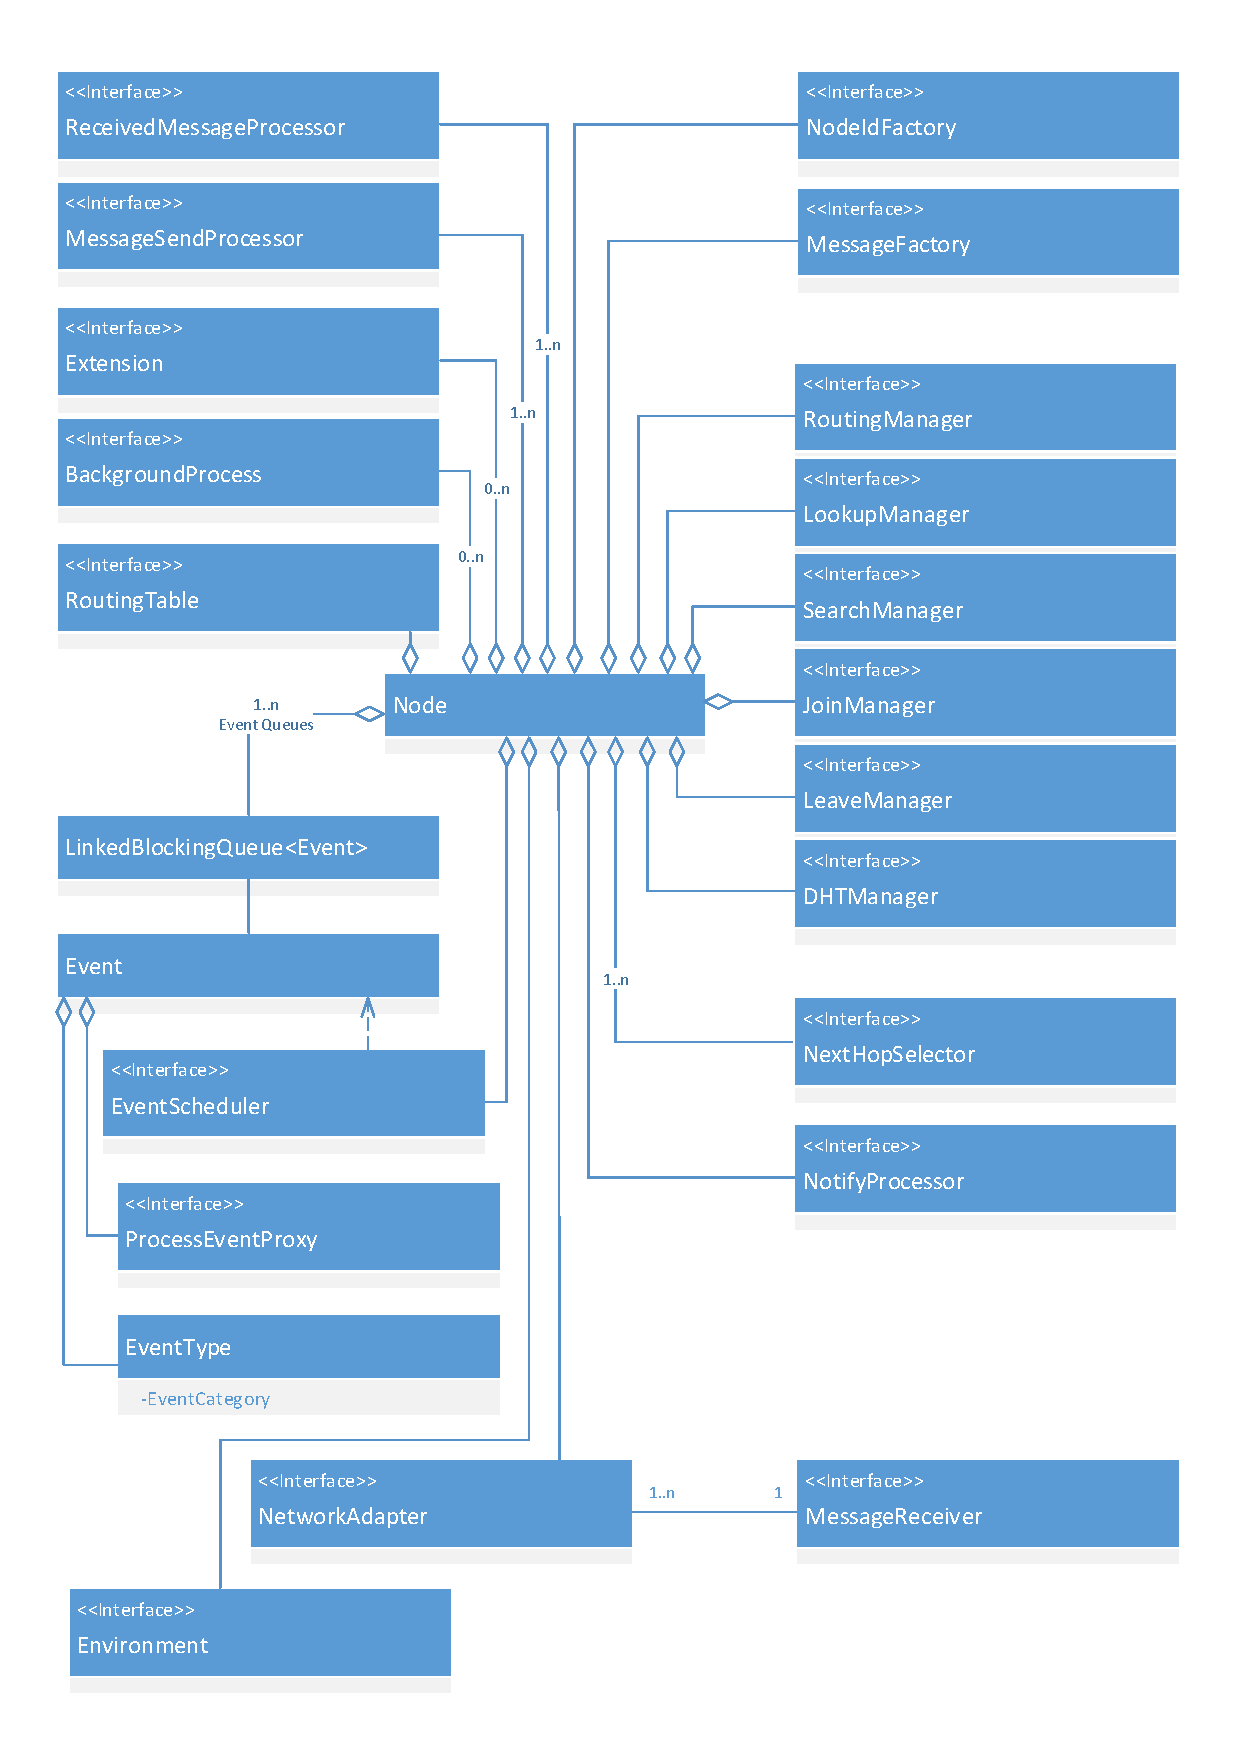
\includegraphics[trim = 10mm 10mm 10mm 10mm, clip, scale=.84]{img/HyCubeLibraryNode.pdf}
\caption{Node library architecture}
\label{fig:HyCubeLibraryArchitecture}
\end{figure}




\subsection{Node and library architecture}

The main class of the library is \emph{Node}. An instance of this class represents a DHT node and exposes the node interface to node services - operations such as \emph{join}, \emph{sendMessage}, \emph{lookup}, \emph{search}, \emph{put}, \emph{refreshPut}, \emph{get}, \emph{delete}, \emph{leave}, as well as methods registering incoming message queues (\emph{ReceivedDataMessage} instances) and callbacks (\emph{MessageReceivedCallback} instances). This class gathers the logic of all operations performed by nodes explicitly, as well as the processes taking place in the background. \emph{Node} is instantiated by calling one of the variants of its static method \emph{initializeNode}.

Most of the logic is realized by defining modules (classes) implementing certain interfaces, which are instantiated and initialized during the node initialization. Most of these modules (implementations) are defined in the configuration file (details in Section \ref{sec:libConfiguration}), but some of them are explicitly passed to the node initialization method upon creation (\emph{initialize}). Using the abstraction of individual modules, the node calls configured implementations as a result of the API, as well as internal calls.

Because individual components require full access to the node state, and often, to other dependent components, a special object, implementing \emph{NodeAccessor} interface, is passed to the components upon initialization \emph{initialize} method call (by the \emph{Node} instance). This object serves as a back-reference to the node instance, and may be used to access/modify node properties.




\subsection{Environment}
\label{sec:libEnvironment}

An object of a class extending abstract \emph{Environment} class is passed to the node initialization on creation. This object represents the external environment, defines the time provider and contains node configuration (read from the configuration file). The information passed to the \emph{Node} instance within the \emph{Environment} object may be extended and used by any module (accessed through the instance of \emph{NodeAccessor}). The default implementation of \emph{Environment} - \emph{DirectEnvironment} uses the system clock as the time provider, and reads configuration from a file (described in Section \ref{sec:libConfiguration}).




\subsection{Time provider}
\label{sec:libTimeProvider}

An object implementing \emph{TimeProvider} interface is passed to the \emph{Node} instance as a property of the \emph{Environment} object. The time provider object is expected to return a \emph{long} value, representing the current time. The interpretation of the time value returned is implementation specific. The default implementation \emph{SystemTimeProvider}, embedded in \emph{DirectEnvironment} class, uses the system clock (\emph{System.currentTimeMillis()} method) to retrieve the current time.

\emph{TimeProvider} provides also methods for scheduling tasks (instances of \emph{ScheduledTask}) for execution at a certain time in future. The default implementation uses the system clock (internally uses the \emph{ScheduledThreadPoolExecutor} class).




\subsection{Configuration}
\label{sec:libConfiguration}

Node configuration is passed to the \emph{Node} object on initialization, as a property of the \emph{Environment} object. The node properties are accessed though an object implementing the \emph{NodeProperties} interface. The methods of this interface allow access to the configuration properties for given property keys. The property keys and values are strings of characters. However, the \emph{NodeProperties} implementations should provide conversion of values to simple types defined in the \emph{ObjectToStringConverter.MappedType} enumeration, as well as conversion to enumerations (by default, the class \emph{ObjectToStringConverter} is used for the conversion). Additionally, \emph{NodeProperties} methods allow reading lists of values (of any type, including enumerations). Table \ref{tab:libConfTypes} presents the data types supported, as well as their formats.

\begin{table}
\scriptsize
\begin{center}
\begin{tabular}{p{3.5cm} p{4.0cm} p{7.0cm}}
	\hline
	\textbf{Corresponding Java type}	& \textbf{MappedType}					& \textbf{Format}					\\[1mm]
    \hline
	\textbf{Integer}			& \textbf{MappedType.INT}			& A signed decimal string representation, as expected by \emph{java.lang.Integer.Integer(String s)} constructor 				\\[1.5mm]
    \textbf{Short}				& \textbf{MappedType.SHORT}			& A signed decimal string representation, as expected by \emph{java.lang.Short.Short(String s)} constructor				\\[1.5mm]
	\textbf{Long}				& \textbf{MappedType.LONG}			& A signed decimal string representation, as expected by \emph{java.lang.Long.Long(String s)} constructor				\\[1.5mm]
	\textbf{Boolean}			& \textbf{MappedType.BOOLEAN}		& A string equal to \emph{true} or \emph{false}, as expected by \emph{java.lang.Boolean.Boolean(String s)} constructor	\\[1.5mm]
	\textbf{Float}				& \textbf{MappedType.FLOAT}			& A string representation of the \emph{float} value, as expected by \emph{java.lang.Float.Float(String s)} constructor			\\[1.5mm]
	\textbf{Double}				& \textbf{MappedType.DOUBLE}		& A string representation of the \emph{double} value, as expected by \emph{java.lang.Double.Double(String s)} constructor			\\[1.5mm]
	\textbf{Decimal}			& \textbf{MappedType.DECIMAL}		& A string representation of a decimal number, as expected by the constructor \emph{java.math.BigDecimal.BigDecimal(String val)}		\\[1.5mm]
	\textbf{BigInteger}			& \textbf{MappedType.BIGINTEGER}	& A decimal string representation of a big integer, as expected by the constructor \emph{ java.math.BigInteger.BigInteger(String val)}	\\[1.5mm]
	\textbf{Date}				& \textbf{MappedType.DATE}			& yyyy-MM-dd HH:mm:ss.SSS						\\[1.5mm]
	\textbf{String}				& \textbf{MappedType.STRING}		& -												\\[1.5mm]
	\textbf{Enum}				& \textbf{Separate conversion methods are defined for enumerations}					& Enumerations are converted using \emph{Enum.valueOf(Class<T>, String)} and \emph{Enum.toString()} methods.							\\[1.5mm]
	\textbf{List}				& \textbf{MappedType.LIST}			& A list of elements of any of the types described above. The list elements are, by default, separated by the comma (``,'') character			\\[1.5mm]
    \hline
\end{tabular}
\end{center}
\caption{Configuration - property types}
\label{tab:libConfTypes}
\end{table}

The default configuration technique employed by \emph{HyCube} uses \emph{ReaderNodeProperties} class, which reads configuration using an abstract reader object. The properties are, in the standard implementation of the \emph{Environment} class (\emph{DirectEnvironment}), read from a file (standard Java properties file format), using the \emph{FileNodePropertiesReader} class (implementation of NodePropertiesReader). \emph{FileNodePropertiesReader} reads properties from two files - default properties file and the application properties file, overwriting any property value redefined in the application properties file. Both properties files are expected to be located in the classpath of the application, and, if the default properties file name is not specified, the file name ``\emph{hycube\_default.cfg}'' is used (the name of the default configuration file delivered with the library).


The configuration architecture allows defining hierarchy of properties by separating keys at individual levels by the ``.'' character. \emph{NodeProperties} contains methods returning lower-level nested \emph{NodeProperties} objects. Such an approach may be used for configuration of nested components, by passing the nested configuration (\emph{NodeProperties}) objects to nested components. For example, for the following properties:

\begin{lstlisting}[style=listing1noindent]
Node.PropertyKey1 = PropertyValue1
Node.PropertyKey2 = PropertyValue2
Node.Module1.PropertyKey3 = PropertyValue3
Node.Module1.PropertyKey4 = PropertyValue4
\end{lstlisting}

\noindent
it is possible to access ``Node.Module1.*'' properties by a nested instance of \emph{NodeProperties}, using property keys, relative to ``Node.Module1'', for example ``PropertyKey3''.

Moreover, \emph{HyCube} configuration allows definition of nested properties (keys) using a different notation:

\begin{lstlisting}[style=listing1noindent]
Node[Module1].PropertyKey3 = PropertyValue3
Node[Module1].PropertyKey4 = PropertyValue4
\end{lstlisting}

\noindent
The effect is the same as in the previous example. However, such a notation allows easier identification of properties for subcomponents, for example:

\begin{lstlisting}[style=listing1noindent]
Node.RoutingModuleKeys = Module1, Module2
Node.RoutingModules[Module1].PropertyKey1 = PropertyValue1
Node.RoutingModules[Module2].PropertyKey1 = PropertyValue1
\end{lstlisting}

\noindent
Such properties may be accessed by retrieving nested properties until the lowest-level is reached, by specifying the full property key, or by specifying the key ``Node.RoutingModules'' (possibly just ``RoutingModules'' on the nested \emph{NodeProperties} object) and specifying ``Module1'' or ``Module2'' as the ``element name''. All three methods are supported by the \emph{HyCube} configuration API.


\emph{ReaderNodeProperties} allows specifying the property determining the name space of the configuration (by default the property name is ``configuration''). Such an approach makes it very easy to switch between many configuration variants stored within the same file, for example:

\begin{lstlisting}[style=listing1noindent]
configuration = node.main
# configuration = node.simulation

node.main.Property1 = Value1
node.main. ...

node.simulation.Property1 = Value2
node.simulation. ...
\end{lstlisting}

\noindent
making is possible to switch the whole configuration by changing the value of only one property - \emph{configuration}. The \emph{Node} instance, within the \emph{Environment} object, receives the \emph{NodeProperties} instance, representing a nested element defined by the configuration name space and nested \emph{NodeProperties} instances are passed to individual components.

The character ``\#'' at the beginning of a line denotes a comment, and causes that such a line is not processed by the configuration reader. It is also possible to use pointers (@ symbol) in the configuration to point property values (or whole nested properties sets) defined under a different key, for example:

\begin{lstlisting}[style=listing1noindent]
Node.RoutingModuleKeys = Module1, Module2, Module3
Node.RoutingModules[Module1].PropertyKey1 = @conf1.PropertyValueX
Node.RoutingModules[Module2].PropertyKey1 = @conf1.PropertyValueX

Node.RoutingModules[Module3] = @Node.RoutingModules[Module1]

conf1.PropertyValueX = PropertyValue1
\end{lstlisting}

\noindent
Whenever the symbol ``@'' is found at the beginning of the property value, the value (or the whole nested properties set) is first retrieved from the property that the symbol ``@'' points. Such a feature may become very useful when semantically the same property is a configuration parameter of multiple modules. In such a case, it is possible to define that property once, and use pointers to set the same value in configuration of all modules. The pointers mechanism is recursive, so multiple pointers may be used before the final value is obtained. In the above example, the property ``PropertyValue1'' for a nested \emph{NodeProperties} object (representing ``Node.RoutingModules[Module3]'') would have value ``PropertyValue1''. Two pointers are resolved while retrieving the value. However, the pointer would be resolved only when the value or the nested property retrieved is the pointer itself. The pointer ``@Node.RoutingModules[Module1]'' would not be resolved in the example above, if the property ``Node.RoutingModules[Module3].PropertyValue1'' was requested on an \emph{NodeProperties} object relative to the root of the configuration.

For module (configurable objects created dynamically), a convention has been adopted to define a key (or keys) representing the module instances and configure their properties using the [] notation. Additionally, when the implementing class (of the module) is configurable, a property ``Class'' is introduced on the module level (defining the full class name). This property should be read by the parent module - the class name should be known to instantiate the child module. An example (configuration of the node ID factory and exemplary extensions) is presented in the listing below:

\begin{lstlisting}[style=listing1noindent, mathescape]
configuration = node

node.NodeIdFactory = HyCubeNodeIdFactory
node.NodeIdFactory[HyCubeNodeIdFactory].Class 
                 $\hookrightarrow$   = net.hycube.core.HyCubeNodeIdFactory
node.NodeIdFactory[HyCubeNodeIdFactory].Dimensions = 4
node.NodeIdFactory[HyCubeNodeIdFactory].Levels = 32

node.Extensions = KeepAliveExtension, RecoveryExtension, ...
node.Extensions[KeepAliveExtension].Class 
                 $\hookrightarrow$   = net.hycube.maintenance.HyCubeKeepAliveExtension
node.main.Extensions[KeepAliveExtension].PingInterval = 5000
...
node.Extensions[RecoveryExtension].Class
                 $\hookrightarrow$   = net.hycube.maintenance.HyCubeRecoveryExtension
...
\end{lstlisting}



\begin{table}
\scriptsize
\begin{center}
\begin{tabular}{p{3.5cm} p{2.5cm} p{8.5cm}}
	\hline
	\textbf{Property}					& \textbf{Type}				& \textbf{Value}					\\[1mm]
    \hline
    \textbf{MessageTTL}					& \textbf{Integer}				& The TTL - maximum route length													\\[1.5mm]
	\textbf{MessageAckEnabled}			& \textbf{Boolean}				& Determines whether the message delivery acknowledgments should be sent			\\[1.5mm]
	\textbf{DirectAck}					& \textbf{Boolean}				& Determines whether ACK message are sent directly to the sender or routed			\\[1.5mm]
	\textbf{AckTimeout}					& \textbf{Integer}				& The waiting time (milliseconds) for an ACK message, after which the original message is considered undelivered 			\\[1.5mm]
	\textbf{ProcessAckInterval}			& \textbf{Integer}				& The schedule interval for the background process processing awaiting ACK messages		\\[1.5mm]
	\textbf{ResendIfNoAck}				& \textbf{Boolean}				& Determines whether messages should be resent when no ACK is received					\\[1.5mm]
	\textbf{SendRetries}				& \textbf{Integer}				& Determines how many times messages should be resent if they are not delivered			\\[1.5mm]
	\textbf{NodeIdFactory}				& \textbf{Nested (+ Class)}		& The configuration of the node ID factory module										\\[1.5mm]
	\textbf{MessageFactory}				& \textbf{Nested (+ Class)}		& The configuration of the message factory module										\\[1.5mm]
	\textbf{RoutingTable}				& \textbf{Nested (+ Class)}		& The configuration of the routing table structure module								\\[1.5mm]
	\textbf{NextHopSelectors}			& \textbf{Nested (+ Class)}		& The configuration of the next hop selectors. Multiple next hop selectors may be defined.		\\[1.5mm]
	\textbf{RoutingManager}				& \textbf{Nested (+ Class)}		& The configuration of the routing manager module										\\[1.5mm]
	\textbf{LookupManager}				& \textbf{Nested (+ Class)}		& The configuration of the lookup manager module										\\[1.5mm]
	\textbf{SearchManager}				& \textbf{Nested (+ Class)}		& The configuration of the search manager module										\\[1.5mm]
	\textbf{JoinManager}				& \textbf{Nested (+ Class)}		& The configuration of the join manager module											\\[1.5mm]
	\textbf{LeaveManager}				& \textbf{Nested (+ Class)}		& The configuration of the leave manager module											\\[1.5mm]
	\textbf{DHTManager}					& \textbf{Nested (+ Class)}		& The configuration of the DHT manager module											\\[1.5mm]
	\textbf{NotifyProcessor}			& \textbf{Nested (+ Class)}		& The configuration of the notify processor module										\\[1.5mm]
	\textbf{NetworkAdapter}				& \textbf{Nested (+ Class)}		& The configuration of the network adapter module										\\[1.5mm]
	\textbf{MessageReceiver}			& \textbf{Nested (+ Class)}		& The configuration of the message receiver module										\\[1.5mm]
	\textbf{ReceivedMessageProcessors}	& \textbf{Nested (+ Class)}		& The configuration of the received message processors (multiple entries)				\\[1.5mm]
	\textbf{MessageSendProcessors}		& \textbf{Nested (+ Class)}		& The configuration of the message send processors (multiple entries)					\\[1.5mm]
	\textbf{Extensions}					& \textbf{Nested (+ Class)}		& The configuration of the extension modules (multiple entries)							\\[1.5mm]
	\textbf{BackgroundProcesses}		& \textbf{Nested (+ Class)}		& The configuration of the background process modules (multiple entries)				\\[1.5mm]
    \hline
\end{tabular}
\end{center}
\caption{Node configuration properties}
\label{tab:libPropNode}
\end{table}


After instantiating a module instance, as a rule, the initialization (\emph{initialize()}) method of the created object is called, passing the configuration (a nested \emph{NodeProperties} object) and the node accessor to the module. Module's \emph{discard} method should be used to release all resources maintained by the module and perform any operations necessary when the module is disconnected from the node instance. This method is called by the \emph{Node} object when the module is discarded.

The properties at the node level (used by the \emph{Node} class) are described in Table \ref{tab:libPropNode}. The properties of individual component implementations are presented in the following sections. It is also possible to define environment-level parameters by specifying the nested configuration - ``Environment'' property at the root namespace level. Table \ref{tab:libDirectEnvironment} specifies the configuration of \emph{DirectEnvironment}.

\begin{table}
\scriptsize
\begin{center}
\begin{tabular}{p{5cm} p{2cm} p{7.5cm}}
	\hline
	\textbf{Property}									& \textbf{Type}									& \textbf{Value}																	\\[1mm]
    \hline
	\textbf{Environment}								& \textbf{String}								& \textit{DirectEnvironment}														\\[1.5mm]
    \textbf{Environment[DirectEnvironment] \newline $\hookrightarrow$.SchedulerThreadPoolSize}			& \textbf{Integer}							& The number of threads used by the system clock scheduler. This parameter is optional - if not specified, the default value (1) is used.							\\[1.5mm]
    \hline
\end{tabular}
\end{center}
\caption{DirectEnvironment configuration properties}
\label{tab:libDirectEnvironment}
\end{table}





\subsection{Node ID factory, Node ID}

Classes implementing \emph{NodeId} interface represent node identifiers. To allow dynamic creation of node ID instances, based on their binary or text representation, a factory class (implementing \emph{NodeIdFactory} interface) should be defined. The methods of the factory object would return the instances of the node IDs of a specific type. The implementations of classes \emph{NodeId} and \emph{NodeIdFactory} define the object-byte and byte-object conversion for the node IDs, as well as comparisons and other operations on the node IDs.

To represent the node ID in \emph{HyCube}, the class \emph{HyCubeNodeId} and the factory class \emph{HyCubeNodeIdFactory} (implementing the interfaces described) are used. \emph{HyCubeNodeIdFactory} class should be configured for a certain number of dimensions and hierarchy levels (of the hierarchical hypercube), and returns instances of \emph{HyCubeNodeId} class for the configured numbers of dimensions and hierarchy levels. The properties that should be configured for \emph{HyCubeNodeIdFactory} module are presented in Table \ref{tab:libPropHyCubeNodeIdFactory}.

\begin{table}
\scriptsize
\begin{center}
\begin{tabular}{p{3cm} p{3cm} p{8.5cm}}
	\hline
	\textbf{Property}			& \textbf{Type}				& \textbf{Value}					\\[1mm]
    \hline
	\textbf{Class}				& \textbf{String}			& \textit{net.hycube.core.HyCubeNodeIdFactory}				\\[1.5mm]
    \textbf{Dimensions}			& \textbf{Integer}			& The number of dimensions									\\[1.5mm]
	\textbf{Levels}				& \textbf{Integer}			& The number of hierarchy levels							\\[1.5mm]
    \hline
\end{tabular}
\end{center}
\caption{HyCubeNodeIdFactory configuration properties}
\label{tab:libPropHyCubeNodeIdFactory}
\end{table}



\subsection{Routing table}

Because the core of the library may be used for implementation of many different DHT systems, the structure of the routing table may vary depending on the overlay structure. The class representing the routing table should implement the \emph{RoutingTable} interface. \emph{HyCubeRoutingTableImpl} is a class implementing the \emph{RoutingTable} interface, reflecting the structure of routing tables supported by nodes in \emph{HyCube}: the primary routing table, the secondary routing table and the neighborhood set. Classes operating on the routing tables should cast the maintained routing table object to \emph{HyCubeRoutingTableImpl}, and would then be able to access the \emph{HyCube}-specific structure. \emph{HyCubeRoutingTableImpl} configurable properties are presented in Table \ref{tab:libPropHyCubeRoutingTableImpl} 

\begin{table}
\scriptsize
\begin{center}
\begin{tabular}{p{3cm} p{3cm} p{8.5cm}}
	\hline
	\textbf{Property}				& \textbf{Type}				& \textbf{Value}					\\[1mm]
    \hline
	\textbf{Class}					& \textbf{String}			& \textit{net.hycube.core.HyCubeRoutingTableImpl}			\\[1.5mm]
    \textbf{Dimensions}				& \textbf{Integer}			& The number of dimensions													\\[1.5mm]
	\textbf{Levels}					& \textbf{Integer}			& The number of hierarchy levels											\\[1.5mm]
	\textbf{NSSize}					& \textbf{Integer}			& The size of the neighborhood set											\\[1.5mm]
	\textbf{RoutingTableSlotSize}	& \textbf{Integer}			& The maximum number of nodes that may be stored in the routing table slot	\\[1.5mm]
	\textbf{UseSecureRouting}		& \textbf{Boolean}			& Determines whether the secure routing tables should be maintained			\\[1.5mm]
    \hline
\end{tabular}
\end{center}
\caption{HyCubeRoutingTableImpl configuration properties}
\label{tab:libPropHyCubeRoutingTableImpl}
\end{table}


The class \emph{RoutingTableEntry} is used to store routing table entry information (for individual references). A routing table entry contains the node pointer (\emph{NodePointer} class, which consists of the node ID and the node's network pointer - a network layer specific class implementing the \emph{NetworkNodePointer} interface). In addition to a node pointer, routing table entries store the entry creation time, the distance to the node, a reference to the routing table slot containing the entry (routing table implementation specific), information whether the entry is enabled (used in next hop selection), discarded (the node should be removed). Furthermore, the routing table entry contains a map of additional data (objects) managed by individual modules. The map may be used to store the LNS/PNS indicators, cached results of extensive calculations performed for nodes, and many other. The map keys used by individual modules should be unique to avoid conflicts.




\subsection{Message factory}

A configurable message factory class should be an implementation of \emph{MessageFactory} interface. The message factory object is responsible for creating message instances (instances of a class implementing \emph{Message} interface). The implementations of \emph{Message} and \emph{MessageFactory} are responsible for message creation, object-byte and byte-object conversion, as well as message header definition, and any other operations performed on the message objects.

The implementations specific to the \emph{HyCube} protocol are \emph{HyCubeMessage} and \emph{HyCubeMessageFactory}. The header contains all the fields defined in Appendix \ref{sec:protocol}. Furthermore, the \emph{HyCubeMessageFactory} may be configured to include additional header fields that may be used by modules (values are defined during object creation, or using getters/setters). The configuration parameters of \emph{HyCubeMessageFactory} are presented in Table \ref{tab:libPropHyCubeMessageFactory}.

\begin{table}
\scriptsize
\begin{center}
\begin{tabular}{p{3.5cm} p{2.5cm} p{8.5cm}}
	\hline
	\textbf{Property}						& \textbf{Type}					& \textbf{Value}					\\[1mm]
    \hline
	\textbf{Class}							& \textbf{String}				& \textit{net.hycube.messaging.messages.HyCubeMessageFactory}			\\[1.5mm]
    \textbf{NodeIdFactory}					& \textbf{Nested (+ Class)}		& The node ID factory module (used by the message factory) configuration (a pointer to the node ID factory configuration on the Node level may be used)				\\[1.5mm]
	\textbf{NetworkAddressByteLength}		& \textbf{Integer}				& The number of hierarchy levels											\\[1.5mm]
	\textbf{HeaderExtensionsCount}			& \textbf{Integer}				& The number of the header extensions										\\[1.5mm]
	\textbf{HeaderExtensionLengths}			& \textbf{List of Integers}		& Lengths of the header extensions											\\[1.5mm]
    \hline
\end{tabular}
\end{center}
\caption{HyCubeMessageFactory configuration properties}
\label{tab:libPropHyCubeMessageFactory}
\end{table}







\subsection{Extensions}
\label{sec:libExtenstions}

The library architecture allows defining extensions (classes implementing the \emph{Extension} interface). Extensions may be used to extend the library with any functionality or provide additional data structures maintained by nodes that may be used by the defined modules. An object of an extension is created during node initialization and may be accessed from outside the node by the node accessor or by an entry point (Section \ref{sec:libEntryPoints}) exposed by node services (method \emph{getExtensionEntryPoint} returning an \emph{EntryPoint} object - if implemented). Extension objects are initialized (by calling the \emph{initialize} method) before initialization of other modules, to allow individual modules to configure the extensions. However, if certain additional initialization activities should be performed after initialization of modules, they should be defined in the extensions's \emph{postInitialize} method. Extension's \emph{discard} method should be used to release all resources maintained by the extension and perform any operations necessary when the extension is disconnected from the node instance. This method is called by the \emph{Node} object when the extension is discarded.






\subsection{Background processes}

The library, by design, allows defining background processes - procedures executed in the node context in the background. Background processes may be scheduled or may be called explicitly. A background process should be an instance of a class implementing the \emph{BackgroundProcess} interface. The interface's methods allow calling the background process, scheduling next execution, starting/stopping scheduled execution of the process and performing a check if the process is running. Classes implementing \emph{BackgroundProcess} should also define the event type key for the background process events, and an entry point (Section \ref{sec:libEntryPoints}) allowing access to the background process through the \emph{Node} object (specifying the background process key). The \emph{discard} method of a background process should be used to release all resources maintained by the background process instance and perform any operations necessary when the background process is disconnected from the node instance. This method is called by the \emph{Node} object when the background process object is discarded. The common configuration properties of all background processes are defined in Table \ref{tab:libBackgroundProcess}.

\begin{table}
\scriptsize
\begin{center}
\begin{tabular}{p{3cm} p{3cm} p{8.5cm}}
	\hline
	\textbf{Property}						& \textbf{Type}					& \textbf{Value}					\\[1mm]
    \hline
	\textbf{Class}							& \textbf{String}				& The full background process class name		\\[1.5mm]
	\textbf{ScheduleImmediately}			& \textbf{Boolean}				& Determines whether the background process should be scheduled immediately after the initialization (\emph{schedule} method call)		\\[1.5mm]
    \hline
\end{tabular}
\end{center}
\caption{BackgroundProcess configuration properties}
\label{tab:libBackgroundProcess}
\end{table}

An abstract class \emph{AbstractBackgroundProcess} implements several commonly used functions of background processes, like scheduling (configurable time interval), processing background events, starting/stopping scheduled process periodic execution, as well as returning an entry point (Section \ref{sec:libEntryPoints}) - an instance of class \emph{AbstractBackgroundProcess.BackgroundProcessEntryPointImpl}, implementing a proxy to basic operations performed on background process instances: starting, stopping, checking whether the process is started, and running the process. Most typical background processes may be defined by extending this class, in which case only one method, \emph{doProcess()} - the process logic, remains to be defined. Properties required for background processes extending the class \emph{AbstractBackgroundProcess} are defined in Table \ref{tab:libAbstractBackgroundProcess}. The set of properties may be extended by the implementing classes.

\begin{table}
\scriptsize
\begin{center}
\begin{tabular}{p{3cm} p{3cm} p{8.5cm}}
	\hline
	\textbf{Property}						& \textbf{Type}					& \textbf{Value}					\\[1mm]
    \hline
	\textbf{Class}							& \textbf{String}				& The full background process class name		\\[1.5mm]
	\textbf{ScheduleImmediately}			& \textbf{Boolean}				& Determines whether the background process should be scheduled immediately after the initialization (\emph{schedule} method call)		\\[1.5mm]
	\textbf{ScheduleInterval}				& \textbf{Integer}				& Schedule interval (in milliseconds) 			\\[1.5mm]
    \hline
\end{tabular}
\end{center}
\caption{AbstractBackgroundProcess configuration properties}
\label{tab:libAbstractBackgroundProcess}
\end{table}








\subsection{Entry points}
\label{sec:libEntryPoints}

Every module defined, as well as extensions and background processes, may define entry points - instances of classes implementing the \emph{EntryPoint} interface (\emph{BackgroundProcessEntryPoint} interface for background processes). Instances of the entry points, returned by appropriate getter methods (\emph{getEntryPoint}, \emph{getBackgroundProcessEntryPoint}), are publicly accessible through the \emph{Node} object (for extensions and background processes, the methods expect the extension/process key as an argument), and may be used to access functions defined by modules, extensions, execute background processes or start/stop their scheduled execution through \emph{EntryPoint} and (\emph{BackgroundProcessEntryPoint} interfaces, or by casting to module-specific subclasses.






\subsection{Next hop selectors}

Next hop selectors are modules responsible for locating next hops in local routing tables. Multiple next hop selectors may be defined and individual next hop selectors may be accessed (for example through the node accessor object) to find next hop(s) for routing, lookup, search or other procedures. Next hop selectors should extend the abstract class \emph{NextHopSelector}. The next hop selection methods (\emph{findNextHop}, \emph{findNextHops}) expect arguments of types \emph{NodeId} (recipient node ID), \emph{NextHopSelectionParameters} (next hop selection options, which may be extended to include algorithm-specific options), and an integer value determining the number of next hops to be returned.

\begin{center}
\scriptsize
\begin{longtable}{p{5.0cm} p{1.0cm} p{8.5cm}}
%\begin{table}
%\scriptsize
%\begin{center}
%\begin{tabular}{p{5.0cm} p{1.0cm} p{8.5cm}}
	\hline
	\textbf{Property}										& \textbf{Type}			& \textbf{Value}					\\[1mm]
    \hline
	\textbf{Class}											& \textbf{String}		& \textit{Class = net.hycube.nexthopselection.HyCubeNextHopSelector}			\\[1.5mm]
    \textbf{Dimensions}										& \textbf{Integer}		& The number of dimensions of the hierarchical hypercube					\\[1.5mm]
	\textbf{Levels}											& \textbf{Integer}		& The number of hierarchy levels of the hierarchical hypercube				\\[1.5mm]
	\textbf{UseRT1}											& \textbf{Boolean}		& Determines whether the primary routing table should be used						\\[1.5mm]
	\textbf{UseRT2}											& \textbf{Boolean}		& Determines whether the secondary routing table should be used						\\[1.5mm]
	\textbf{UseNS}											& \textbf{Boolean}		& Determines whether the neighborhood set should be used								\\[1.5mm]
	\textbf{Metric}											& \textbf{Enum}			& The routing metric (\emph{Metric} enumeration)								\\[1.5mm]
	\textbf{UseSteinhausTransform}							& \textbf{Boolean}		& Determines whether the Steinhaus transform should be used						\\[1.5mm]
	\textbf{DynamicSteinhausTransform}						& \textbf{Boolean}		& Determines whether the Steinhaus point should be modified by nodes (variable Steinhaus metric)			\\[1.5mm]
	\textbf{RouteWithRegularMetricAfterSteinhaus}			& \textbf{Boolean}		& Determines whether the next hop selection should continue without the use of the Steinhaus transform when no next hop is found		\\[1.5mm]
	\textbf{PrefixMismatchHeuristicEnabled}					& \textbf{Boolean}		& Determines whether the prefix mismatch heuristic (PMH) should be applied										\\[1.5mm]
	\textbf{PrefixMismatchHeuristicMode}					& \textbf{Enum}			& (\emph{HyCubePrefixMismatchHeuristicMode}) - specifies the PMH mode - the PMH is applied based on the average or maximum neigh. set node distance					\\[1.5mm]
	\textbf{PrefixMismatchHeuristicFactor}					& \textbf{Double}		& The prefix mismatch heuristic factor ($\lambda$). If equal to 0, routing will proceed without enforcing the prefix condition (the PMH will be applied every time, without checking distances).			\\[1.5mm]
	\textbf{PrefixMismatchHeuristicWhenNoNextHop}			& \textbf{Boolean}		& Determines whether the PMH should be applied if no next hop is found		\\[1.5mm]
	\textbf{UseSteinhausTransformOnlyWithPMH}				& \textbf{Boolean}		& Determines whether the Steinhaus transform should be applied only when PMH is applied - otherwise, routing proceeds according to the Euclidean metric		\\[1.5mm]
	\textbf{RespectNumOfCommonBitsInNextGroup}				& \textbf{Boolean}		& Determines whether the next hop selection algorithm should respect the number of common bits in the first different digit of IDs				\\[1.5mm]
	\textbf{UseNSInFullScanWithoutPMH \newline / UseRT1InFullScanWithoutPMH \newline / UseRT2InFullScanWithoutPMH}			& \textbf{Boolean}		& Determines whether all neighborhood set / primary routing table / secondary routing table nodes should be checked by the next hop selection algorithm (with PMH not applied). If \emph{false} for the primary routing table, the routing table slots at the level corresponding to the common prefix length will be checked. If \emph{false} for the secondary routing table, slots for all dimensions at levels $\floor{\log_{2}{d_{dim}}}$ and $\floor{\log_{2}{d_{dim}}}+1$ will be checked ($d_{dim}$ is the distance to the destination node in dimension \emph{dim}). If \emph{false} for the neighborhood set, the neighborhood set will not be checked if it does not contain the destination node.  		\\[1.5mm]
	\textbf{UseNSInFullScanWithPMH \newline / UseRT1InFullScanWithPMH \newline / UseRT2InFullScanWithPMH}					& \textbf{Boolean}		& Determines whether all neighborhood set / primary routing table / secondary routing table nodes should be checked by the next hop selection algorithm (with PMH applied). If \emph{false} for the primary routing table, no primary routing table slots will be checked. If \emph{false} for the secondary routing table, slots for all dimensions at levels $\floor{\log_{2}{d_{dim}}}$ and $\floor{\log_{2}{d_{dim}}}+1$ will be checked ($d_{dim}$ is the distance to the destination node in dimension \emph{dim}). If \emph{false} for the neighborhood set, the neighborhood set will not be checked if it does not contain the destination node.			\\[1.5mm]
	\textbf{UseSecureRouting}								& \textbf{Boolean}		& Determines whether secure routing is allowed							\\[1.5mm]
	\textbf{SkipRandomNumberOfNodesEnabled}					& \textbf{Boolean}		& Determines whether skipping a random number of nodes in next hop selection is allowed			\\[1.5mm]
	\textbf{SkipRandomNumberOfNodesMean}					& \textbf{Double}		& The mean of the normal distribution of the number of nodes to be skipped							\\[1.5mm]
	\textbf{SkipRandomNumberOfNodesStdDev}					& \textbf{Double}		& The std. dev. of the normal distr. of the number of nodes to be skipped			\\[1.5mm]
	\textbf{SkipRandomNumberOfNodesAbsolute}				& \textbf{Boolean}		& Specifies whether the absolute value of the generated number of nodes to skip should be used. Otherwise, for generated values smaller than 0, no nodes will be skipped.					\\[1.5mm]
	\textbf{SkipNodesNumMax}								& \textbf{Integer}		& The maximum number of the nodes skipped															\\[1.5mm]
	\textbf{SkipNodesNumWhenRandomExceedsMax}				& \textbf{Integer}		& The number of nodes that should be skipped when the generated random number exceeds the maximum value			\\[1.5mm]
	\textbf{ForceSkipRandomNumberOfNodes}					& \textbf{Boolean}		& Determines whether the generated number of nodes should be skipped even if the returned number of next hops would be smaller than requested				\\[1.5mm]
	\textbf{SkipNodesIncludeExcactMatch}					& \textbf{Boolean}		& Determines whether the set of skipped nodes may include the exact match			\\[1.5mm]
    \hline
%\end{tabular}
%\end{center}
\caption{HyCubeNextHopSelector configuration properties}
\label{tab:libPropHyCubeNextHopSelector}
%\end{table}
\end{longtable}
\end{center}


\begin{center}
\scriptsize
\begin{longtable}{p{4.5cm} p{2.0cm} p{8.0cm}}
%\begin{table}
%\scriptsize
%\begin{center}
%\begin{tabular}{p{4.5cm} p{2.0cm} p{8.0cm}}
	\hline
	\textbf{Property}										& \textbf{Type}			& \textbf{Value}					\\[1mm]
    \hline
	\textbf{steinhausTransformApplied}			& \textbf{boolean}			& Determines whether the Steinhaus transform is applied						\\[1.5mm]
	\textbf{steinhausPoint}						& \textbf{HyCubeNodeId}		& Determines the current Steinhaus point									\\[1.5mm]
	\textbf{includeMoreDistantNodes}			& \textbf{boolean}			& Determines whether next hop selection should include more distant nodes than the current node				\\[1.5mm]
	\textbf{skipTargetNode}						& \textbf{boolean}			& Determines whether the exact match node (recipient ID) should be skipped in the next hop selection		\\[1.5mm]
	\textbf{includeSelf}						& \textbf{boolean}			& Determines whether the current node (self) reference may be included in the results set					\\[1.5mm]
	\textbf{pmhApplied}							& \textbf{boolean}			& Determines whether the prefix mismatch heuristic is applied						\\[1.5mm]
	\textbf{preventPmh}							& \textbf{boolean}			& Determines whether the prefix mismatch heuristic should not be applied even if a message is already in the vicinity of the destination node	\\[1.5mm]
	\textbf{skipRandomNumOfNodesApplied}		& \textbf{boolean}			& Determines whether skipping a random number of nodes in next hop selection is applied						\\[1.5mm]
	\textbf{secureRoutingApplied}				& \textbf{boolean}			& Determines whether secure routing is applied																\\[1.5mm]
    \hline
%\end{tabular}
%\end{center}
\caption{Parameters of next hops selection (passed within HyCubeNextHopSelectorParameters)}
\label{tab:libPropHyCubeNextHopSelectorParameters}
%\end{table}
\end{longtable}
\end{center}


The class \emph{HyCubeNextHopSelector} is the implementation of the \emph{HyCube} next hop selection algorithm (implementing the \emph{NextHopSelector} methods). The configuration of the \emph{HyCubeNextHopSelector} module consists of the parameters presented in Table \ref{tab:libPropHyCubeNextHopSelector} (the configuration parameters), and the runtime node selection parameters (values modified by nodes according to the algorithm). The latter are passed to the next hop selection methods (and modified values are returned) as an argument of type \emph{HyCubeNextHopSelectionParameters} - the list of runtime parameters is presented in Table \ref{tab:libPropHyCubeNextHopSelectorParameters}.







\subsection{Notify processor}

The notify processor component (a class extending the abstract class \emph{NotifyProcessor}) is responsible for processing notifications of existence of other nodes (for example when a NOTIFY or RECOVERY\_REPLY message is received). The abstract method of this class (\emph{processNotify}) takes two arguments - the new node reference and the current time stamp.


\begin{table}
\scriptsize
\begin{center}
\begin{tabular}{p{4.8cm} p{2.2cm} p{7.5cm}}
	\hline
	\textbf{Property}										& \textbf{Type}			& \textbf{Value}					\\[1mm]
    \hline
	\textbf{Class}											& \textbf{String}		& \textit{net.hycube.maintenance.HyCubeNotifyProcessor}			\\[1.5mm]
	\textbf{Dimensions}										& \textbf{Integer}		& The number of dimensions of the hierarchical hypercube					\\[1.5mm]
	\textbf{Levels}											& \textbf{Integer}		& The number of hierarchy levels of the hierarchical hypercube				\\[1.5mm]
    \textbf{NSSize}											& \textbf{Integer}		& The maximum size of the neighborhood set									\\[1.5mm]
	\textbf{RoutingTableSlotSize}							& \textbf{Integer}		& The maximum number of nodes stored in a routing table slot				\\[1.5mm]
	\textbf{UseRT1}											& \textbf{Boolean}		& Determines whether the primary routing table should be used				\\[1.5mm]
	\textbf{UseRT2}											& \textbf{Boolean}		& Determines whether the secondary routing table should be used				\\[1.5mm]
	\textbf{UseNS}											& \textbf{Boolean}		& Determines whether the neighborhood set should be used					\\[1.5mm]
	\textbf{Metric}											& \textbf{Enum}			& The routing metric (\emph{Metric} enumeration)							\\[1.5mm]
	\textbf{ExcludeRT2ScopeFromRT1}							& \textbf{Boolean}		& Determines whether nodes covered by secondary routing table slots should NOT be processed as primary routing table candidates		\\[1.5mm]
	\textbf{UseSecureRouting}								& \textbf{Boolean}		& Determines whether secure routing tables should be maintained																	\\[1.5mm]
	\textbf{UpdateNetworkAddressWhenDifferent}				& \textbf{Boolean}		& If set to \emph{true}, when processing a node, the network addresses will be updated for all references with the same node ID and different network addresses	\\[1.5mm]
	\textbf{RecentlyProcessedNodesRetentionTime}			& \textbf{Integer}		& Time within the same node should not be processed more than once					\\[1.5mm]
	\textbf{RecentlyProcessedNodesCacheMaxSize}				& \textbf{Integer}		& Maximum number of nodes stored for which the last notification time is stored		\\[1.5mm]
	\textbf{RTNodeSelector}									& \textbf{Nested (+ Class)}		& The routing table node selector module									\\[1.5mm]
	\textbf{NSNodeSelector}									& \textbf{Nested (+ Class)}		& The neighborhood set node selector module									\\[1.5mm]
	\textbf{SecureRTNodeSelector}							& \textbf{Nested (+ Class)}		& The secure routing table node selector module								\\[1.5mm]
    \hline
\end{tabular}
\end{center}
\caption{HyCubeNotifyProcessor configuration properties}
\label{tab:libHyCubeNotifyProcessor}
\end{table}


The \emph{HyCube} implementation of the notify processor is the class \emph{HyCubeNotifyProcessor}. The notify processor finds appropriate routing table slot(s) (including the neighborhood set), and, within the routing table slot level, the best node(s) are determined based on two other components: routing table node selector (extending the class \emph{HyCubeRTNodeSelector}) and neighborhood set node selector (extending \emph{HyCubeNSNodeSelector}). Both classes \emph{HyCubeRTNodeSelector} and \emph{HyCubeNSNodeSelector} declare abstract methods processing the new node in the context of existing nodes - the routing table slot reference is also passed to the method. A separate routing table node selector is defined for choosing nodes for secure routing tables. The configuration parameters of \emph{HyCubeNotifyProcessor} are presented in Table \ref{tab:libHyCubeNotifyProcessor}. The following routing table node selectors were implemented:

\begin{itemize}
	\renewcommand{\labelitemi}{$\bullet$}
	\item \emph{HyCubeSimpleRTNodeSelector} - adds a new node to a routing table slot only when the slot is not full. The properties of this node selector are presented in table \ref{tab:libHyCubeSimpleRTNodeSelector}.
	\item \emph{HyCubeLnsRTNodeSelector} - realizes the LNS technique adopted by \emph{HyCube}, connected with \emph{HyCube}'s keep-alive mechanism. The properties of this node selector are presented in table \ref{tab:libHyCubeLnsRTNodeSelector}.
	\item \emph{HyCubeSecureRTNodeSelector} - realizes the \emph{HyCube} secure node selection algorithm. The properties of this node selector are presented in table \ref{tab:libHyCubeSecureRTNodeSelector}.
\end{itemize}

\noindent
and the following neighborhood set node selectors:

\begin{itemize}
	\renewcommand{\labelitemi}{$\bullet$}
	\item \emph{HyCubeDistanceNSNodeSelector} - realizes the neighborhood set node selection based only on distances (selects closest nodes). The properties of this node selector are presented in table \ref{tab:libHyCubeDistanceNSNodeSelector}.
	\item \emph{HyCubeBalancedRingNSNodeSelector} - realizes the neighborhood set node selection based on distances and ensuring uniform distribution of nodes in terms of directions on a logical ring (half of nodes would be successors, half would be predecessors). The properties of this node selector are presented in table \ref{tab:libHyCubeBalancedRingNSNodeSelector}.
	\item \emph{HyCubeBalancedOrthantsNSNodeSelector} - realizes the neighborhood set node selection based on distances, tending to achieve equal numbers of neighbors in individual orthants of the system of coordinates with the center at the address (ID) of the node whose neighborhood set is considered. The configuration properties of this node selector are presented in Table \ref{tab:libHyCubeBalancedOrthantsNSNodeSelector}.
\end{itemize}





		
		
\begin{table}
\scriptsize
\begin{center}
\begin{tabular}{p{3cm} p{3cm} p{8.5cm}}
	\hline
	\textbf{Property}						& \textbf{Type}					& \textbf{Value}					\\[1mm]
    \hline
	\textbf{Class}							& \textbf{String}				& \textit{net.hycube.rtnodeselection.HyCubeSimpleRTNodeSelector}			\\[1.5mm]
    \hline
\end{tabular}
\end{center}
\caption{HyCubeSimpleRTNodeSelector configuration properties}
\label{tab:libHyCubeSimpleRTNodeSelector}
\end{table}

\begin{table}
\scriptsize
\begin{center}
\begin{tabular}{p{5.3cm} p{1.2cm} p{8.0cm}}
	\hline
	\textbf{Property}									& \textbf{Type}					& \textbf{Value}					\\[1mm]
    \hline
	\textbf{Class}										& \textbf{String}				& \textit{net.hycube.rtnodeselection.HyCubeLnsRTNodeSelector}				\\[1.5mm]
    \textbf{LnsIndicatorRteKey}							& \textbf{String}				& Specifies the key under which the LNS indicator value is stored in routing table entries. This value should be the same as the value of the parameter ``PingResponseIndicatorRteKey'' of the keep-alive extension (Section \ref{sec:keepAliveMechanism}), as both modules operate on the same values.					\\[1.5mm]
	\textbf{InitialLnsIndicatorValue}					& \textbf{Double}				& Specified the initial value of the LNS indicator (for newly added nodes)									\\[1.5mm]
	\textbf{LnsIndicatorReplaceThreshold}				& \textbf{Double}				& Specifies the LNS replace threshold - routing table references with values of the LNS indicator lower than this threshold may be replaced. This parameter value should be a pointer to the ``PingResponseIndicatorReplaceThreshold'' property of the \emph{HyCubeKeepAliveExtension} extension (Section \ref{sec:keepAliveMechanism}).				\\[1.5mm]
	\textbf{KeepAliveExtensionKey}						& \textbf{String}				& Specifies the keep-alive extension key (Section \ref{sec:keepAliveMechanism})									\\[1.5mm]
	\textbf{UseKeepAliveExtensionLnsIndicatorCache}		& \textbf{Boolean}				& Determines whether the LNS indicator value should be cached for nodes removed from routing tables	and used when checking these nodes again				\\[1.5mm]
    \hline
\end{tabular}
\end{center}
\caption{HyCubeLnsRTNodeSelector configuration properties}
\label{tab:libHyCubeLnsRTNodeSelector}
\end{table}

\begin{table}
\scriptsize
\begin{center}
\begin{tabular}{p{3cm} p{1.5cm} p{10.0cm}}
	\hline
	\textbf{Property}						& \textbf{Type}					& \textbf{Value}					\\[1mm]
    \hline
	\textbf{Class}							& \textbf{String}				& \textit{net.hycube.rtnodeselection.HyCubeSecureRTNodeSelector}							\\[1.5mm]
	\textbf{Metric}							& \textbf{Enum}					& The routing metric (\emph{Metric} enumeration)											\\[1.5mm]
	\textbf{Dimensions}						& \textbf{Integer}				& The number of dimensions of the hierarchical hypercube									\\[1.5mm]
	\textbf{Levels}							& \textbf{Integer}				& The number of hierarchy levels of the hierarchical hypercube								\\[1.5mm]
    \textbf{XorNodeIdChangeAfter}			& \textbf{Integer}				& Determines after how many node checks the secret Node ID should be regenerated			\\[1.5mm]
	\textbf{DistFunRteKey}					& \textbf{String}				& Specifies the key under which the distance function data is stored in routing table entries	\\[1.5mm]
    \hline
\end{tabular}
\end{center}
\caption{HyCubeSecureRTNodeSelector configuration properties}
\label{tab:libHyCubeSecureRTNodeSelector}
\end{table}






\begin{table}
\scriptsize
\begin{center}
\begin{tabular}{p{3cm} p{3cm} p{8.5cm}}
	\hline
	\textbf{Property}						& \textbf{Type}					& \textbf{Value}					\\[1mm]
    \hline
	\textbf{Class}							& \textbf{String}				& \textit{net.hycube.rtnodeselection.HyCubeDistanceNSNodeSelector}			\\[1.5mm]
    \hline
\end{tabular}
\end{center}
\caption{HyCubeDistanceNSNodeSelector configuration properties}
\label{tab:libHyCubeDistanceNSNodeSelector}
\end{table}

\begin{table}
\scriptsize
\begin{center}
\begin{tabular}{p{3cm} p{3cm} p{8.5cm}}
	\hline
	\textbf{Property}						& \textbf{Type}					& \textbf{Value}					\\[1mm]
    \hline
	\textbf{Class}							& \textbf{String}				& \textit{net.hycube.rtnodeselection.HyCubeBalancedRingNSNodeSelector}			\\[1.5mm]
    \textbf{SemiringNoRteKey}				& \textbf{String}				& Specifies the key under which the semi-ring number of the neighbors is stored in routing table entries				\\[1.5mm]
    \hline
\end{tabular}
\end{center}
\caption{HyCubeBalancedRingNSNodeSelector configuration properties}
\label{tab:libHyCubeBalancedRingNSNodeSelector}
\end{table}

\begin{table}
\scriptsize
\begin{center}
\begin{tabular}{p{3cm} p{3cm} p{8.5cm}}
	\hline
	\textbf{Property}						& \textbf{Type}					& \textbf{Value}					\\[1mm]
    \hline
	\textbf{Class}							& \textbf{String}				& \textit{net.hycube.rtnodeselection.HyCubeBalancedOrthantsNSNodeSelector}										\\[1.5mm]
    \textbf{Dimensions}						& \textbf{Integer}				& The number of dimensions of the hierarchical hypercube														\\[1.5mm]
	\textbf{OrthantNoRteKey}				& \textbf{String}				& Specifies the key under which the orthant number of the neighbors is stored in routing table entries			\\[1.5mm]
    \hline
\end{tabular}
\end{center}
\caption{HyCubeBalancedOrthantsNSNodeSelector configuration properties}
\label{tab:libHyCubeBalancedOrthantsNSNodeSelector}
\end{table}











\subsection{Routing manager}
\label{sec:libRoutingManager}

The routing manager is a module (a class implementing \emph{RoutingManager} interface) responsible for routing messages. The method \emph{routeMessage} takes two arguments - \emph{MessageSendProcessInfo} (information about the message to be sent) and \emph{wait} (a boolean flag determining whether the sending should be performed in the foreground or the background). The \emph{MessageSendProcessInfo} object contains the message object (\emph{Message}), the direct recipient to which the message should be sent (\emph{NodePointer}), information whether the message should be processed before sending (by message send processors), and routing parameters (an algorithm specific \emph{Object[]} array) specified for the message being sent.

The class \emph{HyCubeRoutingManager} is the implementation of the \emph{RoutingManager} that routes messages based on the next hop selector module, updates message's TTL and hop count values, as well as provides anonymous and registered routes functionalities. The properties of \emph{HyCubeRoutingManager} are presented in Table \ref{tab:libHyCubeRoutingManager}. The expected routing parameters (specified within the \emph{MessageSendProcessInfo} object) are presented in Table \ref{tab:libHyCubeRoutingManagerRoutingParameters}. The class \emph{HyCubeRoutingManager} provides helper methods for creating and retrieving the runtime parameters - operating on the \emph{Object[]} array. If the default value of a runtime parameter (or the value is missing - null) is passed to the routing manager, and the appropriate message header field of the message passed is given a non-default value, the non-default value is used. If the value is specified by both, the message header field and the value passed within the \emph{Object[]} runtime parameters, the value of the runtime parameter is used.

\begin{table}
\scriptsize
\begin{center}
\begin{tabular}{p{5cm} p{1.5cm} p{8cm}}
	\hline
	\textbf{Property}						& \textbf{Type}					& \textbf{Value}					\\[1mm]
    \hline
	\textbf{Class}							& \textbf{String}				& \textit{net.hycube.routing.HyCubeRoutingManager}										\\[1.5mm]	
    \textbf{NextHopSelectorKey}				& \textbf{String}				& The next hop selector key (among possible multiple next hop selectors defined)		\\[1.5mm]
	\textbf{UseSteinhausTransform}			& \textbf{Boolean}				& Determines whether the Steinhaus transform should be enabled for routed messages				\\[1.5mm]
	\textbf{AllowRegisteredRoutes}			& \textbf{Boolean}				& Determines whether registered routes are allowed (otherwise messages sent with ``Register route'' header option set to \emph{true} will be dropped)		\\[1.5mm]
	\textbf{RegisteredRoutesRetentionTime}	& \textbf{Integer}				& Specifies the time for which the registered route information should be maintained			\\[1.5mm]
	\textbf{AllowAnonymousRoutes}			& \textbf{Boolean}				& Determines whether anonymous routes are allowed (otherwise messages sent with ``Anonymous route'' header option set to \emph{true} will be dropped)		\\[1.5mm]
	\textbf{ConcealTTL}						& \textbf{Boolean}				& Determines whether the TTL message field should be concealed for all messages (the method is specified by the parameters ``DecreaseTTLProbability'' and ``IncreaseTTLByRandomNum'')			\\[1.5mm]
	\textbf{DecreaseTTLProbability}			& \textbf{Double}				& Determines the probability with the nodes along the routes should decrease the TTL values		\\[1.5mm]
	\textbf{IncreaseTTLByRandomNum}			& \textbf{Boolean}				& Determines whether the TTL should be increased by nodes along the routes by a random number (normal distribution)		\\[1.5mm]
	\textbf{IncreaseTTLRandomMean}			& \textbf{Double}				& Specifies the mean of the distribution (normal distribution) for generating the TTL increase.		\\[1.5mm]
	\textbf{IncreaseTTLRandomStdDev}		& \textbf{Double}				& Specifies the std. deviation of the distribution (normal distribution) for generating the TTL increase.		\\[1.5mm]
	\textbf{IncreaseTTLRandomAbsolute}		& \textbf{Boolean}				& Specifies whether the absolute value of the generated random TTL increase should be used. Otherwise, for generated values smaller than 0, the TTL will not be increased.		\\[1.5mm]
	\textbf{IncreaseTTLRandomModulo}		& \textbf{Double}				& Specifies the maximum TTL increase. When the randomly generated TTL increase is greater, the increase will be recalculated modulo the value of this parameter.		\\[1.5mm]
	\textbf{ConcealHopCount}				& \textbf{Boolean}				& Determines whether the hop count message field should be concealed (set to its maximum value) for all messages		\\[1.5mm]
	\textbf{EnsureSteinhausPointAnonymity}	& \textbf{Boolean}				& Determines whether the initial Steinhaus point ID for a message should be modified when the sender node is one of the most distant nodes to the recipient (in terms of distances between identifiers in the hierarchical hypercube)	\\[1.5mm]
	\textbf{SteinhausPointAnonymityDistanceFactor}	& \textbf{Double}				& Determines the ratio of closer neighborhood set nodes to the destination (than the sending node), above which (inclusive) the Steinhaus point anonymity will be enabled.		\\[1.5mm]
    \hline
\end{tabular}
\end{center}
\caption{HyCubeRoutingManager configuration properties}
\label{tab:libHyCubeRoutingManager}
\end{table}

\begin{table}
\scriptsize
\begin{center}
\begin{tabular}{p{3cm} p{2cm} p{9.5cm}}
	\hline
	\textbf{Parameter name}					& \textbf{Type}					& \textbf{Value}					\\[1mm]
    \hline
	\textbf{secureRouting}					& \textbf{Boolean}				& A flag indicating whether secure routing tables should be used (by all nodes along the route) for next hops selection for the message being sent	(default value \emph{false})		\\[1.5mm]
	\textbf{skipRandomNextHops}				& \textbf{Boolean}				& A flag indicating whether random numbers of nodes should be skipped (by all nodes along the route) in next hop selection for the message being sent	(default value \emph{false})		\\[1.5mm]
	\textbf{regusterRoute}					& \textbf{Boolean}				& A flag indicating whether the route should be registered by nodes (default value \emph{false})							\\[1.5mm]
	\textbf{routeBack}						& \textbf{Boolean}				& A flag indicating whether the message should be routed back along a registered route (default value \emph{false})			\\[1.5mm]
	\textbf{routeId}						& \textbf{Integer}				& The route ID, applicable when the message is routed back along a registered route (default value 0)						\\[1.5mm]
	\textbf{anonymousRoute}					& \textbf{Boolean}				& A flag indicating whether the message should be routed anonymously (forced anonymous route, ``Anonymous route'' header option set to \emph{true}). The default value is \emph{false}. If the value is \emph{true}, every node along the route should replace the message's original sender node ID and network address with its own node ID and network address. Additionally the option forces concealing the ``TTL'' and the ``Hop count'' header fields, and modifies the initial Steinhaus point if the sending node ID is one of the most distant nodes to the recipient in the hierarchical hypercube (the new value is the second best next hop found in the routing tables). This option can be set to \emph{true} together with ``registerRoute'' or ``routeBack'' option, in which case, the message will be routed along a registered route, and concealing the ``TTL'', ``Hop count'' and ``Steinhaus point'' fields will be forced.							\\[1.5mm]
    \hline
\end{tabular}
\end{center}
\caption{HyCubeRoutingManager runtime routing parameters}
\label{tab:libHyCubeRoutingManagerRoutingParameters}
\end{table}





\subsection{Lookup manager}
\label{sec:libLookupManager}

The lookup manager module (a class implementing \emph{LookupManager} interface) is responsible for performing lookup requests. Methods performing the lookup take the lookup node ID as an argument, as well as optional lookup parameters (an algorithm specific \emph{Object[]} array). Additionally, an object of type \emph{LookupCallback} is passed to the the lookup method calls, and an optional callback argument of type \emph{Object}. The callback object's \emph{lookupReturned} method is called when the lookup procedure terminates, and the result, as well as the callback argument specified, are passed to the method call. The classes implementing the \emph{LookupManager} interface should also define the event types for callback events and for request timeout events (Section \ref{sec:libEventProcessing}). An entry point to the lookup manager may also be defined by implementing the method \emph{getEntryPoint()} returning an object of type \emph{EntryPoint}.

Class \emph{HyCubeLookupManager} is an implementation of the \emph{LookupManager} interface, realizing the lookup procedure of \emph{HyCube}. Additionally, \emph{HyCubeLookupManager} implements methods processing received lookup requests and responses (called by received message processors, described in Section \ref{sec:libMessageProcessors}). The configuration parameters of \emph{HyCubeLookupManager} are presented in Table \ref{tab:libHyCubeLookupManager}. The expected runtime lookup parameters (elements of the \emph{Object[]} array - the argument of the lookup method call) are presented in Table \ref{tab:libHyCubeLookupManagerLookupParameters}. The class \emph{HyCubeLookupManager} provides helper methods for creating and retrieving the runtime parameters - operating on the \emph{Object[]} array.


\begin{table}
\scriptsize
\begin{center}
\begin{tabular}{p{4cm} p{2cm} p{8.5cm}}
	\hline
	\textbf{Property}						& \textbf{Type}					& \textbf{Value}					\\[1mm]
    \hline
	\textbf{Class}							& \textbf{String}				& \textit{net.hycube.lookup.HyCubeLookupManager}										\\[1.5mm]	
    \textbf{NextHopSelectorKey}				& \textbf{String}				& The next hop selector key (among possible multiple next hop selectors defined)		\\[1.5mm]	
	\textbf{LookupCallbackEventKey}			& \textbf{String}				& Lookup callback event key				\\[1.5mm]	
	\textbf{LookupRequestTimeoutEventKey}	& \textbf{String}				& Lookup request timeout event key		\\[1.5mm]	
	\textbf{DefaultBeta}					& \textbf{Integer}				& Default value of the parameter \emph{beta} ($\beta$) - the maximum number of nodes returned by intermediate nodes		\\[1.5mm]	
	\textbf{DefaultGamma}					& \textbf{Integer}				& Default value of the parameter \emph{gamma} ($\gamma$) - the number of temporary nodes stored during the lookup		\\[1.5mm]	
	\textbf{Metric}							& \textbf{Enum}					& The routing metric (\emph{Metric} enumeration)											\\[1.5mm]
	\textbf{UseSteinhausTransform}			& \textbf{Boolean}				& Determines whether the Steinhaus transform should be enabled in the next lookup hop selection				\\[1.5mm]	
	\textbf{LookupRequestTimeout}			& \textbf{Integer}				& Lookup request timeout (milliseconds) 			\\[1.5mm]	
    \hline
\end{tabular}
\end{center}
\caption{HyCubeLookupManager configuration properties}
\label{tab:libHyCubeLookupManager}
\end{table}

\begin{table}
\scriptsize
\begin{center}
\begin{tabular}{p{3cm} p{3cm} p{8.5cm}}
	\hline
	\textbf{Parameter name}					& \textbf{Type}					& \textbf{Value}					\\[1mm]
    \hline
	\textbf{beta}							& \textbf{Integer}				& The maximum number of nodes returned by intermediate nodes. If not specified (or equal to 0), the default value is used.						\\[1.5mm]
	\textbf{gamma}							& \textbf{Integer}				& The number of temporary nodes stored during the lookup. If not specified (or equal to 0), the default value is used.							\\[1.5mm]
	\textbf{secureLookup}					& \textbf{Boolean}				& A flag indicating whether secure routing tables should be used for next hop selection (default value \emph{false})			\\[1.5mm]
	\textbf{skipRandomNextHops}				& \textbf{Boolean}				& A flag indicating whether random numbers of nodes should be skipped (by nodes receiving LOOKUP messages) in next hop selection (default value \emph{false})		\\[1.5mm]
    \hline
\end{tabular}
\end{center}
\caption{HyCubeLookupManager runtime lookup parameters}
\label{tab:libHyCubeLookupManagerLookupParameters}
\end{table}







\subsection{Search manager}
\label{sec:libSearchManager}

The search manager module (a class implementing \emph{SearchManager} interface) is responsible for performing search requests. Methods initiating the search procedure take the search node ID as an argument, $k$ - the number of nodes to be found, as well as optional: search parameters (an algorithm specific \emph{Object[]} array), an optional set of references to initial search nodes (nodes to which initial requests are sent), and a flag determining whether the exact match node should be skipped in searches (local next hop selection) - \emph{ignoreTargetNode}. Additionally, an object of type \emph{SearchCallback} is passed to the the search method calls (and an optional callback argument of type \emph{Object}). The callback object's \emph{searchReturned} method is called when the search procedure terminates, and the result, as well as the callback argument specified, are passed to the method call. The classes implementing the \emph{SearchManager} interface should also define the event types for callback events and for request timeout events (event processing described in Section \ref{sec:libEventProcessing}). An entry point to the search manager may also be defined by implementing the method \emph{getEntryPoint()} returning an object of type \emph{EntryPoint}.

Class \emph{HyCubeSearchManager} is the implementation of the \emph{SearchManager} interface, realizing the search procedure of \emph{HyCube}. Additionally, \emph{HyCubeSearchManager} implements methods processing received search requests and responses (called by received message processors, described in Section \ref{sec:libMessageProcessors}). The configuration parameters of \emph{HyCubeSearchManager} are presented in Table \ref{tab:libHyCubeSearchManager}, and the expected runtime search parameters (elements of the \emph{Object[]} array - the argument of the search method call) are presented in Table \ref{tab:libHyCubeSearchManagerSearchParameters}. The class \emph{HyCubeSearchManager} provides helper methods for creating and retrieving the runtime parameters - operating on the \emph{Object[]} array.


\begin{table}
\scriptsize
\begin{center}
\begin{tabular}{p{4cm} p{2cm} p{8.5cm}}
	\hline
	\textbf{Property}						& \textbf{Type}					& \textbf{Value}					\\[1mm]
    \hline
	\textbf{Class}							& \textbf{String}				& \textit{net.hycube.search.HyCubeSearchManager}										\\[1.5mm]	
    \textbf{NextHopSelectorKey}				& \textbf{String}				& The next hop selector key (among possible multiple next hop selectors defined)		\\[1.5mm]	
	\textbf{SearchCallbackEventKey}			& \textbf{String}				& Search callback event key				\\[1.5mm]	
	\textbf{SearchRequestTimeoutEventKey}	& \textbf{String}				& Search request timeout event key		\\[1.5mm]	
	\textbf{DefaultAlpha}					& \textbf{Integer}				& Default value of the parameter \emph{alpha} ($\alpha$) - the number of closest nodes to which search requests are sent - parallelism factor		\\[1.5mm]	
	\textbf{DefaultBeta}					& \textbf{Integer}				& Default value of the parameter \emph{beta} ($\beta$) - the maximum number of nodes returned by intermediate nodes		\\[1.5mm]	
	\textbf{DefaultGamma}					& \textbf{Integer}				& Default value of the parameter \emph{gamma} ($\gamma$) - the number of temporary nodes stored during the search		\\[1.5mm]	
	\textbf{Metric}							& \textbf{Enum}					& The routing metric (\emph{Metric} enumeration)											\\[1.5mm]
	\textbf{UseSteinhausTransform}			& \textbf{Boolean}				& Determines whether the Steinhaus transform should be enabled in the next hop selection				\\[1.5mm]	
	\textbf{SearchRequestTimeout}			& \textbf{Integer}				& Search request timeout (milliseconds) 			\\[1.5mm]	
    \hline
\end{tabular}
\end{center}
\caption{HyCubeSearchManager configuration properties}
\label{tab:libHyCubeSearchManager}
\end{table}

\begin{table}
\scriptsize
\begin{center}
\begin{tabular}{p{3cm} p{2cm} p{9.5cm}}
	\hline
	\textbf{Parameter name}					& \textbf{Type}					& \textbf{Value}					\\[1mm]
    \hline
	\textbf{alpha}							& \textbf{Integer}				& The number of closest nodes to which search requests are sent (parallelism factor). If not specified (or equal to 0), the default value is used.		\\[1.5mm]
	\textbf{beta}							& \textbf{Integer}				& The maximum number of nodes returned by intermediate nodes. If not specified (or equal to 0), the default value is used.								\\[1.5mm]
	\textbf{gamma}							& \textbf{Integer}				& The number of temporary nodes stored during the search. If not specified (or equal to 0), the default value is used.									\\[1.5mm]
	\textbf{secureSearch}					& \textbf{Boolean}				& A flag indicating whether secure routing tables should be used for next hop selection (default value \emph{false})			\\[1.5mm]
	\textbf{skipRandomNextHops}				& \textbf{Boolean}				& A flag indicating whether random numbers of nodes should be skipped (by nodes receiving SEARCH messages) in next hop selection (default value \emph{false})		\\[1.5mm]
    \hline
\end{tabular}
\end{center}
\caption{HyCubeSearchManager runtime search parameters}
\label{tab:libHyCubeSearchManagerSearchParameters}
\end{table}









\subsection{Join manager}

The join manager module (a class implementing the \emph{JoinManager} interface) is responsible for realization of node joins. Methods performing the join take the following arguments: the bootstrap node network address (\emph{String}), optional join parameters (an algorithm specific \emph{Object[]} array), an object of type \emph{JoinCallback}, and an optional callback argument of type \emph{Object}). The callback object's \emph{joinReturned} method is called when the join procedure terminates, and the callback argument specified is passed to the method call. Classes implementing \emph{JoinManager} interface should also define the event type for the callback event (Section \ref{sec:libEventProcessing}). An entry point to the join manager may also be defined by implementing the method \emph{getEntryPoint()} returning an object of type \emph{EntryPoint}. The ID of the joining node is expected to be set before the node join procedure is initiated.

In the \emph{HyCube} library, two different join managers have been implemented: \emph{HyCubeSearchJoinManager} (realizing the search join procedure) and \emph{HyCubeRouteJoinManager} (realizing the route join procedure). Both join managers implement the join request initiation, as well as the logic of processing received join requests and responses (called by received message processors, described in Section \ref{sec:libMessageProcessors}). The configuration parameters of \emph{HyCubeSearchJoinManager} (search join technique) are presented in Table \ref{tab:libHyCubeSearchJoinManager}, and the expected runtime join parameters (elements of the \emph{Object[]} array - the argument of the join method call) are presented in Table \ref{tab:libHyCubeSearchJoinManagerJoinParameters}. The configuration of \emph{HyCubeRouteJoinManager} (route join technique) is presented in Table \ref{tab:libHyCubeRouteJoinManager} and the runtime join parameters are presented in Table \ref{tab:libHyCubeRouteJoinManagerJoinParameters}. Both join managers provide helper methods for creating and retrieving the runtime parameters - operating on the \emph{Object[]} array.


\begin{table}
\scriptsize
\begin{center}
\begin{tabular}{p{5cm} p{1.5cm} p{8.0cm}}
	\hline
	\textbf{Property}						& \textbf{Type}					& \textbf{Value}					\\[1mm]
    \hline
	\textbf{Class}							& \textbf{String}				& \textit{net.hycube.join.searchjoin.HyCubeSearchJoinManager}										\\[1.5mm]	
    \textbf{NextHopSelectorKey}				& \textbf{String}				& The next hop selector key (among possible multiple next hop selectors defined)		\\[1.5mm]	
	\textbf{JoinCallbackEventKey}			& \textbf{String}				& Join callback event key				\\[1.5mm]	
	\textbf{JoinRequestTimeoutEventKey}		& \textbf{String}				& Join request timeout event key		\\[1.5mm]	
	
	\textbf{JoinAlpha}						& \textbf{Integer}				& The value of the parameter \emph{alpha} ($\alpha$) - the number of closest nodes to which search requests are sent - the parallelism factor used by the join algorithm	\\[1.5mm]	
	\textbf{DefaultBeta}					& \textbf{Integer}				& The value of the parameter \emph{beta} ($\beta$) - the maximum number of nodes returned by intermediate nodes used by the join algorithm		\\[1.5mm]	
	\textbf{DefaultGamma}					& \textbf{Integer}				& The value of the parameter \emph{gamma} ($\gamma$) - the number of temporary nodes stored during the lookup used by the join algorithm		\\[1.5mm]	
	
	\textbf{Metric}							& \textbf{Enum}					& The routing metric (\emph{Metric} enumeration)											\\[1.5mm]
	\textbf{UseSteinhausTransform}			& \textbf{Boolean}				& Determines whether the Steinhaus transform should be enabled in the next hop selection				\\[1.5mm]	
	\textbf{JoinRequestTimeout}				& \textbf{Integer}				& Join request timeout (milliseconds) 			\\[1.5mm]	
	
	\textbf{SendClosestInInitialJoinReply}				& \textbf{Boolean}				& Determines whether the closest nodes to the joining node ID should be returned in responses to initial join requests 			\\[1.5mm]	
	\textbf{IncludeNSInInitialJoinReply}				& \textbf{Boolean}				& Determines whether the neighborhood set references should be returned in responses to initial join requests 			\\[1.5mm]	
	\textbf{IncludeRTInInitialJoinReply}				& \textbf{Boolean}				& Determines whether the routing table references should be returned in responses to initial join requests 			\\[1.5mm]	
	\textbf{IncludeSelfInInitialJoinReply}				& \textbf{Boolean}				& Determines whether a reference to self should be returned in responses to initial join requests 			\\[1.5mm]	
	
	\textbf{MarkInitialJoinReplySenderAsResponded}		& \textbf{Boolean}				& Determines whether the nodes to which initial requests were sent should be marked as requested (no additional join requests would be sent to those nodes in the first search phase) 			\\[1.5mm]	
	\textbf{RecoveryNSAfterJoin}						& \textbf{Boolean}				& Determines whether nodes should perform a neighborhood set recovery procedure after joining 			\\[1.5mm]	
	\textbf{RecoveryAfterJoin}							& \textbf{Boolean}				& Determines whether nodes should perform a full recovery procedure after joining 			\\[1.5mm]	
	\textbf{RecoveryExtensionKey}						& \textbf{String}				& Specifies the key of the recovery extension that is used to perform the recovery after joining 			\\[1.5mm]	
	\textbf{DiscoverPublicNetworkAddress}				& \textbf{Boolean}				& Determines if the requested node should return the connecting node's public network address, which is then stored by the connecting node		\\[1.5mm]
    \hline
\end{tabular}
\end{center}
\caption{HyCubeSearchJoinManager configuration properties}
\label{tab:libHyCubeSearchJoinManager}
\end{table}



\begin{table}
\scriptsize
\begin{center}
\begin{tabular}{p{2.5cm} p{2cm} p{10cm}}
	\hline
	\textbf{Parameter name}					& \textbf{Type}					& \textbf{Value}					\\[1mm]
    \hline
	\textbf{secureSearch}					& \textbf{Boolean}				& A flag indicating whether secure routing tables should be used for next hop selection (default value \emph{false})			\\[1.5mm]
	\textbf{skipRandomNextHops}				& \textbf{Boolean}				& A flag indicating whether random numbers of nodes should be skipped (by nodes receiving JOIN messages) in next hop selection (default value \emph{false})		\\[1.5mm]
    \hline
\end{tabular}
\end{center}
\caption{HyCubeSearchJoinManager runtime join parameters}
\label{tab:libHyCubeSearchJoinManagerJoinParameters}
\end{table}





\begin{table}
\scriptsize
\begin{center}
\begin{tabular}{p{5cm} p{1.5cm} p{8.0cm}}
	\hline
	\textbf{Property}						& \textbf{Type}					& \textbf{Value}					\\[1mm]
    \hline
	\textbf{Class}							& \textbf{String}				& \textit{net.hycube.join.routejoin.HyCubeRouteJoinManager}									\\[1.5mm]	
    \textbf{NextHopSelectorKey}				& \textbf{String}				& The next hop selector key (among possible multiple next hop selectors defined)			\\[1.5mm]	
	\textbf{PMHDisabledForJoinMessages}		& \textbf{Boolean}				& Determines whether the prefix mismatch heuristic should be disabled for JOIN messages		\\[1.5mm]	
	
	\textbf{UseSteinhausTransform}			& \textbf{Boolean}				& Determines whether the Steinhaus transform should be enabled in the next hop selection				\\[1.5mm]	
	\textbf{JoinCallbackEventKey}			& \textbf{String}				& Join callback event key				\\[1.5mm]	
	\textbf{JoinTimeoutEventKey}			& \textbf{String}				& Join timeout event key				\\[1.5mm]		
	\textbf{WaitAfterFinalJoinReplyTimeoutEventKey}			& \textbf{String}				& Event key for join timeout after receiving the final join reply (after this timeout, the procedure terminates even if not all responses have been received from intermediate nodes)			\\[1.5mm]		
	\textbf{JoinTimeout}					& \textbf{Integer}				& Join timeout (milliseconds) 			\\[1.5mm]	
	\textbf{WaitTimeAfterFinalJoinReply}	& \textbf{Integer}				& Join timeout (milliseconds) after receiving the final join reply (after this timeout, the procedure terminates even if not all responses have been received from intermediate nodes) 		\\[1.5mm]	
		
	\textbf{IncludeNSInJoinReply}				& \textbf{Boolean}				& Determines whether the neighborhood set references should be returned in join responses			\\[1.5mm]	
	\textbf{IncludeRTInJoinReply}				& \textbf{Boolean}				& Determines whether the routing table references should be returned in join responses 				\\[1.5mm]	
	\textbf{IncludeSelfInJoinReply}				& \textbf{Boolean}				& Determines whether a reference to self should be returned in join responses 						\\[1.5mm]	
	\textbf{IncludeNSInJoinReplyFinal}			& \textbf{Boolean}				& Determines whether the neighborhood set references should be returned in final join responses 			\\[1.5mm]	
	\textbf{IncludeRTInJoinReplyFinal}			& \textbf{Boolean}				& Determines whether the routing table references should be returned in final join responses 				\\[1.5mm]	
	\textbf{IncludeSelfInJoinReplyFinal}		& \textbf{Boolean}				& Determines whether a reference to self should be returned in final join responses 						\\[1.5mm]	
	
	\textbf{RecoveryNSAfterJoin}						& \textbf{Boolean}				& Determines whether nodes should perform a neighborhood set recovery procedure after joining 			\\[1.5mm]	
	\textbf{RecoveryAfterJoin}							& \textbf{Boolean}				& Determines whether nodes should perform a full recovery procedure after joining 			\\[1.5mm]	
	\textbf{RecoveryExtensionKey}						& \textbf{String}				& Specifies the key of the recovery extension that is used to perform the recovery after joining 			\\[1.5mm]	
	\textbf{DiscoverPublicNetworkAddress}				& \textbf{Boolean}				& Determines if the requested node should return the connecting node's public network address, which is then stored by the connecting node		\\[1.5mm]
    \hline
\end{tabular}
\end{center}
\caption{HyCubeRouteJoinManager configuration properties}
\label{tab:libHyCubeRouteJoinManager}
\end{table}



\begin{table}
\scriptsize
\begin{center}
\begin{tabular}{p{2.5cm} p{2cm} p{10cm}}
	\hline
	\textbf{Parameter name}					& \textbf{Type}					& \textbf{Value}					\\[1mm]
    \hline
	\textbf{secureSearch}					& \textbf{Boolean}				& A flag indicating whether secure routing tables should be used for next hop selection (default value \emph{false})			\\[1.5mm]
	\textbf{skipRandomNextHops}				& \textbf{Boolean}				& A flag indicating whether random numbers of nodes should be skipped in next hop selection by all nodes routing the JOIN message (default value \emph{false})		\\[1.5mm]
    \hline
\end{tabular}
\end{center}
\caption{HyCubeRouteJoinManager runtime join parameters}
\label{tab:libHyCubeRouteJoinManagerJoinParameters}
\end{table}







\subsection{Leave manager}

The leave manager module (a class implementing the \emph{LeaveManager} interface) is responsible for running procedures performed when a node leaves the DHT. The method \emph{leave} (no arguments) should implement the leaving logic.

In the \emph{HyCube} implementation (\emph{HyCubeLeaveManager} class), the leaving node sends all neighborhood set references to all nodes in its neighborhood set. \emph{HyCubeLeaveManager} also implements a method processing received LEAVE messages (the method is called by a received message processor - the message processors are described in Section \ref{sec:libMessageProcessors}). A node receiving a LEAVE message removes the leaving node from the routing tables, and (depending on the configuration) processes the list of the nodes received as routing table candidates (notify processor). The configuration parameters of \emph{HyCubeLeaveManager} are presented in Table \ref{tab:libHyCubeLeaveManager}.

\begin{table}
\scriptsize
\begin{center}
\begin{tabular}{p{5cm} p{1.5cm} p{8.0cm}}
	\hline
	\textbf{Property}						& \textbf{Type}					& \textbf{Value}					\\[1mm]
    \hline
	\textbf{Class}							& \textbf{String}				& \textit{net.hycube.leave.HyCubeLeaveManager}									\\[1.5mm]	
    \textbf{BlockingSendLeave}				& \textbf{Boolean}				& Determines whether the leave manager should send LEAVE messages in the blocking mode (waiting for the messages to be physically sent)		\\[1.5mm]
	\textbf{WaitAfterSendLeaveTime}			& \textbf{Integer}				& Specifies the time (in milliseconds) that nodes should wait after sending LEAVE messages (before returning)			\\[1.5mm]
	\textbf{ProcessReceivedNodes}			& \textbf{Boolean}				& Determines whether the leave manager should process references received within LEAVE messages							\\[1.5mm]
    \hline
\end{tabular}
\end{center}
\caption{HyCubeLeaveManager configuration properties}
\label{tab:libHyCubeLeaveManager}
\end{table}






\subsection{DHT manager}
\label{sec:libDHTManager}

The DHT manager module (a class implementing the \emph{DHTManager} interface) is responsible for performing operations on resources: inserting (PUT) resources into the DHT, refreshing (REFRESH\_PUT, retrieving (GET) and deleting (DELETE), as well as performing the same operations on resources in the local storage, called when appropriate requests are received. Additionally, the class should define (implementing appropriate getters) callback event types and an entry point.

The class \emph{HyCubeRoutingDHTManager} implements the PUT, REFRESH\_PUT, GET and DELETE procedures of \emph{HyCube}, including processing received request and response messages, as well as resource operations on the local storage. The interface \emph{HyCubeDHTManager}, extending the interface \emph{DHTManager}, specifies additional methods, using specific types used by \emph{HyCubeRoutingDHTManager} - resources are represented by \emph{HyCubeResource} objects, and resource descriptors/criteria are represented by \emph{HyCubeResourceDescriptor} objects (\emph{HyCubeRoutingDHTManager} implements this interface). The methods inserting, refreshing, retrieving and deleting resources from the DHT expect the following arguments: the resource key (\emph{BigInteger}), optional node pointer (the node to which the request should be sent directly), an object representing the resource (PUT), or resource criteria (used for specifying resources for REFRESH\_PUT, GET and DELETE), a callback object, and a callback argument that would be passed to the callback method when the request terminates. The methods operating on the local storage expect the following arguments: the resource key, the requesting node ID, and the object representing resource/criteria (implementation specific). The methods of the DHT manager (implementing operations PUT, REFRESH\_PUT, GET, DELETE, as well as their corresponding local storage operations) have an optional argument - an \emph{Object[]} array, specifying runtime parameters. In the \emph{HyCubeRoutingDHTManager} implementation, the runtime parameters are used only by procedures PUT (Table \ref{tab:HyCubeRoutingDHTManagerPutParameters}), REFRESH\_PUT (Table \ref{tab:HyCubeRoutingDHTManagerRefreshPutParameters}), GET (Table \ref{tab:HyCubeRoutingDHTManagerGetParameters}), DELETE (Table \ref{tab:HyCubeRoutingDHTManagerDeleteParameters}). The methods operating on the local storage do not expect any additional runtime parameters in the \emph{Object[]} array. The class \emph{HyCubeRoutingDHTManager} provides helper methods for creating and retrieving the runtime parameters - operating on the \emph{Object[]} array. The configuration properties of the class \emph{HyCubeRoutingDHTManager} are presented in Table \ref{tab:libHyCubeRoutingDHTManager}.


\begin{table}
\scriptsize
\begin{center}
\begin{tabular}{p{2.5cm} p{1.5cm} p{10.5cm}}
	\hline
	\textbf{Parameter name}					& \textbf{Type}					& \textbf{Value}					\\[1mm]
    \hline
	\textbf{exactPut}						& \textbf{Boolean}				& Indicates whether the PUT request is an exact PUT request sent to a node that should process it and not route it any further. If this flag is set to \emph{true}, the direct recipient of the request must be specified. The default value is \emph{false}.			\\[1.5mm]
	\textbf{secureRouting}					& \textbf{Boolean}				& Indicates whether secure routing tables should be used for next hop selection (def. value \emph{false})			\\[1.5mm]
	\textbf{skipRandomNextHops}				& \textbf{Boolean}				& Indicates whether random numbers of nodes should be skipped in next hop selection by all nodes routing the PUT message (default value \emph{false})		\\[1.5mm]
	\textbf{registerRoute}					& \textbf{Boolean}				& Indicates whether the request should be routed using a registered route (in which case, the response would be sent back along the same path). The default value is \emph{false}.		\\[1.5mm]
	\textbf{anonymousRoute}					& \textbf{Boolean}				& Indicates whether the request should be routed anonymously (forced anonymous route, ``Anonymous route'' header option set to \emph{true}). The default value is \emph{false}. If the value is \emph{true}, every node along the route should replace the message's original sender node ID and network address with its own node ID and network address. Additionally the option forces concealing the ``TTL'' and the ``Hop count'' header fields, and modifies the initial Steinhaus point if the sending node ID is one of the most distant nodes to the recipient in the hierarchical hypercube (the new value is the second best next hop found in the routing tables). This option can be set to \emph{true} together with the ``registerRoute'' option, in which case, the message will be routed along a registered route, concealing the ``TTL'', ``Hop count'' and ``Steinhaus point''.		\\[1.5mm]
    \hline
\end{tabular}
\end{center}
\caption{HyCubeRoutingDHTManager runtime PUT parameters}
\label{tab:HyCubeRoutingDHTManagerPutParameters}
\end{table}

\begin{table}
\scriptsize
\begin{center}
\begin{tabular}{p{2.5cm} p{1.5cm} p{10.5cm}}
	\hline
	\textbf{Parameter name}					& \textbf{Type}					& \textbf{Value}					\\[1mm]
    \hline
	\textbf{exactRefreshPut}				& \textbf{Boolean}				& Indicates whether the REFRESH\_PUT request is an exact REFRESH\_PUT request sent to a node that should process it and not route it any further. If this flag is set to \emph{true}, the direct recipient of the request must be specified. The default value is \emph{false}.			\\[1.5mm]
	\textbf{secureRouting}					& \textbf{Boolean}				& Indicates whether secure routing tables should be used for next hop selection (def. value \emph{false})			\\[1.5mm]
	\textbf{skipRandomNextHops}				& \textbf{Boolean}				& Indicates whether random numbers of nodes should be skipped in next hop selection by all nodes routing the REFRESH\_PUT message (default value \emph{false})		\\[1.5mm]
	\textbf{registerRoute}					& \textbf{Boolean}				& Indicates whether the request should be routed using a registered route (in which case, the response would be sent back along the same path). The default value is \emph{false}.		\\[1.5mm]
	\textbf{anonymousRoute}					& \textbf{Boolean}				& Indicates whether the request should be routed anonymously (forced anonymous route, ``Anonymous route'' header option set to \emph{true}). The default value is \emph{false}. If the value is \emph{true}, every node along the route should replace the message's original sender node ID and network address with its own node ID and network address. Additionally the option forces concealing the ``TTL'' and the ``Hop count'' header fields, and modifies the initial Steinhaus point if the sending node ID is one of the most distant nodes to the recipient in the hierarchical hypercube (the new value is the second best next hop found in the routing tables). This option can be set to \emph{true} together with the ``registerRoute'' option, in which case, the message will be routed along a registered route, concealing the ``TTL'', ``Hop count'' and ``Steinhaus point''.		\\[1.5mm]
    \hline
\end{tabular}
\end{center}
\caption{HyCubeRoutingDHTManager runtime REFRESH\_PUT parameters}
\label{tab:HyCubeRoutingDHTManagerRefreshPutParameters}
\end{table}

\begin{table}
\scriptsize
\begin{center}
\begin{tabular}{p{2.5cm} p{1.5cm} p{10.5cm}}
	\hline
	\textbf{Parameter name}					& \textbf{Type}					& \textbf{Value}					\\[1mm]
    \hline
	\textbf{exactGet}						& \textbf{Boolean}				& Indicates whether the GET request is an exact GET request sent to a node that should process it and not route it any further. If this flag is set to \emph{true}, the direct recipient of the request must be specified.	The default value is \emph{false}.		\\[1.5mm]
	\textbf{findClosestNode}				& \textbf{Boolean}				& Indicates whether the GET request should be routed to the closest node to the resource key, or the resource(s) should be returned by the first node on the route that stores it (def. value \emph{false}).				\\[1.5mm]
	\textbf{secureRouting}					& \textbf{Boolean}				& Indicates whether secure routing tables should be used for next hop selection (def. value \emph{false})				\\[1.5mm]
	\textbf{skipRandomNextHops}				& \textbf{Boolean}				& Indicates whether random numbers of nodes should be skipped in next hop selection by all nodes routing the GET message (default value \emph{false})		\\[1.5mm]
	\textbf{registerRoute}					& \textbf{Boolean}				& Indicates whether the request should be routed using a registered route (in which case, the response would be sent back along the same path). The default value is \emph{false}.		\\[1.5mm]
	\textbf{anonymousRoute}					& \textbf{Boolean}				& Indicates whether the request should be routed anonymously (forced anonymous route, ``Anonymous route'' header option set to \emph{true}). The default value is \emph{false}. If the value is \emph{true}, every node along the route should replace the message's original sender node ID and network address with its own node ID and network address. Additionally the option forces concealing the ``TTL'' and the ``Hop count'' header fields, and modifies the initial Steinhaus point if the sending node ID is one of the most distant nodes to the recipient in the hierarchical hypercube (the new value is the second best next hop found in the routing tables). This option can be set to \emph{true} together with the ``registerRoute'' option, in which case, the message will be routed along a registered route, concealing the ``TTL'', ``Hop count'' and ``Steinhaus point''.		\\[1.5mm]
    \hline
\end{tabular}
\end{center}
\caption{HyCubeRoutingDHTManager runtime GET parameters}
\label{tab:HyCubeRoutingDHTManagerGetParameters}
\end{table}

\begin{table}
\scriptsize
\begin{center}
\begin{tabular}{p{2.5cm} p{1.5cm} p{10.5cm}}
	\hline
	\textbf{Parameter name}					& \textbf{Type}					& \textbf{Value}					\\[1mm]
    \hline
	\textbf{exactDelete}					& \textbf{Boolean}				& Indicates whether the DELETE request is an exact DELETE request sent to a node that should process it and not route it any further. If this flag is set to \emph{true}, the direct recipient of the request must be specified. The default value is \emph{false}.			\\[1.5mm]
	\textbf{secureRouting}					& \textbf{Boolean}				& Indicates whether secure routing tables should be used for next hop selection (def. value \emph{false})			\\[1.5mm]
	\textbf{skipRandomNextHops}				& \textbf{Boolean}				& Indicates whether random numbers of nodes should be skipped in next hop selection by all nodes routing the DELETE message (default value \emph{false})		\\[1.5mm]
	\textbf{registerRoute}					& \textbf{Boolean}				& Indicates whether the request should be routed using a registered route (in which case, the response would be sent back along the same path). The default value is \emph{false}.		\\[1.5mm]
	\textbf{anonymousRoute}					& \textbf{Boolean}				& Indicates whether the request should be routed anonymously (forced anonymous route, ``Anonymous route'' header option set to \emph{true}). The default value is \emph{false}. If the value is \emph{true}, every node along the route should replace the message's original sender node ID and network address with its own node ID and network address. Additionally the option forces concealing the ``TTL'' and the ``Hop count'' header fields, and modifies the initial Steinhaus point if the sending node ID is the most distant nodes to the recipient in the hierarchical hypercube (the new value is the second best next hop found in the routing tables). This option can be set to \emph{true} together with the ``registerRoute'' option, in which case, the message will be routed along a registered route, concealing the ``TTL'', ``Hop count'' and ``Steinhaus point''.		\\[1.5mm]
    \hline
\end{tabular}
\end{center}
\caption{HyCubeRoutingDHTManager runtime DELETE parameters}
\label{tab:HyCubeRoutingDHTManagerDeleteParameters}
\end{table}







The class \emph{HyCubeRoutingDHTManager} also implements the functions performed by background processes defined for resource management:

\begin{itemize}
	\renewcommand{\labelitemi}{$\bullet$}
	\item \emph{DHTBackgroundProcess} - The background process run every specified time interval, checking resources' refresh times and deleting expired resources .
	\item \emph{ReplicationBackgroundProcess} - The background process run every specified time interval, performing replication - sending replication information to neighbors.
\end{itemize}

\noindent
Both background processes extend the abstract class \emph{AbstractBackgroundProcess} and their configuration includes only parameters expected by \emph{AbstractBackgroundProcess}.


The \emph{HyCubeRoutingDHTManager} module defines three nested modules:

\begin{itemize}
	\renewcommand{\labelitemi}{$\bullet$}
	\item \emph{DHTStorageManager} - Realizes the local resource storage (implementing interface \emph{DHTSTorageManager}), depending on the implementation, it may store resources in memory, save them to disk or take any other approach. The default implementation (class \emph{HyCubeSimpleDHTStorageManager}) maintains the resources being stored in memory. Table \ref{tab:libHyCubeSimpleDHTStorageManager} specifies the configuration of this module.

	\item \emph{ResourceAccessController} - Realizes access control mechanism (implementing interface \emph{HyCubeResourceAccessController}) - determines whether nodes are allowed to perform operations on resources. The default implementation (class \emph{HyCubeSimpleResourceAccessController}) allows all operations to be performed by any node. Table \ref{tab:libHyCubeSimpleResourceAccessController} presents the configuration of this module.

	\item \emph{ResourceReplicationSpreadManager} - A module determining to how many nodes resources should be replicated, based on the analysis of incomings requests - implementing the interface \emph{HyCubeDHTStorageManager}. The module may be used to increase the replication radius for popular resources. Methods of this module are called when requests are processed, and another two methods return the number of nodes to which the resource should be replicated, or the multiplier - relative to the default value. The default implementation (class \emph{HyCubeSimpleResourceReplicationSpreadManager}) does not process requests, and returns the default number of replication nodes for all resources.

\end{itemize}






\begin{center}
\scriptsize
\begin{longtable}{p{5cm} p{1.2cm} p{8.3cm}}
%\begin{table}
%\scriptsize
%\begin{center}
%\begin{tabular}{p{5cm} p{1.2cm} p{8.3cm}}
	\hline
	\textbf{Property}									& \textbf{Type}					& \textbf{Value}					\\[1mm]
    \hline
	\textbf{Class}										& \textbf{String}				& \textit{net.hycube.dht.HyCubeRoutingDHTManager}									\\[1.5mm]	
	\textbf{XxxxCallbackEventTypeKey} 					& \textbf{String}				& The event type key for PUT / REFRESH\_PUT / GET / DELETE operation callback events. * Xxxx = Put / RefreshPut / Get / Delete		\\[1.5mm]	
	\textbf{XxxxRequestTimeoutEventTypeKey} 			& \textbf{String}				& The event type key for PUT / REFRESH\_PUT / GET / DELETE request timeout events. * Xxxx = Put / RefreshPut / Get / Delete			\\[1.5mm]	
	\textbf{XxxxRequestTimeout}							& \textbf{Integer}				& The timeouts for PUT / REFRESH\_PUT / GET / DELETE requests \newline * Xxxx = Put / RefreshPut / Get / Delete								\\[1.5mm]	
	\textbf{ResourceStoreTime}							& \textbf{Integer}				& Resource validity time (milliseconds) - after that time resources should be deleted from node's local storage (if not refreshed)	\\[1.5mm]	
	\textbf{Metric}										& \textbf{Enum}					& The metric defining distances between nodes/resource keys (\emph{Metric} enum.)			\\[1.5mm]	
	\textbf{CheckIfResourceReplicaBeforeStoring}		& \textbf{Boolean}				& Determines whether nodes should check (before storing resources) whether they are one of the closest nodes to the resource key			\\[1.5mm]	
	\textbf{ResourceStoreNodesNum}						& \textbf{Integer}				& The number of nodes that should store individual resources ($k_{store}$)			\\[1.5mm]	
	\textbf{ReplicationNodesNum}						& \textbf{Integer}				& Specifies to how many nodes the resources should be replicated ($k_{rep}$)				\\[1.5mm]	
	\textbf{Replicate}									& \textbf{Boolean}				& Determines whether the replication mechanism is enabled						\\[1.5mm]	
	\textbf{AnonymousReplicate}							& \textbf{Boolean}				& Determines whether REPLICATE messages should be sent anonymously (``Anonymous route'' header flag set to \emph{true}).			\\[1.5mm]	
	\textbf{MaxReplicationNSNodesNum}					& \textbf{Integer}				& Specifies the maximum number of nodes (from the neighborhood set) to which replication information is sent			\\[1.5mm]	
	\textbf{MaxReplicationSpreadNodesNum}				& \textbf{Integer}				& Specifies the maximum number of replication nodes								\\[1.5mm]	
	\textbf{AssumeNsOrdered}							& \textbf{Boolean}				& If \emph{true} (the node selection algorithm maintains the neighborhood set ordered), efficiency of the DHT manager may be improved.		\\[1.5mm]	
	\textbf{DensityCalculationQuantileFuncThreshold}	& \textbf{Double}				& Determines how many neighborhood set nodes are taken into account in the DHT density calculation		\\[1.5mm]	
	\textbf{EstimatedDistanceCoefficient}				& \textbf{Double}				& Adjusts the probability of nodes accepting resources by multiplying the estimated radius by the parameter value			\\[1.5mm]	
	\textbf{EstimateDensityBasedOnLastNodeOnly}			& \textbf{Boolean}				& Estimates the network density based only on the most distant node	from the neighborhood set nodes being considered		\\[1.5mm]	
	\textbf{XxxxResponseAnonymousRoute}					& \textbf{Boolean}				& Determines whether PUT / REFRESH\_PUT / GET / DELETE responses should be sent anonymously (``Anonymous route'' header flag set to \emph{true}). \newline * Xxxx = Put / RefreshPut / Get / Delete		\\[1.5mm]
	\textbf{ReplicationGetRegisterRoute}				& \textbf{Boolean}				& Determines whether GET requests initiated as an effect of the replication should be sent using a registered route			\\[1.5mm]	
	\textbf{ReplicationGetAnonymousRoute}				& \textbf{Boolean}				& Determines whether GET requests initiated as an effect of the replication should be sent anonymously (``Anonymous route'' header flag set to \emph{true})			\\[1.5mm]	
	\textbf{IgnoreExactXxxxRequests} 					& \textbf{Boolean}				& Determines whether nodes should ignore exact match PUT / REFRESH\_PUT / GET / DELETE requests	(anonymity) \newline * Xxxx = Put / RefreshPut / Get / Delete		\\[1.5mm]	
	\textbf{DHTStorageManager}							& \textbf{Nested}				& Storage management module (provides the storage functionality)			\\[1.5mm]	
	\textbf{ResourceAccessController}					& \textbf{Nested}				& DHT access controller module - determines whether nodes are allowed to perform operations on resources		\\[1.5mm]	
	\textbf{ResourceReplicationSpreadManager}			& \textbf{Nested}				& A module determining to how many nodes resources should be replicated, based on the analysis of incoming requests		\\[1.5mm]	
    \hline
%\end{tabular}
%\end{center}
\caption{HyCubeRoutingDHTManager configuration properties}
\label{tab:libHyCubeRoutingDHTManager}
%\end{table}
\end{longtable}
\end{center}





\begin{table}
\scriptsize
\begin{center}
\begin{tabular}{p{5cm} p{1.5cm} p{8.0cm}}
	\hline
	\textbf{Property}						& \textbf{Type}					& \textbf{Value}					\\[1mm]
    \hline
	\textbf{Class}							& \textbf{String}				& \textit{net.hycube.dht.HyCubeSimpleDHTStorageManager}								\\[1.5mm]	
    \textbf{StoreMultipleCopies}			& \textbf{Boolean}				& Determines whether multiple copies for the same \emph{resourceId} values should be stored (different \emph{resourceUrl} values)	\\[1.5mm]	
	\textbf{MaxResourcesNum}				& \textbf{Integer}				& Specifies the maximum number of resources stored by the node						\\[1.5mm]	
	\textbf{MaxKeySlotSize}					& \textbf{Integer}				& Specifies the maximum number of resources stored for any resource key				\\[1.5mm]	
	\textbf{MaxResourceSlotSize}			& \textbf{Integer}				& Specifies the maximum number of resources stored for any unique pair of \emph{resourceId} and \emph{resourceUrl}			\\[1.5mm]	
    \hline
\end{tabular}
\end{center}
\caption{HyCubeSimpleDHTStorageManager configuration properties}
\label{tab:libHyCubeSimpleDHTStorageManager}
\end{table}

\begin{table}
\scriptsize
\begin{center}
\begin{tabular}{p{5cm} p{1.5cm} p{8.0cm}}
	\hline
	\textbf{Property}						& \textbf{Type}					& \textbf{Value}					\\[1mm]
    \hline
	\textbf{Class}							& \textbf{String}				& \textit{net.hycube.dht.HyCubeSimpleResourceAccessController}									\\[1.5mm]	
    \hline
\end{tabular}
\end{center}
\caption{HyCubeSimpleResourceAccessController configuration properties}
\label{tab:libHyCubeSimpleResourceAccessController}
\end{table}

\begin{table}
\scriptsize
\begin{center}
\begin{tabular}{p{5cm} p{1.5cm} p{8.0cm}}
	\hline
	\textbf{Property}						& \textbf{Type}					& \textbf{Value}					\\[1mm]
    \hline
	\textbf{Class}							& \textbf{String}				& \textit{net.hycube.dht.HyCubeSimpleResourceReplicationSpreadManager}									\\[1.5mm]	
    \hline
\end{tabular}
\end{center}
\caption{HyCubeSimpleResourceReplicationSpreadManager configuration properties}
\label{tab:libHyCubeSimpleResourceReplicationSpreadManager}
\end{table}





Whenever an anonymous (``Anonymous route'' message header option) request (PUT, REFRESH\_PUT, GET, DELETE) is received, the response should also be sent anonymously. However, GET requests sent anonymously, if the route is not registered, should be dropped by any node receiving it. Because the original request sender is unknown, it would be not possible to return the result to the sender. For PUT, REFRESH\_PUT and DELETE requests sent anonymously without the route being registered, the requests should processed, but no responses would sent, as the original request senders are unknown.





\subsection{Recovery manager}

The recovery manager is a module responsible for providing recovery functionality in \emph{HyCube}. The recovery manager is not directly attached to the node instance, but uses the extension mechanism. The extension \emph{HyCubeRecoveryExtension} is defined, which maintains the recovery manager module (\emph{HyCubeRecoveryManager}) within it. The recovery manager implements methods initiating recovery, neighborhood recovery and ID recovery procedures (ID recovery is a recovery based on sending recovery requests to closest nodes to a given ID), as well as methods processing received recovery requests and responses, called by received message processors (Section \ref{sec:libMessageProcessors}). The recovery extension configuration (Table \ref{tab:libHyCubeRecoveryExtension}) consists only of the configuration of the nested recovery manager - \emph{HyCubeRecoveryManager} (Table \ref{tab:libHyCubeRecoveryManager}). The ``Class'' property is not required for the \emph{HyCubeRecoveryManager} module, because the extension always creates an instance of \emph{HyCubeRecoveryManager} class.


\begin{table}
\scriptsize
\begin{center}
\begin{tabular}{p{5cm} p{1.5cm} p{8.0cm}}
	\hline
	\textbf{Property}						& \textbf{Type}					& \textbf{Value}					\\[1mm]
    \hline
	\textbf{Class}							& \textbf{String}				& \textit{net.hycube.maintenance.HyCubeRecoveryExtension}									\\[1.5mm]	
	\textbf{RecoveryManager}				& \textbf{Nested}				& Recovery manager module																	\\[1.5mm]	
    \hline
\end{tabular}
\end{center}
\caption{HyCubeRecoveryExtension configuration properties}
\label{tab:libHyCubeRecoveryExtension}
\end{table}

\begin{table}
\scriptsize
\begin{center}
\begin{tabular}{p{5cm} p{1.5cm} p{8.0cm}}
	\hline
	\textbf{Property}							& \textbf{Type}					& \textbf{Value}					\\[1mm]
    \hline
	\textbf{SendRecoveryToNS} \newline / \textbf{SendRecoveryToRT1} \newline / \textbf{SendRecoveryToRT2}				& \textbf{Boolean}				& Determines whether recovery (full recovery) requests should be sent to the nodes in the neighborhood set / primary routing table / secondary routing table							\\[1.5mm]	
	\textbf{SendNotifyToNS}	\newline / \textbf{SendNotifyToRT1} \newline / \textbf{SendNotifyToRT2}						& \textbf{Boolean}				& Determines whether NOTIFY	messages should be sent to the nodes in the neighborhood set / primary routing table / secondary routing table (all recovery procedure variants)			\\[1.5mm]	
	\textbf{ProcessRecoveryAsNotify}																					& \textbf{Boolean}				& Determines whether RECOVERY requests should be also processed as notifications (NOTIFY messages)							\\[1.5mm]	
	\textbf{ReturnNS} \newline / \textbf{ReturnRT1} \newline / \textbf{ReturnRT1}										& \textbf{Boolean}				& Determines whether nodes should return their neighborhood set / primary routing table / secondary routing table references in RECOVERY\_REPLY messages	(full recovery)								\\[1.5mm]	
	\textbf{RecoveryNSReturnNS} \newline / \textbf{RecoveryNSReturnRT1} \newline / \textbf{RecoveryNSReturnRT2}			& \textbf{Boolean}				& Determines whether nodes should return their neighborhood set / primary routing table / secondary routing table references in RECOVERY\_REPLY messages	(neighborhood set recovery)							\\[1.5mm]	
	\textbf{RecoveryIdReturnNS} \newline / \textbf{RecoveryIdReturnRT1} \newline / \textbf{RecoveryIdReturnRT2}			& \textbf{Boolean}				& Determines whether nodes should return their neighborhood set / primary routing table / secondary routing table references in RECOVERY\_REPLY messages	(ID recovery)							\\[1.5mm]	
	\textbf{SendNotifyToRecoveryReplyNodes}				& \textbf{Boolean}				& Determines whether a NOTIFY message should be sent to nodes to which references were received in RECOVERY\_REPLY messages							\\[1.5mm]	
	\textbf{RecoveryEventKey}							& \textbf{String}				& Specifies the recovery event key							\\[1.5mm]	
	\textbf{RecoveryNodesMax}							& \textbf{Integer}				& If greater than 0, specifies the maximum number of nodes to which the recovery requests are sent (all neighborhood set nodes + remaining number of random primary and routing table nodes)						\\[1.5mm]	
	\textbf{MinRecoveryInterval}						& \textbf{Integer}				& Specifies the minimum interval between recovery procedure runs (ms)							\\[1.5mm]	
	\textbf{MinNotifyNodeInterval}						& \textbf{Integer}				& Specifies the minimum interval between sending NOTIFY messages to the same node						\\[1.5mm]	
	\textbf{NotifyNodesCacheMaxSize}					& \textbf{Integer}				& Specifies the maximum number of node notification times stored										\\[1.5mm]	
	\textbf{NotifyNodesMax}								& \textbf{Integer}				& If greater than 0, specifies the maximum number of nodes to which the NOTIFY messages are sent (all neighborhood set nodes + remaining number of random primary and routing table nodes - considering only nodes that were not recently notified (MinNotifyNodeInterval))							\\[1.5mm]	
	\textbf{NotifyRecoveryReplyNodesMax}				& \textbf{Integer}				& If SendNotifyToRecoveryReplyNodes is \emph{true}, the parameter specifies the max. number of such nodes to which notifications are sent - random selection (0 indicates that NOTIFY should be sent to all nodes)					\\[1.5mm]	
	\textbf{RecoveryReplyNodesToProcessMax}				& \textbf{Integer}				& If greater than 0, specifies the maximum number of references received within a RECOVERY\_REPLY message that should be processed - according to the sequence in the message											\\[1.5mm]	
	\textbf{RecoveryReplyNodesMax}						& \textbf{Integer}				& If greater than 0, specifies the maximum number of references returned by nodes within RECOVERY\_REPLY messages (all neighborhood set nodes + remaining number of random primary and routing table nodes)						\\[1.5mm]	
    \hline
\end{tabular}
\end{center}
\caption{HyCubeRecoveryManager configuration properties}
\label{tab:libHyCubeRecoveryManager}
\end{table}

\emph{HyCubeRecoveryExtension} defines a method returning an entry point - an instance of class \emph{HyCubeRecoveryExtensionEntryPoint}, which may be used to invoke the recovery mechanism from outside the library.

In addition to the recovery manager module, a background process (class \emph{HyCubeRecoveryBackgroundProcess}), directly bound to the recovery manager, was created. The background process runs the recovery procedure (or neighborhood set recovery procedure) based on the recovery plan. Table \ref{tab:libHyCubeRecoveryBackgroundProcess} presents the configuration properties of \emph{HyCubeRecoveryBackgroundProcess}.

\begin{table}
\scriptsize
\begin{center}
\begin{tabular}{p{4cm} p{2.5cm} p{8.0cm}}
	\hline
	\textbf{Property}						& \textbf{Type}					& \textbf{Value}					\\[1mm]
    \hline
	\textbf{Class}							& \textbf{String}				& \textit{net.hycube.dht.HyCubeDHTBackgroundProcess}									\\[1.5mm]	
	\textbf{ScheduleImmediately}			& \textbf{Boolean}				& Determines whether the background process should be immediately scheduled after initialization								\\[1.5mm]	
	\textbf{RecoveryExtensionKey}			& \textbf{String}				& Recovery extension key (allow binding the recovery background process to the recovery extension/manager)						\\[1.5mm]	
	\textbf{EventTypeKey}					& \textbf{String}				& The recovery background process event type key										\\[1.5mm]	
	\textbf{ScheduleInterval}				& \textbf{Integer}				& Background process schedule interval (milliseconds)									\\[1.5mm]	
	\textbf{SchedulePlan}					& \textbf{List (Enum)}			& The recovery plan - a list of recovery types (\emph{HyCubeRecoveryType} enumeration), determining a sequence of recovery variants (for individual recovery runs, successive recovery types from the recovery plan are performed - following a cyclical pattern). The values allowed are: FULL\_RECOVERY, RECOVERY\_NS.			\\[1.5mm]	
    \hline
\end{tabular}
\end{center}
\caption{HyCubeRecoveryBackgroundProcess configuration properties}
\label{tab:libHyCubeRecoveryBackgroundProcess}
\end{table}






\subsection{Received message processors, message send processors}
\label{sec:libMessageProcessors}

Received message processors (classes implementing the interface \emph{ReceivedMessageProcessor}) are modules processing messages received by a node. When a message is received, the node calls \emph{processMessage} method of each defined message processor. The method returns a boolean value indicating whether the message should be passed to the next message processor, or further processing should be abandoned.

Message send processors (classes implementing the interface \emph{MessageSendProcessor}) are modules processing messages before sending. Before the message is passed to the routing manager and sent, the method \emph{processSendMessage} of each processor is called. The method expects an argument of type \emph{MessageSendProcessInfo} containing the message object, the direct recipient of the message, and a flag indicating whether the message should be processed by message send processors. The method also returns a boolean value indicating whether further processing should be continued. If any of the processors returns the value \emph{false}, the message eventually will not be sent.

If no message send processors are defined, the messages being sent will be immediately sent without any additional processing. However, if no received message processors are defined, received messages will not be processed at all (dropped) - the logic is based on received message processors, which may then pass the message (or the information received within the message) to individual modules implementing further processing.

Two message processors - \emph{HyCubeReceivedMessageProcessor} (received message processor - implementing \emph{ReceivedMessageProcessor}) and \emph{HyCubeMessageSendProcessor} (message send processor - implementing \emph{MessageSendProcessor}) allow dispatching messages to nested message processors based on message types (recursive definition of message processors). \emph{HyCubeReceivedMessageProcessor} additionally allows defining maximum numbers of messages processed in a specified time interval (limiting the total number of messages processed and limiting the numbers of messages for individual message types). \emph{HyCubeReceivedMessageProcessor} is also responsible for detecting messages routed back along a registered route and, if necessary, passing them to the routing manager (which handles routing messages back along registered routes). The configuration parameters of \emph{HyCubeReceivedMessageProcessor} are presented in Table \ref{tab:libHyCubeReceivedMessageProcessor}, and the configuration of \emph{HyCubeMessageSendProcessor} is presented in Table \ref{tab:libHyCubeMessageSendProcessor}.

\begin{table}
\scriptsize
\begin{center}
\begin{tabular}{p{6cm} p{1.5cm} p{7.0cm}}
	\hline
	\textbf{Property}										& \textbf{Type}					& \textbf{Value}					\\[1mm]
    \hline
	\textbf{Class}											& \textbf{String}				& \textit{net.hycube.messaging.processing \newline $\hookrightarrow$.HyCubeReceivedMessageProcessor}									\\[1.5mm]	
	\textbf{MessageTypes}									& \textbf{List (Enum)}			& Specifies the message types (\emph{HyCubeMessageType} enum.) that should be processed by this message processor. For a top-level message processor, the list should include all message types.					\\[1.5mm]	
	\textbf{LimitMaxProcessedMessagesRate.Num}, \textbf{LimitMaxProcessedMessagesRate.Time}				& \textbf{Integer}			& The maximum number of messages processed within the specified time interval (ms)		\\[1.5mm]	
	\textbf{LimitMaxProcessedMessagesRate.LimitForTypes}	& \textbf{List (Enum)}			& A list of message types (\emph{HyCubeMessageType} enum.) for which type-level limits should be applied. For individual message types, limits are defined by parameters: ``LimitMaxProcessedMessagesRate[TYPE].Num'' and ``LimitMaxProcessedMessagesRate[TYPE].Time''			\\[1.5mm]	
	\textbf{LimitMaxProcessedMessagesRate[TYPE].Num}, \textbf{LimitMaxProcessedMessagesRate[TYPE].Time}		& \textbf{Integer}, \textbf{Integer}			& The maximum number of messages processed within the specified time interval (ms) for messages of type TYPE (\emph{HyCubeMessageType} enum.)			\\[1.5mm]	
	\textbf{ProcessRouteBackMessagesByNodesOnRoute}			& \textbf{List (Enum)}			& Determines whether messages sent back along a registered route should be processed by the nested message processors, if the processing node is not the registered route start		\\[1.5mm]	
	\textbf{ReceivedMessageProcessors}						& \textbf{Nested}				& A list of nested message processors. For each of these message processor the property ``MessageTypes'' should be defined, specifying a list of message types that should be processed (\emph{HyCubeMessageType} enumeration).					\\[1.5mm]	
    \hline
\end{tabular}
\end{center}
\caption{HyCubeReceivedMessageProcessor configuration properties}
\label{tab:libHyCubeReceivedMessageProcessor}
\end{table}

\begin{table}
\scriptsize
\begin{center}
\begin{tabular}{p{4cm} p{2.0cm} p{9.5cm}}
	\hline
	\textbf{Property}						& \textbf{Type}					& \textbf{Value}					\\[1mm]
    \hline
	\textbf{Class}							& \textbf{String}				& \textit{net.hycube.messaging.processing.HyCubeMessageSendProcessor}									\\[1.5mm]	
	\textbf{MessageTypes}					& \textbf{List (Enum)}			& Specifies the message types (\emph{HyCubeMessageType} enum.) that should be processed by this message processor. For a top-level message processor, the list should include all message types.					\\[1.5mm]	
	\textbf{MessageSendProcessors}			& \textbf{Nested}				& A list of nested message processors. For each of these message processor the property ``MessageTypes'' should be defined, specifying a list of message types that should be processed (\emph{HyCubeMessageType} enumeration).					\\[1.5mm]	
    \hline
\end{tabular}
\end{center}
\caption{HyCubeMessageSendProcessor configuration properties}
\label{tab:libHyCubeMessageSendProcessor}
\end{table}

Several received message processors and several message send processors have been implemented to process messages of individual types:

\begin{itemize}
	\renewcommand{\labelitemi}{$\bullet$}
	
	\item \emph{HyCubeReceivedMessageProcessorData} - Realizes processing of received data messages - inserts the received message to an appropriate received messages queue and, if registered, calls the received message callback object. Depending on the configuration, upon receiving a message, this message processor may also call the ACK manager in order to send an ACK message to the message sender. \emph{HyCubeReceivedMessageProcessorData} additionally provides detection of message duplicates. Table \ref{tab:libHyCubeReceivedMessageProcessorData} specifies the configuration of this message processor.

	\item \emph{HyCubeReceivedMessageProcessorAck} - Processes received ACK messages and calls the ACK callback object (if registered upon sending the DATA message). Table \ref{tab:libHyCubeReceivedMessageProcessorAck} specifies the configuration of this message processor.
	
	\item \emph{HyCubeReceivedMessageProcessorPing} - Processes received PING and PONG messages. Upon receiving a PING message, the message processor sends back a PONG message. When a PONG message is received, the processor updates the node liveness information (ping response indicator) stored in instances of \emph{RoutingTableEntry} class. Table \ref{tab:libHyCubeReceivedMessageProcessorPing} specifies the configuration of this message processor.
	
	
	
	\item \emph{HyCubeReceivedMessageProcessorLookup} - Transfers processing of received LOOKUP and LOOKUP\_REPLY messages to the lookup manager module. Table \ref{tab:libHyCubeReceivedMessageProcessorLookup} specifies the configuration of this message processor.
	
	\item \emph{HyCubeReceivedMessageProcessorSearch} - Transfers processing of received SEARCH and SEARCH\_REPLY messages to the search manager module. Table \ref{tab:libHyCubeReceivedMessageProcessorSearch} specifies the configuration of this message processor.
	
	\item \emph{HyCubeReceivedMessageProcessorSearchJoin} - Transfers processing of received JOIN and JOIN\_REPLY messages to the search join manager module (if the search join technique is used). Table \ref{tab:libHyCubeReceivedMessageProcessorSearchJoin} specifies the configuration of this message processor.
	
	\item \emph{HyCubeReceivedMessageProcessorRouteJoin} - Transfers processing of received JOIN and JOIN\_REPLY messages to the route join manager module (if the route join technique is used). Table \ref{tab:libHyCubeReceivedMessageProcessorRouteJoin} specifies the configuration of this message processor.
	
	
	
	\item \emph{HyCubeReceivedMessageProcessorRecovery} - Transfers processing of received RECOVERY and RECOVERY\_REPLY messages to the recovery manager module. Table \ref{tab:libHyCubeReceivedMessageProcessorRecovery} specifies the configuration of this message processor.
	
	\item \emph{HyCubeReceivedMessageProcessorNotify} - Passes the node reference (sender of the received NOTIFY message) to the notify processor module. Table \ref{tab:libHyCubeReceivedMessageProcessorNotify} specifies the configuration of this message processor.
	
	\item \emph{HyCubeReceivedMessageProcessorLeave} - Transfers processing of received LEAVE messages to the leave manager module. Table \ref{tab:libHyCubeReceivedMessageProcessorLeave} specifies the configuration of this message processor.
	
	\item \emph{HyCubeReceivedMessageProcessorDHT} - Transfers processing of received DHT requests/responses to the DHT manager module. Table \ref{tab:libHyCubeReceivedMessageProcessorDHT} specifies the configuration of this message processor.

	
	

	
	\item \emph{HyCubeMessageSendProcessorData} - Transfers processing of the DATA message being sent to the ACK manager module, which registers the message in the list of messages awaiting acknowledgment. Table \ref{tab:libHyCubeMessageSendProcessorData} specifies the configuration of this message processor.

	
	\item \emph{HyCubeMessageSendProcessorPing} - Processes PING messages being sent - registers the PING message in the list of messages awaiting responses (PONG). Table \ref{tab:libHyCubeMessageSendProcessorPing} specifies the configuration of this message processor.

	
	
	
\end{itemize}



\begin{table}
\scriptsize
\begin{center}
\begin{tabular}{p{4.5cm} p{1.5cm} p{8.5cm}}
	\hline
	\textbf{Property}								& \textbf{Type}					& \textbf{Value}					\\[1mm]
    \hline
	\textbf{Class}									& \textbf{String}				& \textit{net.hycube.messaging.data.HyCubeReceivedMessageProcessorData}									\\[1.5mm]	
	\textbf{MessageTypes}							& \textbf{List (String)}		& DATA																									\\[1.5mm]	
	\textbf{AckEnabled}								& \textbf{Boolean}				& Determines whether ACK mechanism is enabled															\\[1.5mm]	
	\textbf{AckExtensionKey}						& \textbf{String}				& ACK extension key																						\\[1.5mm]	
	\textbf{ProcessDataMessageIfCannotRoute}		& \textbf{Boolean}				& Determines whether DATA messages should be processed by nodes even if the recipient ID is not reached (but the message cannot be routed any further)		\\[1.5mm]	
	\textbf{PreventDuplicates}						& \textbf{Boolean}				& Determines whether message duplicates should be detected						\\[1.5mm]
	\textbf{PreventAnonymousDuplicates}				& \textbf{Boolean}				& Determines whether message duplicate detection should be enabled for anonymous messages (``Anonymous route'' header option) - every node routing an anonymous message updates the original message sender, which may cause messages sent by different nodes to be detected as duplicates 				\\[1.5mm]
	\textbf{PreventDuplicatesIncludeCRC}			& \textbf{Boolean}				& Determines whether message duplicates detection should also compare the CRC message header field				\\[1.5mm]	
	\textbf{PreventDuplicatesRetentionPeriod}		& \textbf{Integer}				& The time (ms) for which duplicates information is stored						\\[1.5mm]	
	\textbf{PreventDuplicatesCacheMaxSize}			& \textbf{Integer}				& The maximum number of entries (messages received) stored for duplicates detection					\\[1.5mm]	
    \hline
\end{tabular}
\end{center}
\caption{HyCubeReceivedMessageProcessorData configuration properties}
\label{tab:libHyCubeReceivedMessageProcessorData}
\end{table}

\begin{table}
\scriptsize
\begin{center}
\begin{tabular}{p{4.5cm} p{1.5cm} p{8.5cm}}
	\hline
	\textbf{Property}							& \textbf{Type}					& \textbf{Value}					\\[1mm]
    \hline
	\textbf{Class}								& \textbf{String}				& \textit{net.hycube.messaging.ack.HyCubeReceivedMessageProcessorDataAck}								\\[1.5mm]	
	\textbf{MessageTypes}						& \textbf{List (String)}		& DATA\_ACK																								\\[1.5mm]	
	\textbf{AckExtensionKey}					& \textbf{String}				& ACK extension key																						\\[1.5mm]	
    \hline
\end{tabular}
\end{center}
\caption{HyCubeReceivedMessageProcessorAck configuration properties}
\label{tab:libHyCubeReceivedMessageProcessorAck}
\end{table}

\begin{table}
\scriptsize
\begin{center}
\begin{tabular}{p{4.5cm} p{1.5cm} p{8.5cm}}
	\hline
	\textbf{Property}							& \textbf{Type}					& \textbf{Value}					\\[1mm]
    \hline
	\textbf{Class}								& \textbf{String}				& \textit{net.hycube.maintenance.HyCubeReceivedMessageProcessorPing}								\\[1.5mm]	
	\textbf{MessageTypes}						& \textbf{List (String)}		& PING, PONG																						\\[1.5mm]	
	\textbf{KeepAliveExtensionKey}					& \textbf{String}			& Keep-alive extension key																			\\[1.5mm]	
    \hline
\end{tabular}
\end{center}
\caption{HyCubeReceivedMessageProcessorPing configuration properties}
\label{tab:libHyCubeReceivedMessageProcessorPing}
\end{table}

\begin{table}
\scriptsize
\begin{center}
\begin{tabular}{p{4.5cm} p{1.5cm} p{8.5cm}}
	\hline
	\textbf{Property}							& \textbf{Type}					& \textbf{Value}					\\[1mm]
    \hline
	\textbf{Class}								& \textbf{String}				& \textit{net.hycube.lookup.HyCubeReceivedMessageProcessorLookup}									\\[1.5mm]	
	\textbf{MessageTypes}						& \textbf{List (String)}		& LOOKUP, LOOKUP\_REPLY																				\\[1.5mm]	
    \hline
\end{tabular}
\end{center}
\caption{HyCubeReceivedMessageProcessorLookup configuration properties}
\label{tab:libHyCubeReceivedMessageProcessorLookup}
\end{table}

\begin{table}
\scriptsize
\begin{center}
\begin{tabular}{p{4.5cm} p{1.5cm} p{8.5cm}}
	\hline
	\textbf{Property}							& \textbf{Type}					& \textbf{Value}					\\[1mm]
    \hline
	\textbf{Class}								& \textbf{String}				& \textit{net.hycube.search.HyCubeReceivedMessageProcessorSearch}									\\[1.5mm]	
	\textbf{MessageTypes}						& \textbf{List (String)}		& SEARCH, SEARCH\_REPLY																				\\[1.5mm]	
    \hline
\end{tabular}
\end{center}
\caption{HyCubeReceivedMessageProcessorSearch configuration properties}
\label{tab:libHyCubeReceivedMessageProcessorSearch}
\end{table}


\begin{table}
\scriptsize
\begin{center}
\begin{tabular}{p{4.5cm} p{1.5cm} p{8.5cm}}
	\hline
	\textbf{Property}							& \textbf{Type}					& \textbf{Value}					\\[1mm]
    \hline
	\textbf{Class}								& \textbf{String}				& \textit{net.hycube.join.searchjoin.HyCubeReceivedMessageProcessorSearchJoin}					\\[1.5mm]	
	\textbf{MessageTypes}						& \textbf{List (String)}		& JOIN, JOIN\_REPLY																				\\[1.5mm]	
    \hline
\end{tabular}
\end{center}
\caption{HyCubeReceivedMessageProcessorSearchJoin configuration properties}
\label{tab:libHyCubeReceivedMessageProcessorSearchJoin}
\end{table}

\begin{table}
\scriptsize
\begin{center}
\begin{tabular}{p{4.5cm} p{1.5cm} p{8.5cm}}
	\hline
	\textbf{Property}							& \textbf{Type}					& \textbf{Value}					\\[1mm]
    \hline
	\textbf{Class}								& \textbf{String}				& \textit{net.hycube.join.routejoin.HyCubeReceivedMessageProcessorRouteJoin}					\\[1.5mm]	
	\textbf{MessageTypes}						& \textbf{List (String)}		& JOIN, JOIN\_REPLY																				\\[1.5mm]	
    \hline
\end{tabular}
\end{center}
\caption{HyCubeReceivedMessageProcessorRouteJoin configuration properties}
\label{tab:libHyCubeReceivedMessageProcessorRouteJoin}
\end{table}


\begin{table}
\scriptsize
\begin{center}
\begin{tabular}{p{4.5cm} p{1.5cm} p{8.5cm}}
	\hline
	\textbf{Property}							& \textbf{Type}					& \textbf{Value}					\\[1mm]
    \hline
	\textbf{Class}								& \textbf{String}				& \textit{net.hycube.maintenance.HyCubeReceivedMessageProcessorRecovery}								\\[1.5mm]	
	\textbf{MessageTypes}						& \textbf{List (String)}		& RECOVERY, RECOVERY\_REPLY																				\\[1.5mm]	
	\textbf{RecoveryExtensionKey}				& \textbf{String}				& Recovery extension key																				\\[1.5mm]	
    \hline
\end{tabular}
\end{center}
\caption{HyCubeReceivedMessageProcessorRecovery configuration properties}
\label{tab:libHyCubeReceivedMessageProcessorRecovery}
\end{table}


\begin{table}
\scriptsize
\begin{center}
\begin{tabular}{p{4.0cm} p{1.5cm} p{9.0cm}}
	\hline
	\textbf{Property}							& \textbf{Type}					& \textbf{Value}					\\[1mm]
    \hline
	\textbf{Class}								& \textbf{String}				& \textit{net.hycube.maintenance.HyCubeReceivedMessageProcessorNotify}				\\[1.5mm]	
	\textbf{MessageTypes}						& \textbf{List (String)}		& NOTIFY																			\\[1.5mm]	
	\textbf{ValidateNotifyMessageSender}		& \textbf{Boolean}				& Determines whether only LEAVE messages sent directly should be processed			\\[1.5mm]	
    \hline
\end{tabular}
\end{center}
\caption{HyCubeReceivedMessageProcessorNotify configuration properties}
\label{tab:libHyCubeReceivedMessageProcessorNotify}
\end{table}


\begin{table}
\scriptsize
\begin{center}
\begin{tabular}{p{4.0cm} p{1.5cm} p{9.0cm}}
	\hline
	\textbf{Property}							& \textbf{Type}					& \textbf{Value}					\\[1mm]
    \hline
	\textbf{Class}								& \textbf{String}				& \textit{net.hycube.leave.HyCubeReceivedMessageProcessorLeave}						\\[1.5mm]	
	\textbf{MessageTypes}						& \textbf{List (String)}		& LEAVE																				\\[1.5mm]	
	\textbf{ValidateLeaveMessageSender}			& \textbf{Boolean}				& Determines whether only LEAVE messages sent directly should be processed			\\[1.5mm]	
    \hline
\end{tabular}
\end{center}
\caption{HyCubeReceivedMessageProcessorLeave configuration properties}
\label{tab:libHyCubeReceivedMessageProcessorLeave}
\end{table}


\begin{table}
\scriptsize
\begin{center}
\begin{tabular}{p{4.5cm} p{1.5cm} p{8.5cm}}
	\hline
	\textbf{Property}							& \textbf{Type}					& \textbf{Value}					\\[1mm]
    \hline
	\textbf{Class}								& \textbf{String}				& \textit{net.hycube.dht.HyCubeReceivedMessageProcessorDHT}								\\[1.5mm]	
	\textbf{MessageTypes}						& \textbf{List (String)}		& PUT, PUT\_REPLY, GET, GET\_REPLY, DELETE, DELETE\_REPLY, REFRESH\_PUT, REFRESH\_PUT\_REPLY, REPLICATE				\\[1.5mm]	
    \hline
\end{tabular}
\end{center}
\caption{HyCubeReceivedMessageProcessorDHT configuration properties}
\label{tab:libHyCubeReceivedMessageProcessorDHT}
\end{table}





\begin{table}
\scriptsize
\begin{center}
\begin{tabular}{p{4.5cm} p{1.5cm} p{8.5cm}}
	\hline
	\textbf{Property}							& \textbf{Type}					& \textbf{Value}					\\[1mm]
    \hline
	\textbf{Class}								& \textbf{String}				& \textit{net.hycube.messaging.ack.HyCubeMessageSendProcessorDataAck}								\\[1.5mm]	
	\textbf{MessageTypes}						& \textbf{List (String)}		& DATA																			\\[1.5mm]	
	\textbf{AckExtensionKey}					& \textbf{String}				& ACK extension key																				\\[1.5mm]	
    \hline
\end{tabular}
\end{center}
\caption{HyCubeMessageSendProcessorData configuration properties}
\label{tab:libHyCubeMessageSendProcessorData}
\end{table}

\begin{table}
\scriptsize
\begin{center}
\begin{tabular}{p{4.5cm} p{1.5cm} p{8.5cm}}
	\hline
	\textbf{Property}							& \textbf{Type}					& \textbf{Value}					\\[1mm]
    \hline
	\textbf{Class}								& \textbf{String}				& \textit{net.hycube.maintenance.HyCubeMessageSendProcessorPing}								\\[1.5mm]	
	\textbf{MessageTypes}						& \textbf{List (String)}		& PING																				\\[1.5mm]	
	\textbf{KeepAliveExtensionKey}				& \textbf{String}				& Keep-alive extension key																				\\[1.5mm]	
    \hline
\end{tabular}
\end{center}
\caption{HyCubeMessageSendProcessorPing configuration properties}
\label{tab:libHyCubeMessageSendProcessorPing}
\end{table}










\subsection{Message delivery acknowledgments and resending}

The interface for message delivery acknowledgment mechanism is provided by the core of the library. The \emph{Node}'s \emph{sendDataMessage} methods take two additional arguments (ACK callback object implementing the interface \emph{MessageAckCallback} and an \emph{Object} - the callback argument passed to the callback method when the ACK message is received). This information, as well as additional information required to resend the message if ACK is not received (timeout), are stored in a special object of type \emph{AckProcessInfo} and passed to the message send processors within an object of type \emph{DataMessageSendProcessInfo} (extending the \emph{MessageSendProcessInfo} class). The message send processor \emph{HyCubeMessageSendProcessorData} is responsible for processing DATA messages being sent (casting the message send info object to \emph{DataMessageSendProcessInfo}). The processors is bound (configuration) to an extension object (ACK extension - \emph{HyCubeAckExtension} class), which maintains the ACK manager module - an instance of \emph{HyCubeAckManager} class. The message processor passes processing of the DATA message being sent to the ACK manager, which registers the message in the list of messages awaiting acknowledgment. When the ACK message (corresponding to the DATA message sent) is received, the entry is removed from the list and the ACK callback object is called (\emph{notifyDelivered} method) to signal the acknowledgment was received. Depending on configuration (on \emph{Node} level), when the ACK is not received within a specified time, the message may be resent (the number of attempts is also configurable). If all resend attempts fail (no ACK is received), the ACK callback is called (\emph{notifyUndelivered} method) to signal that the message delivery failed (was not confirmed). The list of sent messages awaiting acknowledgments is checked (for entries for which the timeout elapsed) by the ACK manager, which is triggered periodically by the ACK background process (\emph{HyCubeAwaitingAcksBackgroundProcess} class).
The configuration properties of \emph{HyCubeAckExtension} (incl. nested properties of \emph{HyCubeAckManager}) are presented in Table \ref{tab:libHyCubeAckExtension},  and properties of \emph{HyCubeAwaitingAcksBackgroundProcess} are presented in Table \ref{tab:libHyCubeAwaitingAcksBackgroundProcess}.

If a DATA message is sent with the ``Secure routing'' and/or ``Skip random next hops'' header options set to \emph{true}, the ACK message sent to the DATA message sender has the same values of both header options.



\begin{table}
\scriptsize
\begin{center}
\begin{tabular}{p{6.5cm} p{1.0cm} p{7.0cm}}
	\hline
	\textbf{Property}							& \textbf{Type}					& \textbf{Value}					\\[1mm]
    \hline
	\textbf{Class}								& \textbf{String}				& \textit{net.hycube.messaging.ack.HyCubeAckExtension}								\\[1.5mm]	
	\textbf{AckManager \newline $\hookrightarrow$.ApplySecureRoutingAfterNotDeliveredCount}			& \textbf{Integer}			& Determines after how many attempts (ACK not received) secure routing should be applied			\\[1.5mm]	
	\textbf{AckManager \newline $\hookrightarrow$.ApplySkippingNextHopsAfterNotDeliveredCount}		& \textbf{Integer}			& Determines after how many attempts (ACK not received) a random number of nodes in next hop selection should be skipped by nodes on the route			\\[1.5mm]	
	\textbf{AckManager.ValidateAckSender}							& \textbf{Boolean}				& Determines whether the ACK sender should be validated (to be the same node as the one to which the original message was addressed). The value should be set to \emph{false} when anonymous registered routing is enabled, or when processing of DATA messages by closest nodes, not being the message recipient, is allowed.			\\[1.5mm]	
    \hline
\end{tabular}
\end{center}
\caption{HyCubeAckExtension configuration properties}
\label{tab:libHyCubeAckExtension}
\end{table}

\begin{table}
\scriptsize
\begin{center}
\begin{tabular}{p{5.5cm} p{1.0cm} p{8.0cm}}
	\hline
	\textbf{Property}							& \textbf{Type}					& \textbf{Value}					\\[1mm]
    \hline
	\textbf{Class}								& \textbf{String}				& \textit{net.hycube.messaging.ack.HyCubeAwaitingAcksBackgroundProcess}										\\[1.5mm]	
	\textbf{ScheduleImmediately}				& \textbf{Boolean}				& Determines whether the background process should be scheduled immediately after the initialization		\\[1.5mm]	
	\textbf{AckExtensionKey}					& \textbf{String}				& ACK extension key																							\\[1.5mm]	
	\textbf{EventTypeKey}						& \textbf{String}				& The background process event type key																		\\[1.5mm]	
	\textbf{ScheduleInterval}					& \textbf{Integer}				& The schedule interval (ms) for the background process															\\[1.5mm]	
    \hline
\end{tabular}
\end{center}
\caption{HyCubeAwaitingAcksBackgroundProcess configuration properties}
\label{tab:libHyCubeAwaitingAcksBackgroundProcess}
\end{table}












\subsection{Keep-alive mechanism}
\label{sec:keepAliveMechanism}

\emph{HyCube}'s keep-alive mechanism (working together with the routing table node selection technique of \emph{HyCube}) is based on node ``liveness'' (ping response indicator) values (stored in \emph{RoutingTableEntry} objects for individual references). The mechanism is based on exchanging keep-alive messages between nodes. The \emph{HyCubePingBackgroundProcess} background process periodically sends keep-alive (PING) message to neighbors, and nodes receiving these messages are supposed to send keep-alive responses (PONG messages) to the PING sender. When a PING message is sent, the \emph{HyCubeMessageSendProcessorPing} adds that message to the list of PING messages awaiting replies. The liveness values are updated by the received message processor \emph{HyCubeReceivedMessageProcessorPing} upon receiving keep-alive responses (PONG messages) or by the \emph{HyCubeAwaitingPongsBackgroundProcess} background process, when the keep-alive response is not received after a specified timeout (the \emph{HyCubeAwaitingPongsBackgroundProcess} background process runs periodically, checking whether the timeout elapsed for individual PING messages sent). The list of PING messages, for which PONG responses are expected is stored in a common extension object, \emph{HyCubeKeepAliveExtension}, which is accessed by both message processors and background processes. \emph{HyCubeKeepAliveExtension} also stores the common parameters of the keep-alive mechanism, that are accessible for other modules. Furthermore, the \emph{HyCubeKeepAliveExtension} object serves as a cache for the liveness values of nodes that were removed from routing tables (the values are stored for the time specified in the configuration and are used when a removed node is again being considered as a routing table candidate).

The configuration of the message processors (\emph{HyCubeMessageSendProcessorPing} and \emph{HyCubeReceivedMessageProcessorPing}) is presented in Section \ref{sec:libMessageProcessors}. The configuration properties of the \emph{HyCubePingBackgroundProcess} and \emph{HyCubeAwaitingPongsBackgroundProcess} background processes is presented in Tables \ref{tab:libHyCubePingBackgroundProcess} and \ref{tab:libHyCubeAwaitingPongsBackgroundProcess}, and the configuration of the \emph{HyCubeKeepAliveExtension} module is presented in Table \ref{tab:libHyCubeKeepAliveExtension}.


\begin{table}
\scriptsize
\begin{center}
\begin{tabular}{p{5.5cm} p{1.0cm} p{8.0cm}}
	\hline
	\textbf{Property}							& \textbf{Type}					& \textbf{Value}					\\[1mm]
    \hline
	\textbf{Class}								& \textbf{String}				& \textit{net.hycube.maintenance.HyCubePingBackgroundProcess}										\\[1.5mm]	
	\textbf{ScheduleImmediately}				& \textbf{Boolean}				& Determines whether the background process should be scheduled immediately after the initialization		\\[1.5mm]	
	\textbf{KeepAliveExtensionKey}				& \textbf{String}				& Keep-alive extension key																							\\[1.5mm]	
	\textbf{EventTypeKey}						& \textbf{String}				& The background process event type key																		\\[1.5mm]	
	\textbf{ScheduleInterval}					& \textbf{Integer}				& The schedule interval (ms) for the background process. The value should be a pointer to the ``PingInterval'' configuration parameter of the \emph{HyCubeKeepAliveExtension} extension module.															\\[1.5mm]	
    \hline
\end{tabular}
\end{center}
\caption{HyCubePingBackgroundProcess configuration properties}
\label{tab:libHyCubePingBackgroundProcess}
\end{table}

\begin{table}
\scriptsize
\begin{center}
\begin{tabular}{p{5.5cm} p{1.0cm} p{8.0cm}}
	\hline
	\textbf{Property}							& \textbf{Type}					& \textbf{Value}					\\[1mm]
    \hline
	\textbf{Class}								& \textbf{String}				& \textit{net.hycube.maintenance.HyCubeAwaitingPongsBackgroundProcess}										\\[1.5mm]	
	\textbf{ScheduleImmediately}				& \textbf{Boolean}				& Determines whether the background process should be scheduled immediately after the initialization		\\[1.5mm]	
	\textbf{KeepAliveExtensionKey}				& \textbf{String}				& Keep-alive extension key																							\\[1.5mm]	
	\textbf{EventTypeKey}						& \textbf{String}				& The background process event type key																		\\[1.5mm]	
	\textbf{ScheduleInterval}					& \textbf{Integer}				& The schedule interval (ms) for the background process. The value should be a pointer to the ``ProcessPongInterval'' configuration parameter of the \emph{HyCubeKeepAliveExtension} extension module.												\\[1.5mm]	
    \hline
\end{tabular}
\end{center}
\caption{HyCubeAwaitingPongsBackgroundProcess configuration properties}
\label{tab:libHyCubeAwaitingPongsBackgroundProcess}
\end{table}



\begin{table}
\scriptsize
\begin{center}
\begin{tabular}{p{5.5cm} p{1.0cm} p{8.0cm}}
	\hline
	\textbf{Property}										& \textbf{Type}					& \textbf{Value}					\\[1mm]
    \hline
	\textbf{Class}											& \textbf{String}				& \textit{net.hycube.maintenance.HyCubeKeepAliveExtension}										\\[1.5mm]	
	\textbf{PingInterval}									& \textbf{Integer}				& The ping time interval (ms). Determines how often PING messages are sent to neighbors.		\\[1.5mm]	
	\textbf{PongTimeout}									& \textbf{Integer}				& Specifies the keep-alive timeout (ms) - the waiting time for PONG messages, after which the keep-alive is considered failed.	\\[1.5mm]	
	\textbf{ProcessPongInterval}							& \textbf{Integer}				& Specifies how often the \emph{HyCubeAwaitingPongsBackgroundProcess} background process should be triggered.	\\[1.5mm]	
	\textbf{PingResponseIndicatorRteKey}					& \textbf{String}				& Specifies the key under which the ping response indicator value is stored in routing table entries. This value should be the same as the value of the parameter ``LnsIndicatorRteKey'' of the \emph{HyCubeLnsRTNodeSelector} module, as both modules operate on the same values.		\\[1.5mm]	
	\textbf{InitialPingResponseIndicatorValue}				& \textbf{Double}				& Specifies the initial value of the ping response indicator - $L_{init}$		\\[1.5mm]	
	\textbf{MaxPingResponseIndicatorValue}					& \textbf{Double}				& Specifies the maximum value of the ping response indicator - $L_{max}$			\\[1.5mm]	
	\textbf{PingResponseIndicatorUpdateCoefficient}			& \textbf{Double}				& Specifies the ping response indicator update coefficient - $p$ parameter		\\[1.5mm]	
	\textbf{PingResponseIndicatorDeactivateThreshold}		& \textbf{Double}				& Specifies the ping response indicator threshold value under which the node is deactivated (not considered in next hop selection) - $L_{deactivate}$	\\[1.5mm]	
	\textbf{PingResponseIndicatorReplaceThreshold}			& \textbf{Double}				& Specifies the LNS replace threshold - routing table references with values of the LNS indicator lower than this threshold may be replaced - $L_{replace}$		\\[1.5mm]	
	\textbf{PingResponseIndicatorRemoveThreshold}			& \textbf{Double}				& Specifies the ping response indicator threshold value under which the node is removed from the routing table(s) - $L_{remove}$		\\[1.5mm]	
	\textbf{PingResponseIndicatorRetentionTime}				& \textbf{Integer}				& Specifies the time (ms) for which the values of the ping response indicator are stored after a node is removed from the routing table. The value 0 indicates that the values for removed nodes should not be cached at all.		\\[1.5mm]	
    \hline
\end{tabular}
\end{center}
\caption{HyCubeKeepAliveExtension configuration properties}
\label{tab:libHyCubeKeepAliveExtension}
\end{table}









\subsection{Network adapter and message receiver}

The network adapter module represents the the network (transport) layer of the node. A \emph{HyCube} node may operate upon any underlying network protocol, and the \emph{Node}'s protected method \emph{pushMessage}, which is supposed to send messages through the physical network (transport layer), passes the message and the direct recipient pointer to the network adapter module (implementing the \emph{NetworkAdapter} interface) by calling its \emph{sendMessage} method. The network adapter maintains the network interface address as well as the public node network address (if different). The interface address is determined by the address string specified upon the node initialization, and the public address, initially equal to the interface address, might be discovered during the joining procedure. Both values are set by appropriate modules and their interpretation depends on the network layer used. Three address representations should be supported by the network adapter: a \emph{String} representation, \emph{byte[]} representation and the \emph{NetworkNodePointer} representation - the implementation of this interface is network adapter dependent. The \emph{NetworkAdapter} interface specifies methods converting network addresses from \emph{String} and \emph{byte[]} representations to the \emph{NetworkNodePointer} representation, and conversion from \emph{NetworkNodePointer} to string and binary representations is provided by implementations of \emph{NetworkNodePointer} interface. All three representations may be used by any modules, maintaining the abstraction of the actual network adapter in use.

The \emph{NetworkAdapter} interface declare the method \emph{messageReceived}, which is supposed to be called when a message is received by the node. The method should be called by a separate module - the message receiver (implementing \emph{MessageReceiver} interface), which is responsible for receiving incoming messages and passing them (and the direct sender network address) to the network adapter. Upon receiving a message, the network adapter is supposed to pass the message received and the direct sender to the \emph{Node} instance by calling \emph{Node.messageReceived} method, which would then pass the message to the defined received message processors. The message receiver implementation should be compatible with the network adapter used and may use functionalities implemented by the network adapter.

By design, a single message receiver is able to deliver messages to multiple network adapter instances (multiple node instances served by the same message receiver). The \emph{MessageReceiver} interface specifies methods for registering and unregistering network adapters. The message receiver may listen for messages coming from multiple sources and dispatch them to appropriate network adapters, based for example of the network addresses of individual network adapters (of individual nodes). Thus, the message receiver is not initialized automatically by the \emph{Node} instance, but should be created outside, and the node's network adapter should then be registered for the message receiver. After the message receiver is initialized, it should be explicitly started (by calling the \emph{startMessageReceiver} method) to start receiving messages. The method \emph{receiveMessage} is responsible for receiving messages (possibly a blocking call), and may possibly pass multiple messages to the network adapter at a time (or no messages if no message was received).

The network adapter module may implement message fragmentation and reassembly (splitting messages to smaller messages not exceeding the defined maximum message size). In such a case, the network adapter, before sending the message, should split the message into fragments and send all fragments within a single \emph{sendMessage} call. When the message receiver passes a message fragment to the network adapter, the network adapter is responsible to gather all remaining message fragments, and call the \emph{Node.messageReceived} method only when the complete message is assembled.

Within the \emph{HyCube} library, several network adapter and message receiver implementations, based on the UDP/IP protocol, are delivered. The list below briefly characterizes individual implementations:

\begin{itemize}
	\renewcommand{\labelitemi}{$\bullet$}
	
	\item \emph{UDPNetworkAdapter} - A network adapter providing abstraction of the UDP/IP protocol, providing message fragmentation. The implementation is based on the Java Socket API. The socket created is publicly accessible and may be used by message receivers to receive messages. Table \ref{tab:libUDPNetworkAdapter} specifies the configuration of this network adapter.
	
	\item \emph{UDPSelectorNetworkAdapter} - A network adapter providing abstraction of the UDP/IP protocol, providing message fragmentation. The implementation is based on the Java NIO API and uses a channel (\emph{DatagramChannel} object) to send messages. The channel is publicly accessible and may be used by a message receiver to receive messages. With the use of a selector (\emph{Selector} object), message receivers are able to listen for messages on multiple channels, serving multiple network adapters. This is the default network adapter implementation used in \emph{HyCube}. Table \ref{tab:libUDPSelectorNetworkAdapter} specifies the configuration of this network adapter.
	
	
	\item \emph{UDPMessageReceiver} - A message receiver based on the UDP/IP protocol. The implementation is based on the Java Socket API. The message receiver expects network adapters registered to be instances of \emph{UDPNetworkAdapter} and uses the sockets maintained by them to receive messages. Table \ref{tab:libUDPMessageReceiver} specifies the configuration of this message receiver.
	
	\item \emph{UDPSelectorMessageReceiver} - A message receiver based on the UDP/IP protocol. The implementation is based on the Java NIO API. The message receiver expects network adapters registered to be instances of \emph{UDPSelectorNetworkAdapter} and uses the channels maintained by them to receive messages using the selector mechanism. For all registered network adapters, only one instance of selector is used, which allows listening for messages on all channels using a single \emph{select()} call (one thread). Table \ref{tab:libUDPSelectorMessageReceiver} specifies the configuration of this message receiver.
	
	\item \emph{UDPWakeableSelectorMessageReceiver} - A message receiver based on the UDP/IP protocol. The implementation is based on the Java NIO API. The message receiver expects network adapters registered to be instances of \emph{UDPSelectorNetworkAdapter} and uses the channels maintained by them to receive messages using the selector mechanism. For all registered network adapters, only one instance of selector is used, which allows listening for messages on all channels using a single \emph{select()} call (one thread). \emph{UDPWakeableSelectorMessageReceiver} additionally allows waking-up a blocking call of the \emph{receiveMessage} method when needed (implements the \emph{Wakeable} interface), which is a very useful feature for efficient event processing (details of the ``wakeable'' objects design in Section \ref{sec:libEventProcessing}). This is the default message receiver used by \emph{HyCube}. Table \ref{tab:libUDPWakeableSelectorMessageReceiver} specifies the configuration of this message receiver.
	
	
\end{itemize}

\emph{UDPNetworkAdapter} and \emph{UDPSelectorNetworkAdapter} use a nested message fragmenter module (a class implementing the \emph{MessageFragmenter} interface), which is responsible for message fragmentation. The interface provides a method for fragmenting messages, taking a message as an argument and returning an array of messages - fragments, and a method responsible for reassembling message fragments into a complete message, taking a message fragment as an argument and returning the assembled message, if all fragments were received, or \emph{null} if no complete message was assembled (storing the fragments received is managed by the fragmenter). The library provides an implementation of the message fragmenter - the class \emph{HyCubeMessageFragmenter}, which provides simple message fragmentation based on the fragment length specified in the configuration of the module. \emph{HyCubeMessageFragmenter} requires 4 bytes reserved in the message header extension field (2 bytes for the fragment number and 2 bytes for the total number of fragments). The configuration of the module is presented in Table \ref{tab:libHyCubeMessageFragmenter}.


\begin{table}
\scriptsize
\begin{center}
\begin{tabular}{p{5.0cm} p{1.0cm} p{8.5cm}}
	\hline
	\textbf{Property}							& \textbf{Type}					& \textbf{Value}					\\[1mm]
    \hline
	\textbf{Class}								& \textbf{String}				& \textit{net.hycube.transport.UDPNetworkAdapter}									\\[1.5mm]	
	\textbf{OSSendBufferSize}					& \textbf{Integer}				& The buffer size allocated by the operating system for sending UDP datagrams		\\[1.5mm]	
	\textbf{OSReceiveBufferSize}				& \textbf{Integer}				& The buffer size allocated by the operating system for receiving UDP datagrams		\\[1.5mm]	
	\textbf{ReceiveTimeout}						& \textbf{Integer}				& The timeout (ms) (maximum blocking time) of the receive operation on the socket		\\[1.5mm]	
	\textbf{MaxMessageLength}					& \textbf{Integer}				& The maximum allowed message length												\\[1.5mm]	
	\textbf{ThrowWhenMaxMessageLengthExceeded}	& \textbf{Boolean}				& Determines whether an exception should be thrown when the length of the message being sent exceeds the defined maximum value, or whether such messages should be silently dropped		\\[1.5mm]	
	\textbf{FragmentMessages}					& \textbf{Boolean}				& Determines whether message fragmentation is enabled		\\[1.5mm]	
	\textbf{MessageFragmenter}					& \textbf{Nested}				& Specifies the configuration of the message fragmenter module (nested)				\\[1.5mm]	
    \hline
\end{tabular}
\end{center}
\caption{UDPNetworkAdapter configuration properties}
\label{tab:libUDPNetworkAdapter}
\end{table}


\begin{table}
\scriptsize
\begin{center}
\begin{tabular}{p{5.0cm} p{1.0cm} p{8.5cm}}
	\hline
	\textbf{Property}							& \textbf{Type}					& \textbf{Value}					\\[1mm]
    \hline
	\textbf{Class}								& \textbf{String}				& \textit{net.hycube.transport.UDPSelectorNetworkAdapter}							\\[1.5mm]	
	\textbf{OSSendBufferSize}					& \textbf{Integer}				& The buffer size allocated by the operating system for sending UDP datagrams		\\[1.5mm]	
	\textbf{OSReceiveBufferSize}				& \textbf{Integer}				& The buffer size allocated by the operating system for receiving UDP datagrams		\\[1.5mm]	
	\textbf{ReceiveTimeout}						& \textbf{Integer}				& The timeout (ms) (maximum blocking time) of the receive operation on the socket		\\[1.5mm]	
	\textbf{MaxMessageLength}					& \textbf{Integer}				& The maximum allowed message length												\\[1.5mm]	
	\textbf{ThrowWhenMaxMessageLengthExceeded}	& \textbf{Boolean}				& Determines whether an exception should be thrown when the length of the message being sent exceeds the defined maximum value, or whether such messages should be silently dropped		\\[1.5mm]	
	\textbf{FragmentMessages}					& \textbf{Boolean}				& Determines whether message fragmentation is enabled		\\[1.5mm]	
	\textbf{MessageFragmenter}					& \textbf{Nested}				& Specifies the configuration of the message fragmenter module (nested)				\\[1.5mm]	
    \hline
\end{tabular}
\end{center}
\caption{UDPSelectorNetworkAdapter configuration properties}
\label{tab:libUDPSelectorNetworkAdapter}
\end{table}




\begin{table}
\scriptsize
\begin{center}
\begin{tabular}{p{5.0cm} p{1.0cm} p{8.5cm}}
	\hline
	\textbf{Property}							& \textbf{Type}					& \textbf{Value}					\\[1mm]
    \hline
	\textbf{Class}								& \textbf{String}				& \textit{net.hycube.transport.UDPMessageReceiver}							\\[1.5mm]	
	\textbf{MessageFactory}						& \textbf{Nested}				& The configuration (nested) of the message factory module used by the message receiver to create message objects from message bytes received 			\\[1.5mm]	
    \hline
\end{tabular}
\end{center}
\caption{UDPMessageReceiver configuration properties}
\label{tab:libUDPMessageReceiver}
\end{table}

\begin{table}
\scriptsize
\begin{center}
\begin{tabular}{p{5.0cm} p{1.0cm} p{8.5cm}}
	\hline
	\textbf{Property}							& \textbf{Type}					& \textbf{Value}					\\[1mm]
    \hline
	\textbf{Class}								& \textbf{String}				& \textit{net.hycube.transport.UDPSelectorMessageReceiver}							\\[1.5mm]	
	\textbf{MessageFactory}						& \textbf{Nested}				& The configuration (nested) of the message factory module used by the message receiver to create message objects from message bytes received 			\\[1.5mm]	
    \hline
\end{tabular}
\end{center}
\caption{UDPSelectorMessageReceiver configuration properties}
\label{tab:libUDPSelectorMessageReceiver}
\end{table}

\begin{table}
\scriptsize
\begin{center}
\begin{tabular}{p{5.0cm} p{1.0cm} p{8.5cm}}
	\hline
	\textbf{Property}							& \textbf{Type}					& \textbf{Value}					\\[1mm]
    \hline
	\textbf{Class}								& \textbf{String}				& \textit{net.hycube.transport.UDPWakeableSelectorMessageReceiver}							\\[1.5mm]	
	\textbf{MessageFactory}						& \textbf{Nested}				& The configuration (nested) of the message factory module used by the message receiver to create message objects from message bytes received 			\\[1.5mm]	
    \hline
\end{tabular}
\end{center}
\caption{UDPWakeableSelectorMessageReceiver configuration properties}
\label{tab:libUDPWakeableSelectorMessageReceiver}
\end{table}



\begin{table}
\scriptsize
\begin{center}
\begin{tabular}{p{5.0cm} p{1.0cm} p{8.5cm}}
	\hline
	\textbf{Property}							& \textbf{Type}					& \textbf{Value}					\\[1mm]
    \hline
	\textbf{Class}								& \textbf{String}				& \textit{net.hycube.messaging.fragmentation.HyCubeMessageFragmenter}							\\[1.5mm]	
	\textbf{HeaderExtensionIndex}				& \textbf{Integer}				& The index of the message header extension reserved for the message fragmenter					\\[1.5mm]	
	\textbf{FragmentLength}						& \textbf{Integer}				& The maximum byte length of a single message. If the message length exceeds this value, the message will be split into messages of maximum length of FragmentLength				\\[1.5mm]	
	\textbf{FragmentsRetentionPeriod}			& \textbf{Integer}				& The amount of time (ms) for which received message fragments are stored by the message fragmenter. The complete message might not be reassembled if the time difference between receiving the first and the last fragment exceeds the value of this parameter.			\\[1.5mm]	
	\textbf{PreventFragmentDuplicates}			& \textbf{Boolean}				& Determines whether the message fragments duplicates received should be ignored (\emph{true}) or the fragments received before should be overwritten (\emph{false})		\\[1.5mm]	
    \hline
\end{tabular}
\end{center}
\caption{HyCubeMessageFragmenter configuration properties}
\label{tab:libHyCubeMessageFragmenter}
\end{table}








\section{Event processing}
\label{sec:libEventProcessing}


This section discusses the architecture of event processing implemented in the \emph{HyCube} library. A node instance performs many operations as a consequence of certain actions (external triggers like receiving message, explicit execution by other operations, scheduled operations, or operations initiated from outside the library by calling the API methods). By design, the operations are not performed in the calling thread, but such events are inserted to event queues - instances of \emph{LinkedBlockingQueue} (defined for individual event types) and processed by the ``event processor'' (an object implementing the \emph{EventQueueProcessor} interface). The event processor is responsible for processing events from event queues. The event processor should be created independently of the node instance, and the event queues (passed to the \emph{Node} initializer method) should be registered in the event processor object, after which the event processor should be started (\emph{start} method). The event queues may be shared among possible multiple node instances, and a single queue may be used for multiple event types. In most cases (a single node instance running), the events may be successfully served by a single queue.

Individual implementations of event processors may use a single processing thread, multiple threads or adjust the number of threads used depending on the number of events in the queues. Events are represented by objects of class \emph{Event} and the event operation is defined either by overloading the method \emph{Event.process()} in the classes extending \emph{Event} class, or by the process event proxy (an object of type \emph{ProcessEventProxy}) to which processing of the event is passed. The process event proxy is specified for the event instance upon initialization. The \emph{Event.process()} method calls the proxy's \emph{processEvent} method passing the event instance to it - this is the default behavior. Additional objects required for event processing may be stored in the \emph{Event} object by specifying a \emph{Object[] eventArgs} array in the event's constructor, or may be explicitly included in the classes extending the \emph{Event} class. Two additional properties are defined in the \emph{Event} class, that may be used by inserting and processing modules: \emph{timestamp} and \emph{priority}.

Every event has a property \emph{eventType}, which defines to which queue the event is inserted. The event type may also be used by the process event proxy object to determine how the event should be processed. The event type is defined by the \emph{eventType} property of class \emph{EventType}. The \emph{EventType} class defines two properties: \emph{eventCategory} (\emph{EventCategory} enumeration) and \emph{eventTypeKey} (\emph{String}). The event category defines the family of the event types, while event type key specifies the event type among possible multiple event types within the same event category. Upon \emph{Node} initialization, the event queues are specified for individual event types - a \emph{Map<EventType, LinkedBlockingQueue<Event>>} objects is passed to the \emph{Node.initialize} method. If for, any event type, the event type key is an empty string, this queue will be the default event queue for all event types for the specified event category. Table \ref{tab:libEventCategory} presents the event categories supported by the \emph{HyCube} library and classes extending \emph{Event} class specific for individual events.

\begin{table}
\scriptsize
\begin{center}
\begin{tabular}{p{5.0cm} p{9.5cm}}
	\hline
	\textbf{Event category}						& \textbf{Description}					\\[1mm]
    \hline
	\textbf{undefinedEvent}						& Undefined event type. May be used in certain situations when the event type is not relevant.					\\[1.5mm]	
	\textbf{receiveMessageEvent}				& An event executing the message receiver call event. Class \emph{MessageReceiverProcessEventProxy} should be used to process events of this type. The implementation's \emph{processEvent} methods calls the \emph{receiveMessage} method of the message received specified in the constructor of \emph{MessageReceiverProcessEventProxy}. The events of this category are represented by \emph{Event} class instance (do not require any additional parameters).								\\[1.5mm]	
	\textbf{processReceivedMessageEvent}		& An event processing a received message. Class \emph{ProcessReceivedMessageEvent} should be used to represent events of this event category.					\\[1.5mm]	
	\textbf{pushMessageEvent}					& An event pushing a message to the network layer (physically sending the message). Class \emph{PushMessageEvent} should be used to represent events of this event category.				\\[1.5mm]	
	\textbf{pushSystemMessageEvent}				& An event pushing a system message to the network (transport) layer, physically sending the message. Class \emph{PushMessageEvent} should be used to represent events of this event category.		\\[1.5mm]	
	\textbf{processAckCallbackEvent}			& An event executing received ACK callbacks. Class \emph{MessageAckCallbackEvent} should be used to represent events of this event category.							\\[1.5mm]	
	\textbf{processMsgReceivedCallbackEvent}	& An event executing received message callbacks. Class \emph{MessageReceivedCallbackEvent} should be used to represent events of this event type.						\\[1.5mm]	
	\textbf{executeBackgroundProcessEvent}		& An event running a background process. The event type key specifies the event types for individual background processes. Class \emph{Event} is used to represent events of this event category, and \emph{BackgroundProcessEventProxy} is the process event proxy class processing events of this category. The background process object is bound to the process event proxy on initialization (constructor argument). The \emph{Event}'s property \emph{eventArgs[0]} specifies whether the \emph{process} or \emph{schedule} method of the background process should be called (\emph{BackgroundProcessEventProxy.BackgroundProcessEventProxyOperation} enumeration). 		\\[1.5mm]	
	\textbf{extEvent}							& Extended (custom) event - may be any module specific events. The event type key specifies the event type. Modules defining custom event types, may use any arbitrarily chosen class to represent events (extending \emph{Event}) and any process event proxy implementations.		\\[1.5mm]	
    \hline
\end{tabular}
\end{center}
\caption{Event categories}
\label{tab:libEventCategory}
\end{table}

Event of types: \emph{processReceivedMessageEvent}, \emph{pushMessageEvent}, \emph{pushSystemMessageEvent}, \emph{processAckCallbackEvent}, \emph{processMsgReceivedCallbackEvent} are created by the \emph{Node} instance and a special process event proxy class (\emph{Node.NodeProcessEventProxy}) was created to pass processing these types of events back to the \emph{Node} instance, which is responsible for further processing.



\subsubsection{Event scheduler}

In many situations, instead of processing an event immediately by the event processor, it would be necessary to postpone executing an event - to schedule its future execution. The \emph{Node.initialize} method expects an argument of type \emph{EventScheduler}, which defines the event scheduler object used for scheduling events by the node and all modules. The interface specifies three methods allowing scheduling an event to be executed at the defined time or with a certain delay. The scheduler implementations should insert the specified \emph{Event} object to the specified queue at the time defined in the method call. The class \emph{TimeProviderEventScheduler} is an event scheduler implementation that relies on the scheduling methods of a time provider (\emph{TimeProvider} instance), specified in the constructor. The \emph{DirectEnvironment} environment (default) defines an event scheduler based on the system clock (\emph{ScheduledThreadPoolExecutor}).



\subsubsection{Message receiver events}

\emph{receiveMessageEvent} is a special event category. Events of this category call the message receiver's \emph{receiveMessage} method and should be explicitly inserted to the appropriate queue, after the message receiver is properly initialized and the network adapter(s) are already bound to the message receiver. The \emph{MessageReceiver} interface contains a method \emph{startMessageReceiver} and an overloaded version taking an integer argument \emph{numEventsToEnqueue}. The no-argument method implementations should insert the receiver event to the message receiver queue, while the integer argument of the second method specifies the number of the events that should be inserted to the queue - for certain message receivers it is possible to define multiple threads processing an event queue, in which case multiple events may be processed at the same time. However, the message receiver should, in such a case, be aware of the possibility of multiple simultaneous calls of the \emph{receiveMessage} method.

The message receivers should ensure that, after the \emph{receiveMessage} returns, another message receiver event is inserted to the queue, so that new messages may be received. That is why, as a design rule, the implementations of the \emph{receiveMessage} should enqueue the message receiver event after receiving a message, which would ensure that the number of events processed and the events queued, specified in the \emph{startMessageReceiver} call, remains the same.








\subsubsection{Wakeable events and notifying queues}
\label{sec:libWakeables}

As it was already mentioned, the message receiver event (calling \emph{MessageReceiver.receiveMessage} method) may be blocking, in which case the processing thread would not be possible to process events waiting in the queue. In such a case, it would be useful to allow the blocking calls, but provide a mechanism of ``waking up'' the blocking operation, and allow processing enqueued events, however, inserting another message receiver event to the queue. Similar situations may occur for any custom blocking event type. In the \emph{HyCube} library, the \emph{Wakeable} interface has been introduced, which defines one method \emph{wakeup()}. When called, the object is expected to interrupt the blocking operation being performed, or, if the operation is not yet being performed (for instance, the event is still in the event queue), prevent the operation from blocking when it is executed. The implementation is module specific, but the event processors (Section \ref{sec:libEventProcessors}) and node services (Section \ref{sec:libNodeServices}) expect the described behavior of wakeable events, and the implementations should take into account the possibility of multiple simultaneous \emph{wakeup} calls, if performing the blocking operation simultaneously by multiple threads is allowed. The \emph{UDPWakeableSelectorMessageReceiver} is an example of a wakeable receiver, for which it is possible to wake up a blocking \emph{select} operation by calling the \emph{wakeup} method (or perform it in the non-blocking mode) if the \emph{wakeup()} method was called before the selection.

In order to work with possible multiple blocking and non-blocking events in the queue, the wakeable instances should be managed by a so called ``wakeable manager'' object, implementing the \emph{WakeableManager} interface. An instance of a wakeable manager is expected to be provided upon creation of any wakeable message receiver (implementing \emph{WakeableMessageReceiver} interface). The wakeable manager object is responsible for managing multiple blocking operations, allowing registering new running operations and removing them after the blocking operation is finished, as well as waking up one of the wakeable objects (and removing them from the list of managed wakeable objects) when the \emph{wakeup} method is called explicitly.

Calls to the wakeable manager methods (\emph{addWakeable}, \emph{removeWakeable}, \emph{wakeup}) and operations performed by the wakeable objects (adding events to the queue, waking up, internal wakeable object state changes) should be atomic. To make sure that no race conditions exist, \emph{WakeableManager} exposes a lock object that is used to synchronize the operations the \emph{addWakeable}, \emph{removeWakeable}, \emph{getWakeables} and \emph{wakeup} operations. This lock may be used to demarcate critical sections including operations on the queues.

The implementation of a wakeable manager provided, the class \emph{EventQueueWakeableManager}, is capable of managing wakeable objects (blocking operations) for an event queue processed by a given number of threads (\emph{availableSlots} constructor argument). When the blocking events are processed, they should be registered as wakeable objects within the wakeable manager, and removed when the processing is finished. The \emph{wakeup} call is interpreted as inserting a non-blocking event to the event queue. The wakeable manager ensures that no non-blocking event processing would have to be delayed because of a blocking operation taking place. The manager registers the numbers of non-blocking events enqueued (\emph{wakeup} calls) after every wakeable event (\emph{addWakeable} call), and when a wakeable event is removed, all non-blocking events enqueued after it (but before the next wakeable event), are also removed. Thus, upon every \emph{wakeup} call, it is able to determine the total number of events currently enqueued for processing. The \emph{wakeup} call would wake up an appropriate number of wakeable objects to ensure that processing of the event would not be delayed by any blocking (wakeable) operation, taking into account the number of available processing threads - \emph{availableSlots}. If there is a certain number of blocking (wakeable) events that should be rescheduled every time after processing the event, the number of threads processing the queue should be at lest equal to the number of these blocking events, to prevent delays in processing blocking events.

The ``wakeup'' mechanism needs to be integrated with the operations on the event queue, to allow automatic calls to the wakeable manager when the events are inserted to the event queue. For that purpose, the \emph{NotifyingQueue<T>} and \emph{NotifyingBlockingQueue<T>} interfaces has been created, as well as two implementations: \emph{NotifyingLinkedBlockingQueue<T>} and \emph{NotifyingPriorityBlockingQueue<T>} (extending \emph{LinkedBlockingQueue<T>} and \emph{PriorityBlockingQueue<T>}), to be used as event queues. The classes implementing \emph{NotifyingQueue} interface are supposed to call all registered listener objects (\emph{NotifyingQueueListener<T>}) every time an element is inserted to the queue, by calling the \emph{itemInserted} or \emph{itemsInserted} method (when multiple elements are inserted at a time), passing the items inserted to the method call. The methods inserting elements to the queue have also overloaded versions taking a boolean argument \emph{notify}, determining whether the listener objects should be called on insertions, allowing changing the default notification behavior. This arguments determines whether the listeners should be called after the insertion. \emph{NotifyingLinkedBlockingQueue<T>} and \emph{NotifyingPriorityBlockingQueue<T>} extend the \emph{LinkedBlockingQueue<T>} and \emph{PriorityBlockingQueue<T>} classes and intercept the operations inserting elements to the queue, executing the listener method after the element is inserted. All operations on such queues should be synchronized (operations on the queue and the listener calls) - no race conditions should be present. 

To link a notifying queue to an \emph{EventQueueWakeableManager} instance, an instance of \emph{WakeableManagerQueueListener<T> } class may be used, which is supposed to be registered as the notifying queue listener, and would call the wakeup manager's \emph{wakeup} method whenever an element is added to the queue. When a blocking (wakeable) event is inserted to the queue, the \emph{EventQueueWakeableManager} implementation expects the queue NOT to notify the wakeable manager. Therefore, the overloaded notifying queue's method (with the argument \emph{notify=false}), should be called in such cases. The wakeable object should be registered using the \emph{addWakeable} method call upon inserting events to the queue. To allow proper synchronization of \emph{wakeup} and \emph{addWakeable} operations with the operations performed by the notifying queue, the wakeable manager and the wakeable object, all these objects should perform synchronization using the lock object provided by the wakeable manager (the lock object of the notifying queue is defined in the queue object constructor, and the wakeable manager object is passed to the wakeable message receiver's initialize method).

Wakeable managers may also define the maximum time for which a wakeable object is allowed to block in the next call (implementation of the \emph{getNextMaxSleepTime} method), which might be useful when the wakeable manager cooperates with the event scheduler - it may, for example, limit the blocking time to the time left to the execution of the earliest scheduled event. In such a case, no additional scheduler thread would be needed to process the event queue (to wake up the blocking operation when the scheduled event should be inserted to the event queue). With the use of such a mechanism, it is possible to process the event queue (including blocking events) as well as scheduled events, using a single thread.













\subsubsection{Event queue processors}
\label{sec:libEventProcessors}

Event processors are objects processing events from defined event queues. The arguments of event processor initializer methods define the queues they should operate on, parameters specifying how individual queues should be processed, as well as an error callback object and the error callback argument - the error callback will be called when processing an event throws an exception, passing the callback argument to the callback method. Such a mechanism is necessary to allow processing exceptions thrown while processing events, because the events are not processed in the API caller's thread. Such exceptions should, however, be thrown outside the event processing only when they denote critical errors. Exceptions that are not critical should be handled by the event processing logic. In case the error callback object is notified, the node instance should be immediately terminated.

Several event queue processors have been implemented in the \emph{HyCube} library. Individual implementations differ in the way they manage threads processing event queues:

\begin{itemize}
	\renewcommand{\labelitemi}{$\bullet$}
	
	\item \emph{SimpleThreadEventQueueProcessor} - A simple implementation of an event queue processor, employing a certain number of threads (\emph{Thread} objects) processing events from the defined queues (the numbers of threads are defined for individual queues).
	
	\item \emph{SimpleThreadPoolEventQueueProcessor} - A simple implementation of an event queue processor, employing a thread pool (using fixed number of threads) for each of the defined queues (the numbers of threads are defined for individual queues).
	
	\item \emph{ThreadPoolEventQueueProcessor} - An implementation of an event queue processor, employing a thread pool (using a certain number of threads) for each of the defined queues. The implementation dynamically adjusts the number of threads employed for processing individual queues. The maximum number of threads, as well as the keep alive time is defined for every thread pool. The keep alive time is the maximum time that excess idle threads will wait for new tasks before terminating. Parameters of thread pools processing individual queues are defined by providing objects of type \emph{ThreadPoolInfo} passed to the processor's \emph{initialize} method.
	
	\item \emph{EventQueueSchedulerProcessor} - An implementation of an event queue processor, employing a thread pool (using a certain number of threads) for each of the defined queues. The implementation dynamically adjusts the number of threads employed for processing individual queues. The maximum number of threads, as well as the keep alive time is defined for every thread pool. The keep alive time is the maximum time that excess idle threads will wait for new tasks before terminating. \emph{EventQueueSchedulerProcessor} class also implements the \emph{EventScheduler} interface and provides event scheduler functionality. Parameters of thread pools processing individual queues are defined by providing objects of type \emph{EventQueueProcessingInfo} passed to the processor's \emph{initialize} method. The \emph{EventQueueProcessingInfo} objects specifies the thread pool parameters (\emph{ThreadPoolInfo}), the list of event types expected in the queue, and a boolean \emph{wakeable} flag, specifying if the wakeup mechanism should be applied for processing the queue (in which case the queue is expected to be an instance of \emph{NotifyingQueue}). \emph{EventQueueSchedulerProcessor} class defines the (internal) class \emph{EventQueueProcessorRunnable} (implementing \emph{Runnable} interface). Instances of the internal class \emph{EventQueueProcessorRunnable} are run by threads processing individual queues, retrieving and processing events from the queue. The class \emph{EventQueueProcessorRunnable} additionally implements the \emph{WakeableManager} interface, and its instances serve as wakeable managers for individual queues. The functionality of the wakeable manager described in Section \ref{sec:libWakeables} is extended by providing the maximum blocking time for wakeable objects, determined based on the number of the processing threads, scheduled event execution times, and planned wakeup times of the events currently being performed. The time returned ensures that, for every scheduled event \emph{e} within $k$ first scheduled events ($k = availableSlots$), the number of threads that would be available for scheduled execution (not sleeping/blocking at the scheduled execution time) is not less than the number of events scheduled, up to the event \emph{e}. That would ensure that first $k$ scheduled events (earliest) can be executed in parallel (by the maximum number of available threads). The same calculations are performed to determine the maximum blocking time of the \emph{BlockingQueue.poll} method call on the event queue object. \emph{EventQueueSchedulerProcessor} takes into account the possibility of scheduling new events for execution in the future while the processing threads are already performing blocking operations or sleeping (waiting for the events to be inserted to the event queue). Upon scheduling a new event, if needed, an appropriate number of threads are woken to allow processing the event in time. Such an approach ensures that no additional scheduler thread is needed to process the event queue (to wake up blocking operations at the time when the scheduled event should be inserted to the event queue). This implementation is the only one provided that allows processing all the events by a single thread. Although other event processors (presented before) may be configured to use a single processing thread, additional thread(s) would have to be used to insert scheduled events to the event queues (for example the \emph{ScheduledThreadPoolExecutor} instance used by the scheduling functionality of \emph{SystemTimeProvider}). There is, however, one important restriction on the \emph{EventQueueSchedulerProcessor} event processor. Because it relies on specifying maximum blocking times for blocking operations, which are passed to Java built-in classes that interpret the time as the system clock time (\emph{BlockingQueue.poll}, \emph{selector.select}, \ldots), the time provider specified for the node instance (within the \emph{Environment} instance passed to the node initializer) should be based on the system time (possibly shifted, but the time values returned should grow proportionally to the time values returned by \emph{System.currentTimeMillis()} call).

\end{itemize}









\section{Node services}	
\label{sec:libNodeServices}

To run a node instance, the programmer is supposed to create and initialize the environment, time provider, scheduler, message receiver and event processor instances before creating the \emph{Node} instance. To simplify the process of creating a node, special classes - node services have been created. Node services are classes responsible for creating the node and the necessary supporting objects, based on the parameters specific to individual node service implementations. In most cases, the node services should be considered as the library API, unless certain customizations, not supported by the implementations provided, are supposed to be made.

The \emph{NodeService} interface exposes operations that may be performed in the node context by the API programmers. The methods directly relate to the methods exposed by the \emph{Node} class. All node services (running a single node) implement this interface. The interface specifies only methods performing generic operations, defined by the core of the library. \emph{HyCube}-specific operations (operations realized by \emph{HyCube}-specific modules) are defined in the interface \emph{HyCubeNodeService}, extending \emph{NodeService}. Two important classes implementing these interfaces are provided: \emph{NodeProxyService} and \emph{HyCubeNodeProxyService}. \emph{NodeProxyService} (implementing \emph{NodeService}) is a proxy service passing the method calls to the corresponding \emph{Node} instance. \emph{HyCubeNodeProxyService} extends \emph{NodeProxyService} with the methods specified in the \emph{HyCubeNodeService} interface - overloaded methods based on \emph{HyCube}-specific types, as well as methods calling entry points of \emph{HyCube}-specific modules. \emph{HyCubeNodeProxyService} should be configured in the configuration file by specifying nested node proxy service configuration - property \emph{NodeProxyService} at the root level of the configuration name space. Table \ref{tab:libHyCubeNodeProxyService} specifies the configuration of \emph{HyCubeNodeProxyService}.

\begin{table}
\scriptsize
\begin{center}
\begin{tabular}{p{6.0cm} p{1.0cm} p{7.5cm}}
	\hline
	\textbf{Property}							& \textbf{Type}						& \textbf{Value}					\\[1mm]
    \hline
	\textbf{NodeProxyService}					& \textbf{String}					& \textbf{HyCubeNodeProxyService} - Determines the key for the nested configuration of the node proxy service.		\\[1.5mm]	
	\textbf{NodeProxyService[HyCubeNodeProxyService] \newline \ $\hookrightarrow$.RecoveryExtensionKey}			& \textbf{String}		& Recovery extension key		\\[1.5mm]	
    \hline
\end{tabular}
\end{center}
\caption{HyCubeNodeProxyService configuration properties}
\label{tab:libHyCubeNodeProxyService}
\end{table}


The library provides a number of abstract node service classes that implement managing the message receiver, event queues and the event processor, and methods provided by the \emph{NodeService} interface. Internally, they use an instance of \emph{NodeProxyService} to pass requests to the \emph{Node} instance. However, the abstract classes do not define the creation of the node proxy service object. They use an object returned by the abstract method \emph{initializeNodeProxyService}. The implementation of this method in \emph{HyCube}-specific classes creates and returns an object of class \emph{HyCubeNodeProxyService} (which initializes the \emph{Node} instance). Individual node services provide processing events using different event processors and message receivers. The message receiver configuration is read from the configuration file, and the event processor is configured either by specifying the parameters as arguments passed to the node service's \emph{initialize} method call, or by specifying the values in the configuration file, in which case the \emph{initializeFromConf} method should be used to create the service instance. In the configuration file, the node services are configured by nested properties of the property \emph{NodeService} (\emph{NodeService[NodeServiceKey]}) at the root level of the configuration name space, and the \emph{NodeServiceKey} is passed to the \emph{initializeFromConf} method of the service.

The listing below presents the \emph{HyCube} node services provided by the library:

\begin{itemize}
	\renewcommand{\labelitemi}{$\bullet$}
	
	\item \textbf{\emph{SingleQueueNodeService}} (abstract) \newline \textbf{\emph{HyCubeSingleQueueNodeService}} (\emph{HyCube}-specific) \newline A node service using a single event queue to process all event types by a thread pool defined in a \emph{ThreadPoolInfo} object passed to the \emph{initialize} method or in the configuration file (configuration specified in Table \ref{tab:libSingleQueueNodeService}). The wakeup mechanism is used to wake up wakeable events (with the default \emph{HyCube} configuration, only message receiver events). The message receiver is expected to be an instance of \emph{WakeableMessageReceiver}.
	
	\item \textbf{\emph{MultiQueueNodeService}} (abstract) \newline \textbf{\emph{HyCubeMultiQueueNodeService}} (\emph{HyCube}-specific) \newline A node service using multiple event queues to process events. The parameters and lists of event types for individual queues are defined by an \emph{EventQueueProcessingInfo[]} array passed to the \emph{initialize} method or in the configuration file (configuration specified in Table \ref{tab:libMultiQueueNodeService}). The wakeup mechanism is used to wake up wakeable events (with the default \emph{HyCube} configuration, only message receiver events). The message receiver is expected to be an instance of \emph{WakeableMessageReceiver}.
	
	\item \textbf{\emph{SchedulingMultiQueueNodeService}} (abstract) \newline \textbf{\emph{HyCubeSchedulingMultiQueueNodeService}} (\emph{HyCube}-specific) \newline A node service using multiple event queues to process events. The parameters and lists of event types for individual queues are defined by an \emph{EventQueueProcessingInfo[]} array passed to the \emph{initialize} method or in the configuration file (configuration specified in Table \ref{tab:libSchedulingMultiQueueNodeService}). Internally, \emph{EventQueueSchedulerProcessor} is used as the event processor and the event scheduler. The wakeup mechanism is used to wake up wakeable events. The message receiver is expected to be an instance of \emph{WakeableMessageReceiver}.
	
	\item \textbf{\emph{SingleQueueNodeServiceNonWakeable}} (abstract) \newline \textbf{\emph{HyCubeSingleQueueNodeServiceNonWakeable}} (\emph{HyCube}-specific) \newline A node service using a single event queue to process all event types by a thread pool defined by a \emph{ThreadPoolInfo} object passed to the \emph{initialize} method or in the configuration file (configuration specified in Table \ref{tab:libSingleQueueNodeServiceNonWakeable}). The wakeup mechanism is not used by this node service. Therefore, the number of threads serving queues that may contain blocking events (with the default \emph{HyCube} configuration, only message receiver events) should be large enough to prevent blocking operations from causing delays in processing non-blocking events.
	
	\item \textbf{\emph{MultiQueueNodeServiceNonWakeable}} (abstract) \newline \textbf{\emph{HyCubeMultiQueueNodeServiceNonWakeable}} (\emph{HyCube}-specific) \newline A node service using multiple event queues to process events. The parameters and lists of event types for individual queues are defined by an \emph{EventQueueProcessingInfo[]} array passed to the \emph{initialize} method or in the configuration file (configuration specified in Table \ref{tab:libMultiQueueNodeServiceNonWakeable}). The wakeup mechanism is not used by this node service. Therefore, the number of threads serving queues that may contain blocking events (with the default \emph{HyCube} configuration, only message receiver events) should be large enough to prevent blocking operations from causing delays in processing non-blocking events.
	
	\item \textbf{\emph{SimpleNodeService}} (abstract) \newline \textbf{\emph{HyCubeSimpleNodeService}} (\emph{HyCube}-specific) \newline A node service using one or two event queues to process events. The node service creates the minimum number of threads required to prevent blocking events from delaying processing of other events. The parameters passed to the \emph{initialize} method, or specified in the configuration file (configuration presented in Table \ref{tab:libSimpleNodeService}), define the number of custom blocking events (\emph{blockingExtEventsNum}) that may be enqueued at the same time (in addition to the message receiver event - with the default configuration, there are no additional blocking events), and a flag (\emph{wakeupMessageReceiver}) determining whether the wakeup mechanism should be used to wake the message receiver. If \emph{wakeupMessageReceiver} is set to \emph{true}, the node service creates one event queue and the queue is processed by a thread pool consisting of $blockingExtEventsNum+1$ threads. If \emph{wakeupMessageReceiver} is set to \emph{false}, two event queues are created: a queue for the message receiver events processed by a single thread, and a queue for other event types, processed by $blockingExtEventsNum+1$ threads. Because the wakeup mechanism is used to wake up wakeable events, the message receiver is expected to be an instance of \emph{WakeableMessageReceiver}.
	
	\item \textbf{\emph{SimpleSchedulingNodeService}} (abstract) \newline \textbf{\emph{HyCubeSimpleSchedulingNodeService}} (\emph{HyCube}-specific) \newline A node service using one or two event queues to process events. The node service creates the minimum number of threads required to prevent blocking events from delaying processing of other events. The parameters passed to the \emph{initialize} method, or specified in the configuration file (configuration presented in Table \ref{tab:libSimpleSchedulingNodeService}), define the number of custom blocking events (\emph{blockingExtEventsNum}) that may be enqueued at the same time (in addition to the message receiver event - with the default configuration, there are no additional blocking events), and a flag (\emph{wakeup}) determining whether the wakeup mechanism should be used. If \emph{wakeup} is set to \emph{true}, the node service creates one event queue and the queue is processed by a thread pool consisting of $blockingExtEventsNum+1$ threads. If \emph{wakeup} is set to \emph{false}, two event queues are created: a queue for the message receiver events processed by a single thread, and a queue for other event types, processed by $blockingExtEventsNum+1$ threads.  Internally, \emph{EventQueueSchedulerProcessor} is used as the event processor and the event scheduler. Because the wakeup mechanism is used to wake up wakeable events, the message receiver is expected to be an instance of \emph{WakeableMessageReceiver}.
	
\end{itemize}


\begin{table}
\scriptsize
\begin{center}
\begin{tabular}{p{6.3cm} p{0.9cm} p{7.3cm}}
	\hline
	\textbf{Property}							& \textbf{Type}						& \textbf{Value}					\\[1mm]
    \hline
	\textbf{ThreadPool.PoolSize}				& \textbf{Integer}					& The maximum number of threads in the thread pool processing the event queue					\\[1.5mm]	
	\textbf{ThreadPool.KeepAliveTimeSec}		& \textbf{Integer}					& The maximum time (s) that excess idle threads will wait for new tasks before terminating		\\[1.5mm]	
    \hline
\end{tabular}
\end{center}
\caption{SingleQueueNodeService configuration properties}
\label{tab:libSingleQueueNodeService}
\end{table}


\begin{table}
\scriptsize
\begin{center}
\begin{tabular}{p{6.3cm} p{0.9cm} p{7.3cm}}
	\hline
	\textbf{Property}											& \textbf{Type}						& \textbf{Value}					\\[1mm]
    \hline
	\textbf{Queues}												& \textbf{List (String)}			& The list of event queues (names). Individual queues are configured referring to the names specified in the list.		\\[1.5mm]	
	\textbf{Queues[QueueName].ThreadPool.PoolSize}				& \textbf{Integer}					& The maximum number of threads in the thread pool processing the event queue \emph{QueueName}		\\[1.5mm]	
	\textbf{Queues[QueueName].ThreadPool.KeepAliveTimeSec}		& \textbf{Integer}					& The maximum time (s) that excess idle threads will wait for new tasks before terminating			\\[1.5mm]	
	\textbf{Queues[QueueName].Wakeable}							& \textbf{Boolean}					& Determines whether the event queue should be bound to the wakeable manager instance					\\[1.5mm]	
	\textbf{Queues[QueueName].EventTypes}						& \textbf{List (String)}			& Defines the event types (names) that the event queue is defined for. Individual event types (for names) are specified by the nested parameters \emph{EventCategory} and \emph{EventTypeKey}			\\[1.5mm]	
	\textbf{Queues[QueueName].EventTypes[ET].EventCategory}		& \textbf{Enum}						& The event category (\emph{EventCategory} enum.) for the event type \emph{ET}						\\[1.5mm]	
	\textbf{Queues[QueueName].EventTypes[ET].EventTypeKey}		& \textbf{String}					& The event type key for the event type \emph{ET}						\\[1.5mm]	
    \hline
\end{tabular}
\end{center}
\caption{MultiQueueNodeService configuration properties}
\label{tab:libMultiQueueNodeService}
\end{table}


\begin{table}
\scriptsize
\begin{center}
\begin{tabular}{p{6.3cm} p{0.9cm} p{7.3cm}}
	\hline
	\textbf{Property}											& \textbf{Type}						& \textbf{Value}					\\[1mm]
    \hline
	\textbf{Queues}												& \textbf{List (String)}			& The list of event queues (names). Individual queues are configured referring to the names specified in the list.		\\[1.5mm]	
	\textbf{Queues[QueueName].ThreadPool.PoolSize}				& \textbf{Integer}					& The maximum number of threads in the thread pool processing the event queue \emph{QueueName}		\\[1.5mm]	
	\textbf{Queues[QueueName].ThreadPool.KeepAliveTimeSec}		& \textbf{Integer}					& The maximum time (s) that excess idle threads will wait for new tasks before terminating			\\[1.5mm]	
	\textbf{Queues[QueueName].Wakeable}							& \textbf{Boolean}					& Determines whether the event queue should be bound to the wakeable manager instance					\\[1.5mm]	
	\textbf{Queues[QueueName].EventTypes}						& \textbf{List (String)}			& Defines the event types (names) that the event queue is defined for. Individual event types (for names) are specified by the nested parameters \emph{EventCategory} and \emph{EventTypeKey}			\\[1.5mm]	
	\textbf{Queues[QueueName].EventTypes[ET].EventCategory}		& \textbf{Enum}						& The event category (\emph{EventCategory} enum.) for the event type \emph{ET}						\\[1.5mm]	
	\textbf{Queues[QueueName].EventTypes[ET].EventTypeKey}		& \textbf{String}					& The event type key for the event type \emph{ET}						\\[1.5mm]	
    \hline
\end{tabular}
\end{center}
\caption{SchedulingMultiQueueNodeService configuration properties}
\label{tab:libSchedulingMultiQueueNodeService}
\end{table}



\begin{table}
\scriptsize
\begin{center}
\begin{tabular}{p{6.3cm} p{0.9cm} p{7.3cm}}
	\hline
	\textbf{Property}							& \textbf{Type}						& \textbf{Value}					\\[1mm]
    \hline
	\textbf{ThreadPool.PoolSize}				& \textbf{Integer}					& The maximum number of threads in the thread pool processing the event queue					\\[1.5mm]	
	\textbf{ThreadPool.KeepAliveTimeSec}		& \textbf{Integer}					& The maximum time (s) that excess idle threads will wait for new tasks before terminating		\\[1.5mm]	
    \hline
\end{tabular}
\end{center}
\caption{SingleQueueNodeServiceNonWakeable configuration properties}
\label{tab:libSingleQueueNodeServiceNonWakeable}
\end{table}



\begin{table}
\scriptsize
\begin{center}
\begin{tabular}{p{6.3cm} p{0.9cm} p{7.3cm}}
	\hline
	\textbf{Property}											& \textbf{Type}						& \textbf{Value}					\\[1mm]
    \hline
	\textbf{Queues}												& \textbf{List (String)}			& The list of event queues (names). Individual queues are configured referring to the names specified in the list.		\\[1.5mm]	
	\textbf{Queues[QueueName].ThreadPool.PoolSize}				& \textbf{Integer}					& The maximum number of threads in the thread pool processing the event queue \emph{QueueName}		\\[1.5mm]	
	\textbf{Queues[QueueName].ThreadPool.KeepAliveTimeSec}		& \textbf{Integer}					& The maximum time (s) that excess idle threads will wait for new tasks before terminating			\\[1.5mm]	
	\textbf{Queues[QueueName].Wakeable}							& \textbf{Boolean}					& Determines whether the event queue should be bound to the wakeable manager instance					\\[1.5mm]	
	\textbf{Queues[QueueName].EventTypes}						& \textbf{List (String)}			& Defines the event types (names) that the event queue is defined for. Individual event types (for names) are specified by the nested parameters \emph{EventCategory} and \emph{EventTypeKey}			\\[1.5mm]	
	\textbf{Queues[QueueName].EventTypes[ET].EventCategory}		& \textbf{Enum}						& The event category (\emph{EventCategory} enum.) for the event type \emph{ET}						\\[1.5mm]	
	\textbf{Queues[QueueName].EventTypes[ET].EventTypeKey}		& \textbf{String}					& The event type key for the event type \emph{ET}						\\[1.5mm]	
    \hline
\end{tabular}
\end{center}
\caption{MultiQueueNodeServiceNonWakeable configuration properties}
\label{tab:libMultiQueueNodeServiceNonWakeable}
\end{table}



\begin{table}
\scriptsize
\begin{center}
\begin{tabular}{p{3.5cm} p{1.5cm} p{9.5cm}}
	\hline
	\textbf{Property}							& \textbf{Type}						& \textbf{Value}					\\[1mm]
    \hline
	\textbf{BlockingExtEventsNum}				& \textbf{Integer}					& The number custom blocking events (\emph{blockingExtEventsNum}) that may be enqueued at the same time in addition to the message receiver event (default value 0). With the default configuration, there are no additional blocking events, and the default value 0 should be used.		\\[1.5mm]	
	\textbf{Wakeup}								& \textbf{Boolean}					& Determining whether the wakeup mechanism should be used						\\[1.5mm]	
    \hline
\end{tabular}
\end{center}
\caption{SimpleNodeService configuration properties}
\label{tab:libSimpleNodeService}
\end{table}


\begin{table}
\scriptsize
\begin{center}
\begin{tabular}{p{3.5cm} p{1.5cm} p{9.5cm}}
	\hline
	\textbf{Property}							& \textbf{Type}						& \textbf{Value}					\\[1mm]
    \hline
	\textbf{BlockingExtEventsNum}				& \textbf{Integer}					& The number custom blocking events (\emph{blockingExtEventsNum}) that may be enqueued at the same time in addition to the message receiver event (default value 0). With the default configuration, there are no additional blocking events, and the default value 0 should be used.		\\[1.5mm]	
	\textbf{Wakeup}								& \textbf{Boolean}					& Determining whether the wakeup mechanism should be used						\\[1.5mm]	
    \hline
\end{tabular}
\end{center}
\caption{SimpleSchedulingNodeService configuration properties}
\label{tab:libSimpleSchedulingNodeService}
\end{table}




\section{Multiple node services}	
\label{sec:libMultipleNodeServices}

In addition to the node services running single node instances, the library provides two multiple-node services, which may be used to manage multiple node instances with a common event processor, processing the events of all nodes, and a common message receiver, dispatching received messages to individual nodes. Such node services are useful when a single machine runs many node instances (for example for simulation purposes). With the use of a single event processor, large numbers of nodes may be processed by a small number of processing threads, using a single message receiver instance.

Multiple node services implement the \emph{MultipleNodeService} interface, specifying methods initializing message receivers (returning \emph{MessageReceiver}) and initializing node services (returning \emph{NodeService}), as well as methods discarding massage receivers and nodes. The interface \emph{HyCubeMultipleNodeService} extends \emph{MultipleNodeService}, overriding the return type of the methods initializing node services to \emph{HyCube}-specific \emph{HyCubeNodeService} class. The abstract class \emph{AbstractMultipleNodeService} provides implementation of managing the message receiver and node service instances and specifies two abstract methods: \emph{initializeNodeProxyService} which is supposed to create the node proxy service (creating a \emph{Node} instance), and \emph{discard} which is supposed to discard the multiple node service instance (discarding the instances of individual node services). Two abstract classes has been created: \emph{MultiQueueMultipleNodeService} and \emph{SchedulingMultipleNodeService} (extending \emph{AbstractMultipleNodeService}), which implement managing the event queues, managing the event processor and the \emph{discard} method. \emph{MultiQueueMultipleNodeService} internally uses \emph{ThreadPoolEventQueueProcessor}, while \emph{SchedulingMultipleNodeService} uses \emph{EventQueueSchedulerProcessor}. However, these abstract classes do not define the creation of the node proxy service object. The abstract method \emph{initializeNodeProxyService} is implemented in two classes extending \emph{MultiQueueMultipleNodeService} and \emph{SchedulingMultipleNodeService}: \emph{HyCubeMultiQueueMultipleNodeService} and \emph{HyCubeSchedulingMultipleNodeService} - the implementations of the method return an instance of the \emph{HyCubeNodeService}. These classes may be used for creating multiple instances of \emph{HyCube} nodes, processed by the same event processor, and one (or more) message receivers. The event queues and the event processor are configured by the parameters and lists of event types for individual queues defined in a \emph{EventQueueProcessingInfo[]} array passed to the \emph{initialize} method of the service, or in the configuration file, in which case the method \emph{initializeFromConf} should be used to initialize the service instance - the node service key is passed to the \emph{initializeFromConf} method call. The configuration of \emph{MultiQueueMultipleNodeService} and \emph{SchedulingMultipleNodeService} (\emph{HyCubeMultiQueueMultipleNodeService} and \emph{HyCubeSchedulingMultipleNodeService}) is specified in Tables \ref{tab:libMultiQueueMultipleNodeService} and \ref{tab:libSchedulingMultipleNodeService}. Because the wakeup mechanism is used to wake up wakeable events, the message receiver is expected to be an instance of \emph{WakeableMessageReceiver}.


\begin{table}
\scriptsize
\begin{center}
\begin{tabular}{p{6.3cm} p{0.9cm} p{7.3cm}}
	\hline
	\textbf{Property}											& \textbf{Type}						& \textbf{Value}					\\[1mm]
    \hline
	\textbf{Queues}												& \textbf{List (String)}			& The list of event queues (names). Individual queues are configured referring to the names specified in the list.		\\[1.5mm]	
	\textbf{Queues[QueueName].ThreadPool.PoolSize}				& \textbf{Integer}					& The maximum number of threads in the thread pool processing the event queue \emph{QueueName}		\\[1.5mm]	
	\textbf{Queues[QueueName].ThreadPool.KeepAliveTimeSec}		& \textbf{Integer}					& The maximum time (s) that excess idle threads will wait for new tasks before terminating			\\[1.5mm]	
	\textbf{Queues[QueueName].Wakeable}							& \textbf{Boolean}					& Determines whether the event queue should be bound to the wakeable manager instance					\\[1.5mm]	
	\textbf{Queues[QueueName].EventTypes}						& \textbf{List (String)}			& Defines the event types (names) that the event queue is defined for. Individual event types (for names) are specified by the nested parameters \emph{EventCategory} and \emph{EventTypeKey}			\\[1.5mm]	
	\textbf{Queues[QueueName].EventTypes[ET].EventCategory}		& \textbf{Enum}					& The event category (\emph{EventCategory} enum.) for the event type \emph{ET}						\\[1.5mm]	
	\textbf{Queues[QueueName].EventTypes[ET].EventTypeKey}		& \textbf{String}					& The event type key for the event type \emph{ET}						\\[1.5mm]	
    \hline
\end{tabular}
\end{center}
\caption{MultiQueueMultipleNodeService configuration properties}
\label{tab:libMultiQueueMultipleNodeService}
\end{table}

\begin{table}
\scriptsize
\begin{center}
\begin{tabular}{p{6.3cm} p{0.9cm} p{7.3cm}}
	\hline
	\textbf{Property}											& \textbf{Type}						& \textbf{Value}					\\[1mm]
    \hline
	\textbf{Queues}												& \textbf{List (String)}			& The list of event queues (names). Individual queues are configured referring to the names specified in the list.		\\[1.5mm]	
	\textbf{Queues[QueueName].ThreadPool.PoolSize}				& \textbf{Integer}					& The maximum number of threads in the thread pool processing the event queue \emph{QueueName}		\\[1.5mm]	
	\textbf{Queues[QueueName].ThreadPool.KeepAliveTimeSec}		& \textbf{Integer}					& The maximum time (s) that excess idle threads will wait for new tasks before terminating			\\[1.5mm]	
	\textbf{Queues[QueueName].Wakeable}							& \textbf{Boolean}					& Determines whether the event queue should be bound to the wakeable manager instance					\\[1.5mm]	
	\textbf{Queues[QueueName].EventTypes}						& \textbf{List (String)}			& Defines the event types (names) that the event queue is defined for. Individual event types (for names) are specified by the nested parameters \emph{EventCategory} and \emph{EventTypeKey}			\\[1.5mm]	
	\textbf{Queues[QueueName].EventTypes[ET].EventCategory}		& \textbf{Enum}					& The event category (\emph{EventCategory} enum.) for the event type \emph{ET}						\\[1.5mm]	
	\textbf{Queues[QueueName].EventTypes[ET].EventTypeKey}		& \textbf{String}					& The event type key for the event type \emph{ET}						\\[1.5mm]	
    \hline
\end{tabular}
\end{center}
\caption{SchedulingMultipleNodeService configuration properties}
\label{tab:libSchedulingMultipleNodeService}
\end{table}




\section{Logging}

The library uses Apache commons-logging library for logging, and therefore can be used with any logging implementation at runtime. Commons-logging comes with support for a number of popular logging implementations, and writing adapters for others is a reasonably simple task. For the purposes of testing the library, Log4j was used. To use the library with Log4j, it is enough to include Log4j library and Log4j configuration file in the classpath. However, it is not set as a "compile" dependency for the project. The choice of the logger is left to the user of the library.





\section{Conventions}

This section briefly describes conventions adopted by HyCube library.

\subsection{Logging}

Within the HyCube library, the loggers are accessed through the static methods of class net.hycube.logging.LogHelper. The methods provide access to three loggers (Apache commons.logging):

\begin{itemize}
	\renewcommand{\labelitemi}{$\bullet$}
	\item \textbf{user log (net.hycube.log.user)}:\\
	\noindent
	The logger used for messages that should be logged at the user (application level). No stack trace should be presented in the user log - just a message briefly describing the event. This logger should be considered node state monitoring log - only major state changes should be logged.
	\item \textbf{dev log (net.hycube.log.dev)}:\\
	\noindent
	The logger used for development, debugging purposes. The log entries should contain full description of the event, including the stack trace, if applicable. For individual classes or log categories, separate loggers (hierarchical) may be created, following the naming convention: net.hycube.log.dev.[full\_class\_name] or net.hycube.log.dev.[log\_category], allowing defining logging levels for individual packages/classes or for common funcionalities. For example: "net.hycube.log.dev.net.hycube.join" or "net.hycube.log.dev.net.hycube.join.searchjoin.HyCubeSearchJoinManager".
	\item \textbf{msg log (net.hycube.log.messages)}:\\
	\noindent
	The logger used for logging information about messages being sent or processed by nodes - used for development, debugging pusposes.
\end{itemize}

Table \ref{tab:libLogLevels} presents guidelines for choosing logging levels for individual loggers used within the library.

\begin{table}
\scriptsize
\begin{center}
\begin{tabular}{p{2.0cm} p{2.0cm} p{10.5cm}}
	\hline
	\textbf{Logger}				& \textbf{Level}	& \textbf{Events}					\\[1mm]
    \hline
	\textbf{user log}			& fatal				& no recoverable error, app termination		\\[1.5mm]	
								& error				& error events that user should be informed about, like for monitoring window, includes events when api returns errors		\\[1.5mm]	
								& warn				& warning - possible error, but the application may continue		\\[1.5mm]	
								& info				& interesting events		\\[1.5mm]	
								& debug				& less important events		\\[1.5mm]	
								& trace				& least important events at lower level		\\[1.5mm]
	\hline
	\textbf{dev log}			& fatal				& no recoverable errors causing application termination		\\[1.5mm]	
								& error				& errors, exceptions that are not rethrown, external errors or some other errors that should be logged		\\[1.5mm]	
								& warn				& warning - possible error, but the application may continue		\\[1.5mm]	
								& info				& important events		\\[1.5mm]	
								& debug				& less important events, details, data being processed		\\[1.5mm]	
								& trace				& messages informing about current place of execution, least important events, details and data being processed		\\[1.5mm]
    \hline
	\textbf{msg log}			& fatal				& -		\\[1.5mm]	
								& error				& invalid packet send try		\\[1.5mm]	
								& warn				& invalid packet received		\\[1.5mm]	
								& info				& packet sent, packet received		\\[1.5mm]	
								& debug				& more details about packets being sent/received, packet propagation through layer stack		\\[1.5mm]	
								& trace				& logs detailed message processing		\\[1.5mm]
	\hline
\end{tabular}
\end{center}
\caption{Logging levels}
\label{tab:libLogLevels}
\end{table}





\subsection{Exceptions}

\begin{itemize}
	\renewcommand{\labelitemi}{$\bullet$}
	\item Exceptions should be logged only once, just before throwing the exceptions outside the library (API) scope. Logging the same exception stack trace more than once can confuse the programmer examining the stack trace about the original source of exception. The only place that should log and throw are well defined entry points. Logging and throwing might be however allowed in certain situations, when the information logged is of a great importance and requires special attention.
	\item Whenever an exception is caught and thrown, the thrown exception should include the whole stack trace, the exception caught as a nested exception.
	\item Exceptions thrown outside the API should not be inner classes
	\item Exceptions that may be processed outside the API should be checked exceptions
	\item Throwing unchecked exceptions implicitly outside the API (e.g. exceptions thrown from the JRE classes called by HyCube) should be prevented. Whenever the input data processing might cause throwing an unchecked exception, the data should be validated by the HyCube code before processing (if possible), and any invalid input should be processed by the HyCube code, and, if necessary, an exception should be thrown outside the library.
	\item Runtime exceptions that are explicitly thrown outside the API should be encapsulated in UnrecoverableRuntimeException instances (cause property)
	\item Runtime exceptions thrown implicitly (thrown from classes called by HyCube, not being caught/processed by HyCube code) should not be logged. Any explicitly thrown (HyCube-level) exceptions should be logged just before throwing outside the API.
\end{itemize}






\subsection{Other}

\begin{itemize}
	\renewcommand{\labelitemi}{$\bullet$}
	\item Use of factory methods - allows returning objects of sub-classes
	\item Use of abstract factories - to allow the use of factories implementing a common interface, allowing instantiation of specific-type objects (implementing a common interface), maintaining the implementation abstraction
	\item Use of protected fields and methods so that classes are extendable
\end{itemize}







\chapter{Changelog}

\noindent
\textbf{1.0}
\begin{itemize}
	\renewcommand{\labelitemi}{$\bullet$}
	\item Initial release
\end{itemize}
\newline

\noindent
\textbf{1.0.1}
\begin{itemize}
	\renewcommand{\labelitemi}{$\bullet$}
	\item Changed the build automation to Maven
	\item Integration with Travis CI
	\item Fixed compatibility with Java 1.7 and 1.6
\end{itemize}
\newline

\noindent
\textbf{1.0.2}
\begin{itemize}
	\renewcommand{\labelitemi}{$\bullet$}
	\item Corrected integration with Travis CI and deployment to Maven Central
\end{itemize}
\newline

\noindent
\textbf{1.0.3}
\begin{itemize}
	\renewcommand{\labelitemi}{$\bullet$}
	\item Corrected generating artifacts with dependencies
	\item Removed shaded artifact from the release
	\item Added a build profile for building timestamped snapshots
\end{itemize}
\newline

\noindent
\textbf{1.0.4}
\begin{itemize}
	\renewcommand{\labelitemi}{$\bullet$}
	\item Updated versions of dependencies
\end{itemize}
\newline

\noindent
\textbf{1.0.5}
\begin{itemize}
	\renewcommand{\labelitemi}{$\bullet$}
	\item Cycled credentials used by Travis
\end{itemize}
\newline





% ex: set tabstop=4 shiftwidth=4 softtabstop=4 noexpandtab fileformat=unix filetype=tex encoding=utf-8 fileencodings= fenc= spelllang=pl,en spell:

